\documentclass[12pt]{tudelft-report}
\usepackage{indentfirst}
\usepackage{xcolor}
\usepackage{titlesec}
\usepackage{lmodern}
\titleformat{\chapter}[display]
  {\normalfont\huge\bfseries}{\chaptertitlename\ \thechapter}{20pt}{\Huge}
\setlength{\parindent}{2em}
\usepackage{caption}
\usepackage{algorithm}
\usepackage{algpseudocode}

\definecolor{deepgreen}{rgb}{0.0, 0.5, 0.0} % 定义深绿色
% \newfontfamily\kaitifont{KaiTi} % 定义新的字体族为楷体
\captionsetup[figure]{labelsep=space}
\captionsetup[table]{labelsep=space} 
\usepackage[UTF8]{ctex}
\usepackage{fancyhdr}
\usepackage{graphicx}
\fancypagestyle{plain}{%
  \fancyhf{} 
  \lhead{
\includegraphics[height=1cm]{figures/logo-black.png}}
  \rhead\large\hspace{1.5cm}{\vspace{0.3cm}\small2024年中国大学生计算机设计大赛大数据主题赛 ——“数据解读乡村发展”赛题} 
  \cfoot{\thepage} 
}
\setlength{\headheight}{1.5cm}
\usepackage[backend=biber, style=numeric, sorting=none]{biblatex}
\addbibresource{report.bib}
\usepackage{indentfirst}
\setlength{\parindent}{2em}
\usepackage{fontspec}
\renewcommand{\deg}{\si{\degree}\xspace} 
\begin{document}
\begin{titlepage}

% 添加背景图片
\AddToShipoutPicture*{%
    \put(0,0){%
        
\includegraphics[width=\paperwidth,height=\paperheight]{figures/cover.png}%
    }%
}

\centering % 居中对齐

% 在顶部添加图标和文字
\begin{tikzpicture}[remember picture, overlay]
    \node[anchor=north west, inner sep=0pt] at ([xshift=10mm,yshift=-3mm]current page.north west) {%
        
\includegraphics[width=2cm]{figures/logo-black.png} % 调整logo的宽度
    };
    \node[anchor=north west, inner sep=0pt] at ([xshift=35mm,yshift=-16mm]current page.north west) {%
        {\fontsize{16}{20} \selectfont 中国大学生计算机设计大赛大数据主题赛}
    };
\end{tikzpicture}

\vspace*{-1cm} % 在顶部添加垂直空间
%\hspace*{-0.5cm}
% 设置并打印标题
%{\fontsize{50}{60} \textbf{绿水青山,富裕乡关} \par}
\begin{figure}[H]
    \centering
    
\includegraphics[width=1.1\linewidth]{figures/title.png}
    \label{fig:enter-label}
\end{figure}
% \vspace{1cm} % 在标题和副标题之间添加垂直空间
% 向上移动文本
\vspace*{-1.2cm}
% 设置并打印副标题
% \noindent
\hspace*{4.2cm}
\begin{minipage}{15cm}
{\fontsize{25}{36} \selectfont \textbf{基于}{\textcolor{deepgreen}{\textbf{DLF-LSTM}}}\textbf{的乡村发展报告}}
\end{minipage}


\vfill % 推送后续内容到页面底部

% 在底部横向居中放置图标
\begin{tikzpicture}[remember picture, overlay]
    \node[anchor=south, inner sep=0pt] at ([yshift=15mm]current page.south) {%
        
\includegraphics[width=4cm]{figures/logo2.png} % 调整logo的宽度
    };
\end{tikzpicture}

% 使用 raisebox 移动作者信息
\raisebox{1.5cm}{
    {\fontsize{20}{30}杨熙承 \hspace{0.3cm} 王雨欣 \hspace{0.3cm} 徐彬斌 \hspace{0.3cm} 唐胡煜 \hspace{0.3cm} 任俊濠\par}
}

\end{titlepage}
\chapter*{摘要}
在新时代背景下,科技创新与社会变革成为推动国家战略转型和经济高质量发展的关键引擎。本文立足于教育、企业、就业、国际影响力等多个维度,借助 SARIMA-LSTM 融合预测模型,深入剖析我国科技创新的现实基础与发展趋势,旨在为建设科技强国与推动社会深层变革提供系统性策略。

首先,教育是国家进步的基石,本文通过时间序列数据分析了我国教育经费与高校科研投入的演变趋势,研究显示,科技创新反哺教育发展,促进教育公平与质量提升,为人才结构优化与原始创新能力增强奠定基础。

在企业发展维度,本文从企业技术发展与资本支持角度出发,采用时间序列建模与趋势预测方法,分析了风险投资与独角兽企业的发展路径,得出企业创新能力显著增强、区域创新生态日益完善的结论。这与国家推动战略性新兴产业发展、促进区域协同创新的目标高度一致。

就业结构方面,本文从劳动市场变化与岗位结构演化出发,利用 LSTM 模型对就业趋势进行预测,得出服务业和高技能岗位占比持续上升、传统岗位向智能化转型的结论。该趋势与构建现代人力资源体系、推动高质量充分就业的国家战略目标相契合。

最后,在探讨国际影响力时,本文从全球创新竞争格局出发,结合创新指数、高技术产品出口与 AI 治理透明度等指标,构建模型分析其演变趋势,得出中国科技国际竞争力持续上升、新兴技术出口快速增长的结论,这使我国加快了从“科技追赶者”向“全球引领者”转型的步伐。



\textbf{关键词:SARIMA-LSTM\hspace{0.5cm}斯皮尔曼相关性\hspace{0.5cm}线性回归\hspace{0.5cm}PCA
\hspace{0.5cm}创新指数 } 
\tableofcontents

\mainmatter
\chapter{数据集使用情况}
\label{chapter:dataset}

\begin{table}[H]
\caption{已使用竞赛提供数据集}
\centering
\begin{tabular}{cc}
\hline
\hline
\textbf{数据集名称} &\textbf{数据来源}\\
\hline
主要农作物播种面积和产品产量数据.csv & 竞赛官方数据\\
乡村和城镇人口数据.csv & 竞赛官方数据 \\
全国农业主要科技贡献相关指标.csv & 竞赛官方数据\\
农村居民平均每百户年末主要耐用消费品拥有量数据.csv & 竞赛官方数据\\
城乡就业人员数据.csv & 竞赛官方数据\\
《乡村振兴战略规划(2018-2022年)》全文.txt & 竞赛官方数据\\
《全国乡村产业发展规划(2020-2025年)》全文.txt & 竞赛官方数据\\
农村居民人均收支数据.csv & 竞赛官方数据\\  世界各国乡村人口数据.csv & 竞赛官方数据\\
\hline
\end{tabular}
\end{table}

\begin{table}[H]
\caption{拓展补充数据集}
\centering
\begin{tabular}{cc}
\hline
\hline
\textbf{数据集名称} &\textbf{数据来源}\\
\hline
城乡互联网.csv & 中国数字乡村发展报告(2020)\\
农民收入.csv & 国家统计局\\
全国恩格尔系数.csv & 数据基地\\
十四五计划.csv & 十四五数字经济发展规划\\
数字农业渗透率.csv & 中国信通网、前瞻产业研究院\\
乡村环境.csv & 城乡建设统计年鉴、Wind、民生证券研究院\\
乡村基础设施.csv & 和鲸平台资源数据集\\
乡村旅游.csv & 《中国乡村旅游发展报告绿皮书》\\
中国机械总动力.csv & 国家统计局\\
\hline
\end{tabular}
\end{table}
\chapter{模型介绍}
\label{chapter:model}
\section{指数平滑模型(Holt)}
Holt 线性趋势方法,也称为 Holt 双参数指数平滑法,是一种时间序列预测技术,用于处理显示出明显线性趋势的数据。Holt 线性趋势方法包含两个方程:一个是水平方程,另一个是趋势方程。

1. 水平方程计算当前时间点的平滑水平值:
\begin{equation}
\ell_t = \alpha y_t + (1 - \alpha)(\ell_{t-1} + b_{t-1}) 
\end{equation}

2. 趋势方程计算当前时间点的趋势值:
\begin{equation}
b_t = \beta(\ell_t - \ell_{t-1}) + (1 - \beta)b_{t-1} 
\end{equation}

其中:$\ell_t$  是在时间  t  的水平成分。$\alpha $ 是水平平滑参数, $0 < \alpha < 1 $。$y_t$  是在时间  t  的实际观测值。$b_{t-1} $ 是在时间 $ t-1 $ 的趋势成分。$b_t $ 是在时间  t  的趋势成分。
$\beta $ 是趋势平滑参数,$ 0 < \beta < 1 $。

最终的预测方程结合了水平和趋势成分来生成对未来时间点的预测:
\begin{equation}
\hat{y}_{t+h|t} = \ell_t + hb_t 
\end{equation}
这里,$ \hat{y}_{t+h|t}$  是在时间  t  基础上对  h  期后的预测值。

Holt 线性趋势方法特别适用于那些具有线性趋势、数据量较少但无季节性的时间序列。通过选择适当的 $ \alpha$和  $\beta$  值,可以调整模型对水平和趋势的敏感程度,进而影响预测的准确度。
在本报告中,将2014、2016、2018年的城乡互联网使用程度的数据通过指数平滑法进行2020和2022的预测。

\section{LSTM}
LSTM从被设计之初就被用于解决一般递归神经网络中普遍存在的长期依赖问题,使用LSTM可以有效的传递和表达长时间序列中的信息并且不会导致长时间前的有用信息被忽略(遗忘)。

一个LSTM单元主要由以下几个部分组成:遗忘门、输入门、细胞更新和输出门。简化图如下:

\begin{figure}
    \centering
    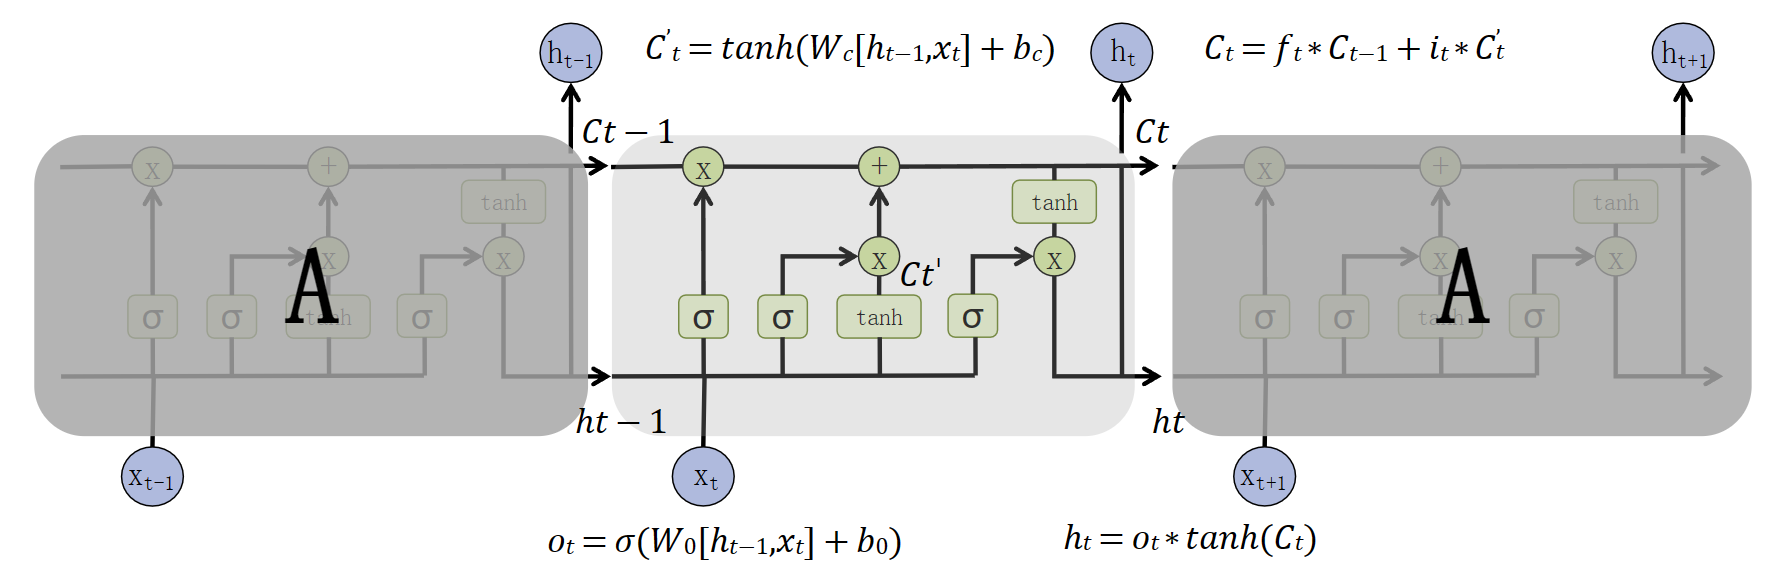
\includegraphics[width=0.9\linewidth]{figures/30.png}
    \caption{LSTM原理图}
    \label{fig:enter-label}
\end{figure}

假设在时间步 t,LSTM接收到输入向量 $x_t$ 和上一个时间步的输出 $h_{t-1}$以及细胞状态 $c_{t-1}$。

1. 
遗忘门:
\begin{equation}
f_t = \sigma(W_f \cdot [h_{t-1}, x_t] + b_f)
\end{equation}

$f_t$ 是遗忘门的输出,$W_f$ 是遗忘门的权重矩阵,$b_f$ 是偏置项,$\sigma$ 是$sigmoid$函数,它确保输出值在0和1之间,决定了要从细胞状态中遗忘多少信息。

2. 
输入门和候选细胞状态:
\begin{equation}
i_t = \sigma(W_i \cdot [h_{t-1}, x_t] + b_i)
\\
\tilde{c}_t = \tanh(W_c \cdot [h_{t-1}, x_t] + b_c)
\end{equation}

输入门决定了我们将在细胞状态中更新多少新信息,而候选细胞状态则提供了一个新的候选信息集,这些信息可能会被添加到细胞状态中。

3. 
细胞状态更新:
\begin{equation}
c_t = f_t * c_{t-1} + i_t * \tilde{c}_t
\end{equation}


当前细胞状态$c_t$是前一状态$c_{t-1}$经过遗忘门“遗忘”一部分后,与新的候选细胞状态经过输入门“筛选”一部分后相加得到的。

4. 
输出门和输出值: 
\begin{equation}
o_t = \sigma(W_o \cdot [h_{t-1}, x_t] + b_o)
\\
h_t = o_t * \tanh(c_t)
\end{equation}

输出门决定了哪些细胞状态的信息将输出,而输出值$h_t$则是这部分信息经过处理后用于传递到下一个LSTM单元或用于当前单元的输出。

这些公式共同定义了LSTM单元如何通过时间传递和更新信息,使其能够捕捉长期依赖关系。在本篇报告中,在预测数字农业渗透率、城乡就业人员、城乡总人口时采用了LSTM对接下来几年进行了时间预测。

\section{DLF}
双逻辑函数(Double Logistic Function, DLF)是一种适用于受到多重因素影响,既有增长又有减少的进行动态复杂变化的数学模型,比如人口。双逻辑函数通过结合两个逻辑函数,更加灵活地模拟出人口先增长后减少或反之的变化情况,如下图所示:
\begin{figure}[h]
    \centering
    \begin{minipage}[b]{0.45\textwidth}
        \centering
        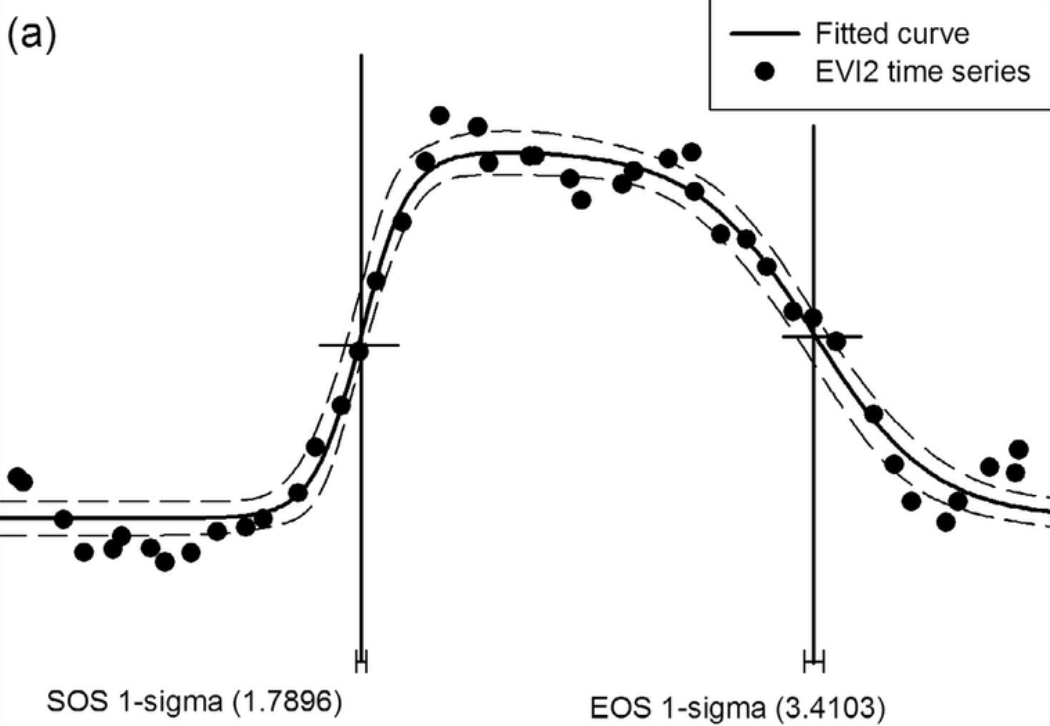
\includegraphics[width=\linewidth]{figures/53.png}
  
        \label{fig:first-image}
    \end{minipage}
    \hspace{0.05\textwidth} % Optional, add space between the images
    \begin{minipage}[b]{0.45\textwidth}
        \centering
        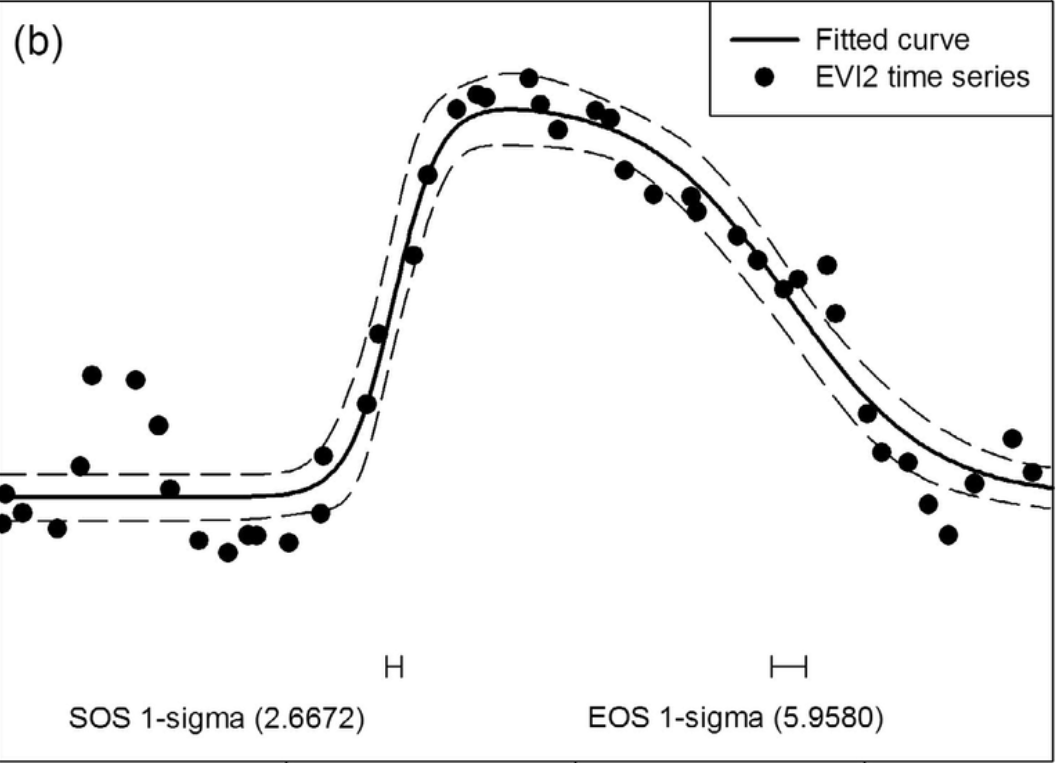
\includegraphics[width=\linewidth]{figures/54.png}
        
        \label{fig:second-image}
    \end{minipage}
    \caption{双逻辑函数进行曲线拟合}
\end{figure}

双逻辑函数的模型公式为:

\begin{equation}
P(t) = \frac{K}{1 + e^{-r(t - t_0)}} + \frac{L}{1 + e^{-s(t - t_1)}}
\end{equation}

其中$K$和$L$表示增长和减少的幅度,$r$和$s$是相应的增长率,$t_0$和$t_1$是拐点时间。

相比单一逻辑函数,双逻辑函数具有灵活性强、精度高和直观性好的优势。假设一个城市在某段时间内经历了快速人口增长,随后由于某些原因(如经济衰退、自然灾害)导致人口减少。利用双逻辑函数,可以分别设定增长和减少的幅度、速度和时间点,精确模拟出这一变化过程,提供有效的预测和分析工具。

\section{DLF-LSTM}
由于我们所获得的数据大部分与年份相关,且数据量较少,容易产生过拟合的情况。单纯依赖数学模型难以准确捕捉数据中的依赖关系,也无法拟合随着外部因素动态变化的信息。因此,我们考虑将两种模型进行融合,结合数学模型的精确性和机器学习模型的适应性,以提高整体模型的表现。

在本文中,我们选择双逻辑函数(DLF)和长短期记忆网络(LSTM)作为基学习器,同时处理相同的训练集,将得到的参数放入同一个数据集,并作为输入值输入到元学习器中。

\begin{figure}[H]
    \centering
    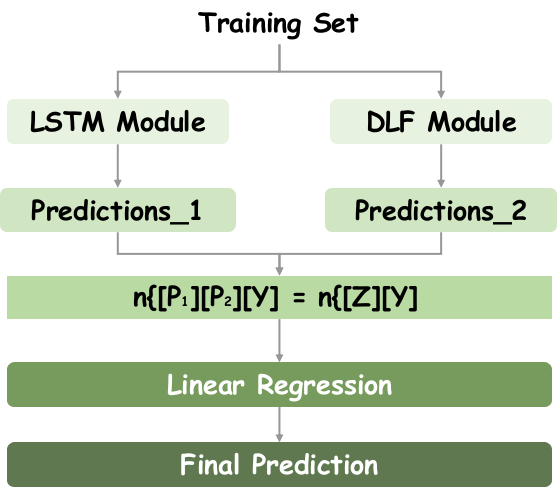
\includegraphics[width=0.45\linewidth]{figures/51.png}
    \caption{DLF-LSTM模型架构图}
    \label{fig:enter-label}
\end{figure}

尽管线性回归在处理非线性数据时可能存在一定的局限性,因为它本质上是线性的,但由于我们已经使用了双逻辑函数和LSTM对数据进行了非线性处理,线性回归可以有效地作为元学习器来整合这些非线性模型的输出结果。
\begin{algorithm}[H] % This keeps the algorithm where it is in the text
\caption{DLF-LSTM}
\begin{algorithmic}[1]
\State Initialize models: Double Logistic Function (DLF) and LSTM
\State Prepare dataset $D$, split into $D_{\text{train}}$ and $D_{\text{test}}$
\State \textbf{Train DLF and LSTM:}
\For{$(x_i, y_i) \in D_{\text{train}}$}
    \State Predict $y_{\text{DLF}}^i \leftarrow \text{DLF}(x_i)$ and $y_{\text{LSTM}}^i \leftarrow \text{LSTM}(x_i)$
    \State Store predictions
\EndFor
\State Combine predictions into new feature set $X_{\text{meta}}$
\State \textbf{Train Linear Regression Meta-Learner:}
\State Train on $X_{\text{meta}}$ to predict $y_i$
\State \textbf{Evaluate Model on $D_{\text{test}}$:}
\For{$(x_i, y_i) \in D_{\text{test}}$}
    \State Predict $y_{\text{pred}}^i$ and compute accuracy
\EndFor
\State Output the overall performance
\end{algorithmic}
\end{algorithm}
使用“堆叠回归”(Stacked Regression)的方法将DLF和LSTM融合,能够在一定程度上实现两者的互补,充分发挥各自的优势,从而提高整体模型的预测准确性和鲁棒性。

\section{模型对比}
我们对融合之后的 DLF-LSTM 模型与其他模型及融合之前的模型进行了对比,比较了不同机器学习模型在测试集上的性能,尤其是在误差(MSE、RMSE)和模型解释能力(R²)方面,结果如下图所示。

\begin{figure}[H]
    \centering
    \begin{subfigure}[b]{0.6\linewidth}
        \centering
        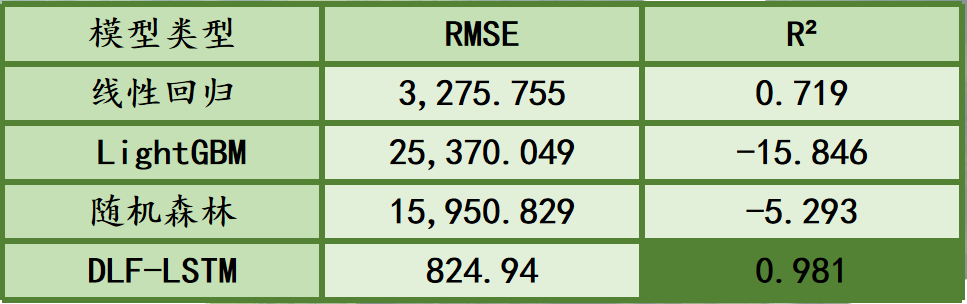
\includegraphics[width=\linewidth]{figures/55.png}
     
        \label{fig:enter-label-1}
    \end{subfigure}%
    \\
    \begin{subfigure}[b]{0.6\linewidth}
        \centering
        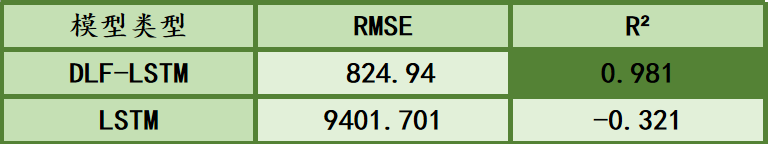
\includegraphics[width=\linewidth]{figures/56.png}
        
        \label{fig:enter-label-2}
    \end{subfigure}
    \caption{与原先模型的对比}
    \label{fig:combined-label}
\end{figure}

从图表中可以看出,DLF-LSTM 模型在所有指标上表现最优,具有最低的 MSE 和 RMSE,以及非常高的 R² 值,显示了出色的预测能力和数据拟合度。相比之下,其他模型的表现则不尽如人意。例如,随机森林模型出现了过拟合现象;LightGBM 的 R² 值甚至为负,显示其在测试集上的表现非常差;线性回归模型的准确率不高,难以胜任复杂的预测任务。

对比融合之前的模型,LSTM 的 RMSE 明显高于 DLF-LSTM,表明其在测试集上的预测误差较大。此外,LSTM 的 R² 值为负,表示其在测试集上的表现甚至比基于数据平均值的简单模型还要差,这是典型的过拟合迹象。

总体而言,DLF-LSTM 模型展示了非常低的误差和高度的数据拟合能力(R² 接近 1),表明其具有优越的性能,能够有效地避免过拟合,并在未见数据上提供可靠的预测。而标准 LSTM 模型则可能需要进一步的参数调整和正则化以改善其泛化能力。

这个对比结果表明,DLF-LSTM 模型在各种指标上均表现出色,是一个更为优越的特定于少量时序数据的选择,能够在复杂的预测任务中提供更高的准确性和可靠性。

\chapter{背景}
\label{chapter:introduction}
\section{两会中的乡村发展}
在中国这片辽阔的土地上,城市的霓虹灯光下掩映着农村的静谧星空。改革开放以来,中国经历了翻天覆地的变化。城市化与工业化的巨轮迅速推进,城乡人口结构发生巨大改变,同时也带来一系列“三农”问题。在这样的背景下,乡村振兴战略的提出成为解决社会主要矛盾的必然需求,是推动城乡协调发展的关键举措。

党的十四届全国人大二次会议中多次提到,推进乡村全面振兴是新时代新征程“三农”工作的总抓手,要锚定建设农业强国目标,学习运用“千万工程”经验,以加快农业农村现代化更好推进中国式现代化建设。要坚持农业农村优先发展,加快现代农业建设,全方位夯实粮食安全根基,多途径促进农民收入较快增长。要坚持农民主体地位,大力培养乡村人才,吸引各类人才投身乡村振兴。要深入推进农村生态文明建设,加快发展方式绿色转型,建设宜居宜业和美乡村。

本文通过爬虫技术梳理了全国两会报告中涉及乡村发展的所有内容,旨在彰显国家对乡村振兴战略的高度重视。
\begin{figure}[H]
    \centering
    \begin{minipage}{0.5\textwidth}
        \centering
        
\includegraphics[width=\linewidth]{figures/33.png}
        
        \label{fig:enter-label}
    \end{minipage}\hfill
    \begin{minipage}{0.5\textwidth}
        \centering
        
\includegraphics[width=\linewidth]{figures/6.png}
        
        \label{fig:TwoSessions}
    \end{minipage}
    \caption{两会爬虫文本看乡村发展必要性}
\end{figure}

自党的十九大报告首次提出实施乡村振兴战略以来,中国在“三农”工作上已取得了一定成就,本文收集并整理了近年来的相关数据,致力于分析农村发展历程。

\section{角度分析}

在了解到国家高度重视乡村振兴战略的基础上,本文将站在乡村发展的视角上深入探讨这一战略。通过整合《全国乡村产业发展规划(2020-2025年)》的相关文本并筛选出关键词汇,以词云的形式展现本文分析乡村发展的核心内容。

\begin{figure}[H]
    \centering
    
\includegraphics[width=0.6\linewidth]{figures/46.png}
    \caption{全国乡村产业发展规划词云图}
    \label{fig:enter-label}
\end{figure}

在词云中突显出诸多关键词,如“农产品”、“休闲”、“创新创业”、“建设”、“旅游”、“农民”和“就业”等,体现出乡村振兴战略的多维焦点,也为本文后续的论述指明方向。因此,本文将以这些关键词作为基础,解析它们在乡村振兴过程中的具体含义与作用,进而深化对该战略全局性和战术性贯彻落实的认识。
\chapter{粮食安全问题}
\label{chapter:Food security problem}

习近平总书记指出,粮食安全是“国之大者”,耕地是粮食生产的命根子,确保18亿亩耕地红线决不突破。

在全球化的背景下,粮食安全问题成为国际社会关注的焦点。作为世界上人口数量位居前列的国家,中国在粮食安全方面的表现不仅关乎其经济发展和社会稳定,还对维护全球粮食安全体系发挥着关键作用。而农村地区,作为粮食生产的主要基地,承担着维护国家粮食安全的重要责任。

\section{农作物播种面积}

粮食安全的基础在很大程度上依赖于稳定且充足的播种面积。播种面积不仅直接影响到粮食的总产量,也关系到农业的可持续性和对环境变化的适应能力。本文收集到了1990-2022年的农作物总播种面积。为直观分析这一时期内播种面积的波动和趋势,本文计算出播种面积的平均值,并利用玫瑰图展示各年度播种面积相对于平均值的变化,如下图所示:
\begin{figure}[H]
    \centering
    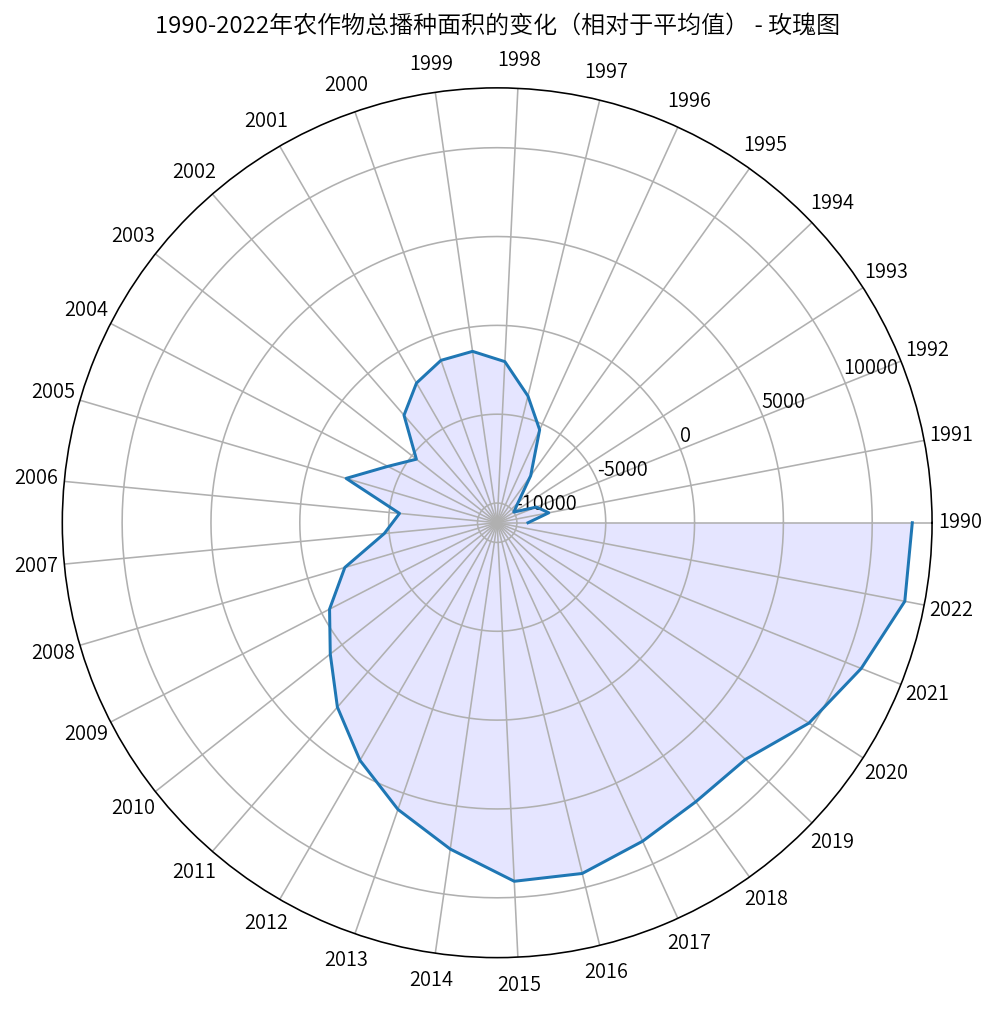
\includegraphics[width=0.5\linewidth]{figures/5.png}
    \caption{1990-2022年农作物总播种面积变化图}
    \label{fig:Total_sown_area}
\end{figure}

从图中可以看出,大多数花瓣沿着径向向外扩展,这表明随着时间的推进,播种面积呈现出增长趋势。这种增长通常指示了农业用地的扩张,对粮食安全来说是一个积极的信号,因为这意味着有潜力生产更多的粮食来满足日益增长的人口需求。同时,这样的增长也应当与生态和可持续发展原则相协调。

\section{主要粮食产量}

通过阅读农业农村部门文件农办科〔2023〕15号以及其他相关文献,可以了解到中国的农业生产主要集中在小麦、稻谷、大豆和玉米等主食农作物上。这些作物的生产状况对我国的粮食安全至关重要。

同样,本文收集了1990年到2022年间的粮食产量数据。为了更清晰地展示近年来的发展趋势,本文截取了2005年至2022年间的数据绘制了折线图,如下图所示:

\begin{figure}[H]
    \centering    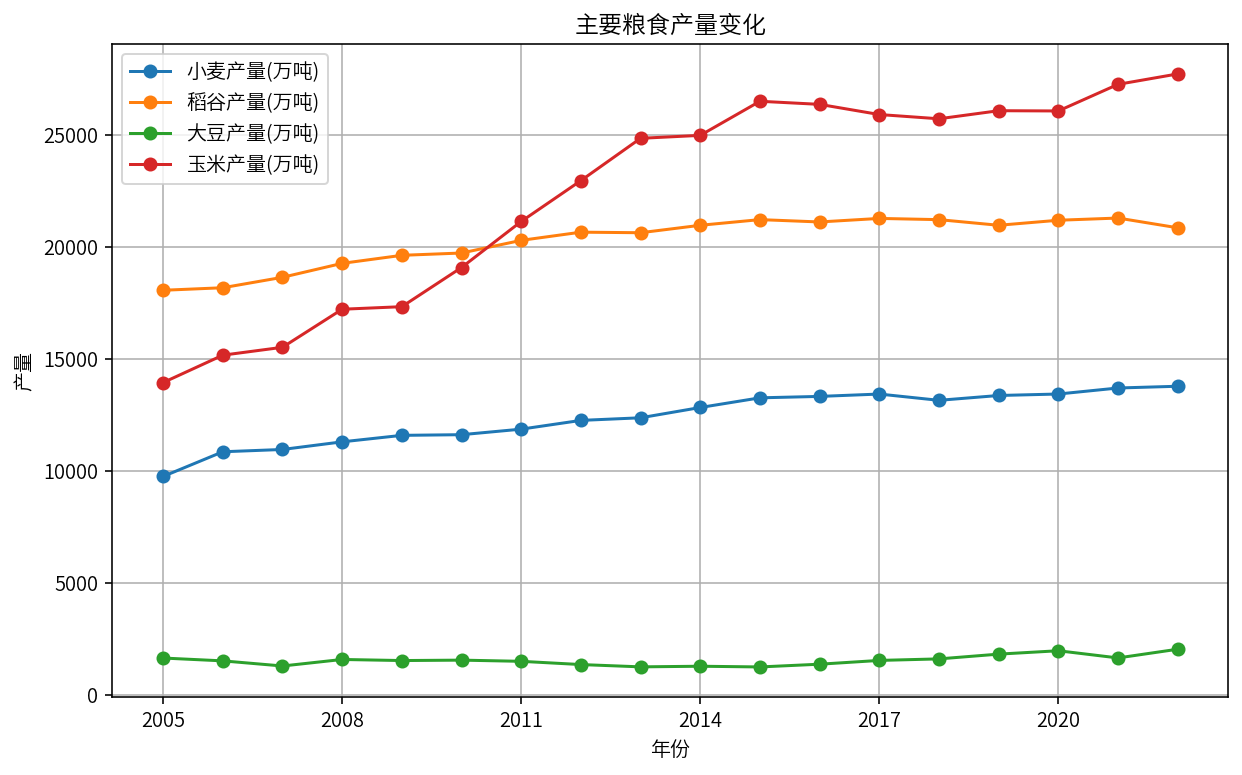
\includegraphics[width=0.9 \linewidth]{figures/8.png}
    \caption{主要粮食产量变化}   \label{fig:Changes_grain_production}
\end{figure}

此折线图清晰地呈现了自2005年以来中国主要粮食作物的产量变化。显著的是,水稻、小麦和玉米三者的产量逐年攀升,这一趋势不仅标志着农业技术进步和生产效率的提高,也反映了中国乡村振兴策略成功增强了农村地区的农业生产能力。鉴于这些作物在中国饮食中占据基础性地位,它们产量的增加直接增强了国家粮食安全保障。

此外,在十四届全国人民代表大会第二次会议上,国务院提出了我国粮食库存消费比的最新数据,显示我国的粮食库存消费比远高于联合国粮农组织建议的17\%-18\%的国际安全水平。这一数据不仅展示了我国在粮食安全领域所取得的显著成就,也反映了国家对于保障粮食安全的高度重视和扎实努力。
\chapter{科技进步}
\label{chapter:technology}
《“十四五”推进农业农村现代化规划》提出\cite{national-agricultural-green-development-plan},计划到2025年,农业基础更加稳固,乡村振兴战略全面推进,农业农村现代化取得重要进展。科技的进步显著推动了乡村发展,不仅改变了农村的面貌,也为乡村振兴注入了新的活力\cite{农办科〔2023〕15号附件}。
以下是十四五规划的规划目标图:
\begin{figure}[h]
    \centering
    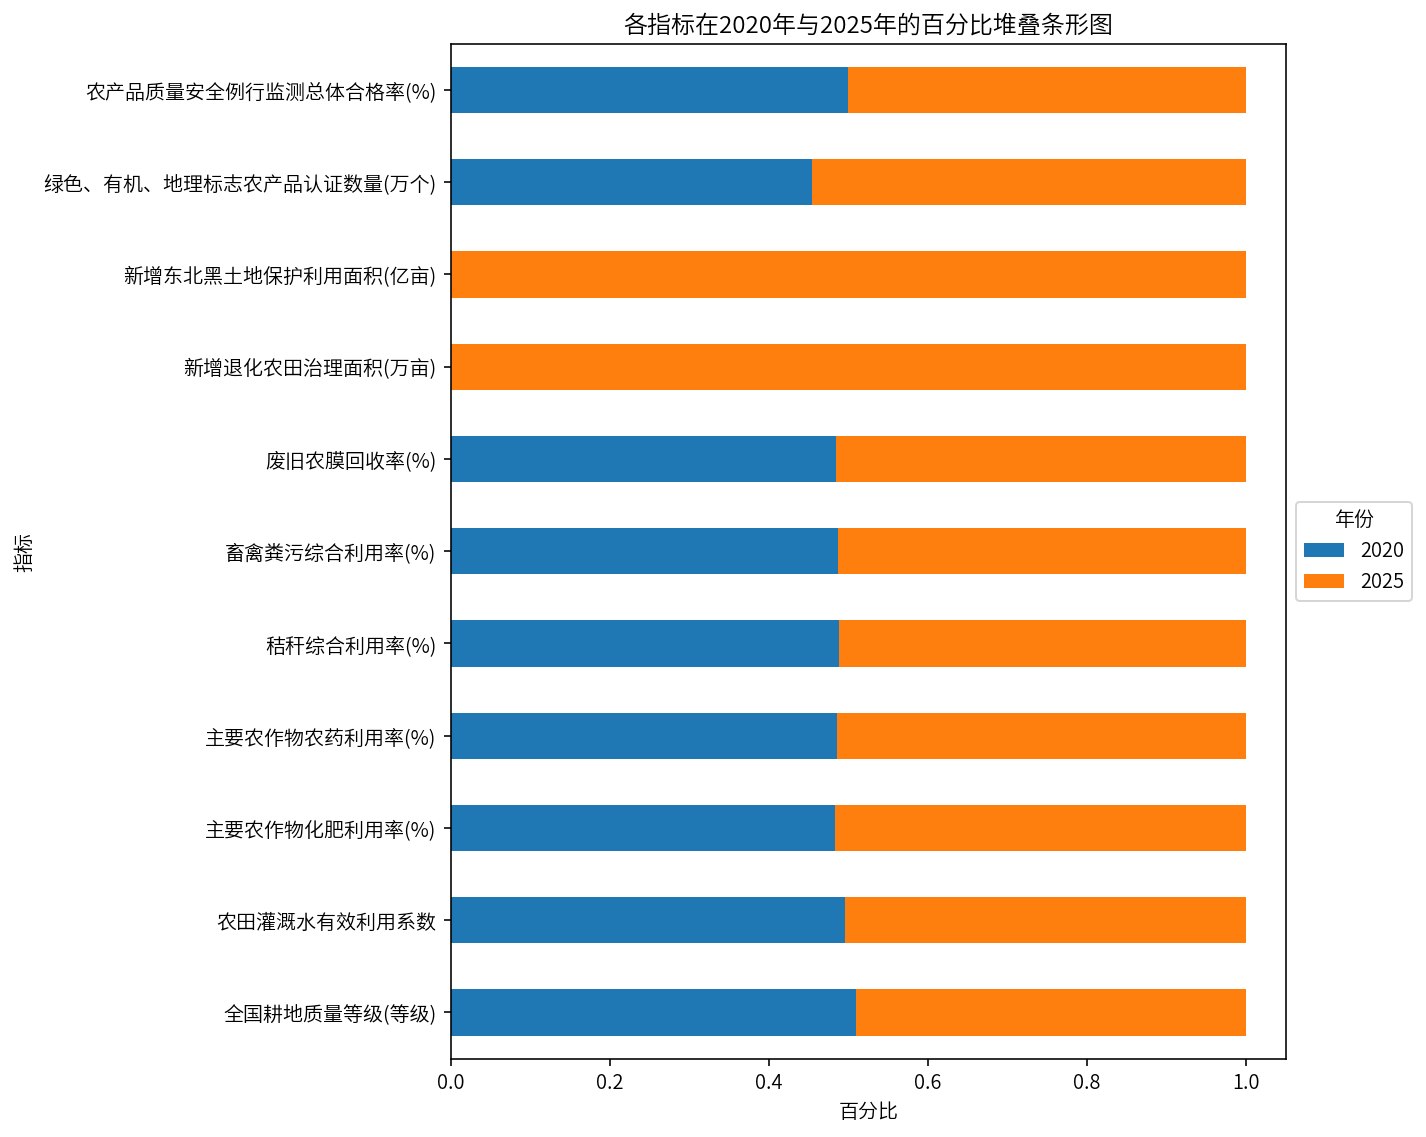
\includegraphics[width=0.7\linewidth]{figures/41.png}
    \caption{十四五规划流程目标图}
    \label{fig:enter-label}
\end{figure}

\section{科技对乡村农业的发展的影响}
\subsection{科技主要贡献}
农业现代化是实现可持续发展的关键,而农业科技现代化则是推动农业现代化的核心。本文综合收集并分析了农业科技在全国范围内的核心指标,涵盖农业科技进步贡献率、化肥与农药的有效利用率,以及县域数字农业发展的现状。依据这些关键指标,搜集了相应的数据,并据此绘制了热力图,如下图所示:

\begin{figure}[H]
    \centering
    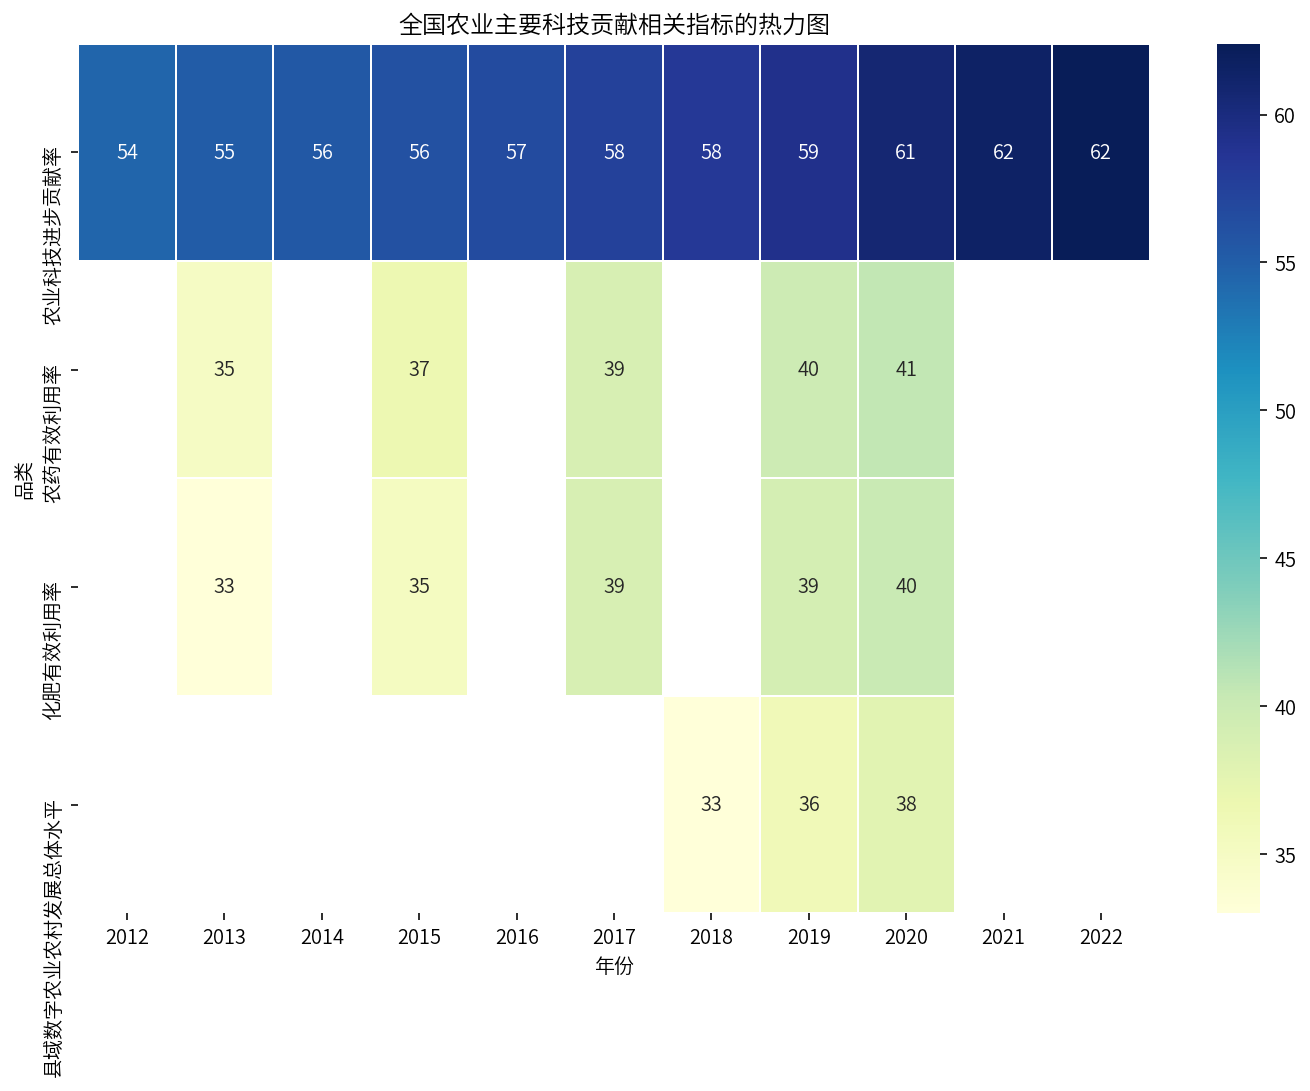
\includegraphics[width=0.5\linewidth]{figures/12.png}
    \caption{全国农业主要科技贡献相关指标的热力图}  
    \label{fig:Technology_hot}
\end{figure}

由图可知,科技在农业中的贡献逐年上升,体现在农业科技进步贡献率的持续增长。这不仅意味着科技创新在提高农业生产力方面起到了关键作用,而且反映出乡村经济正逐渐向技术密集型发展模式转变。

化肥和农药的有效利用率的增加,指向了农业生产过程中资源利用效率的提高。县域数字农业农村发展总体水平的提升也标志着信息技术在乡村振兴中的日益重要性,表明数字化转型在助力农业现代化和乡村经济发展中发挥着增效作用。
\subsection{数字农业渗透率}
随后,本文特别关注了数字农业渗透率这一关键指标,以评估技术如何在实际农业生产中得到应用并推动乡村经济的发展,绘制出如下的条形图\cite{china-digital-inclusion-development-report-2022}:

\begin{figure}[H]
    \centering
    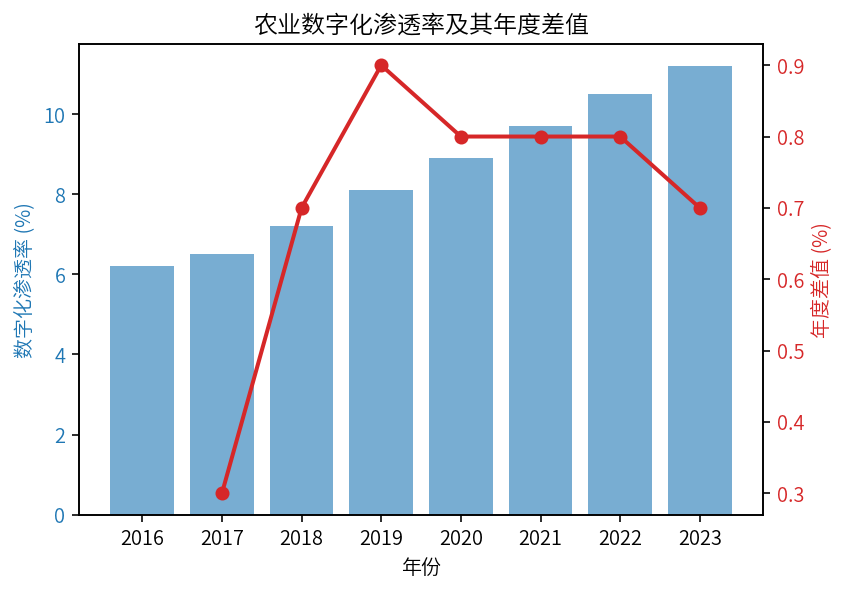
\includegraphics[width=0.6\linewidth]{figures/image1.png}
    \caption{数字农业渗透率折线图}
    \label{fig:Digital_agriculture_penetration}
\end{figure}

根据图表,可以看到农业数字化渗透率从2016年的0.062逐年增长,到2023年达到了0.112。从数字农业渗透率的变化趋势来看,数字化在农业中的应用呈现出逐年增长的态势,说明越来越多的农业生产活动正在通过数字技术进行优化和改进。

在本文中,采用了DLF-LSTM模型来对农业数字化渗透率进行建模和预测。在进行了详尽的测试之后,发现当学习率设置为0.004且经过100次迭代后,模型的损失率降至0.00138,并逐渐趋于稳定,这表明该模型达到了较高的预测精度。下面展示的图形描绘了模型训练过程中损失率的变化趋势,从中可以直观地观察到模型优化的效果和损失率随迭代次数的下降情况。

\begin{figure}[H]
    \centering
    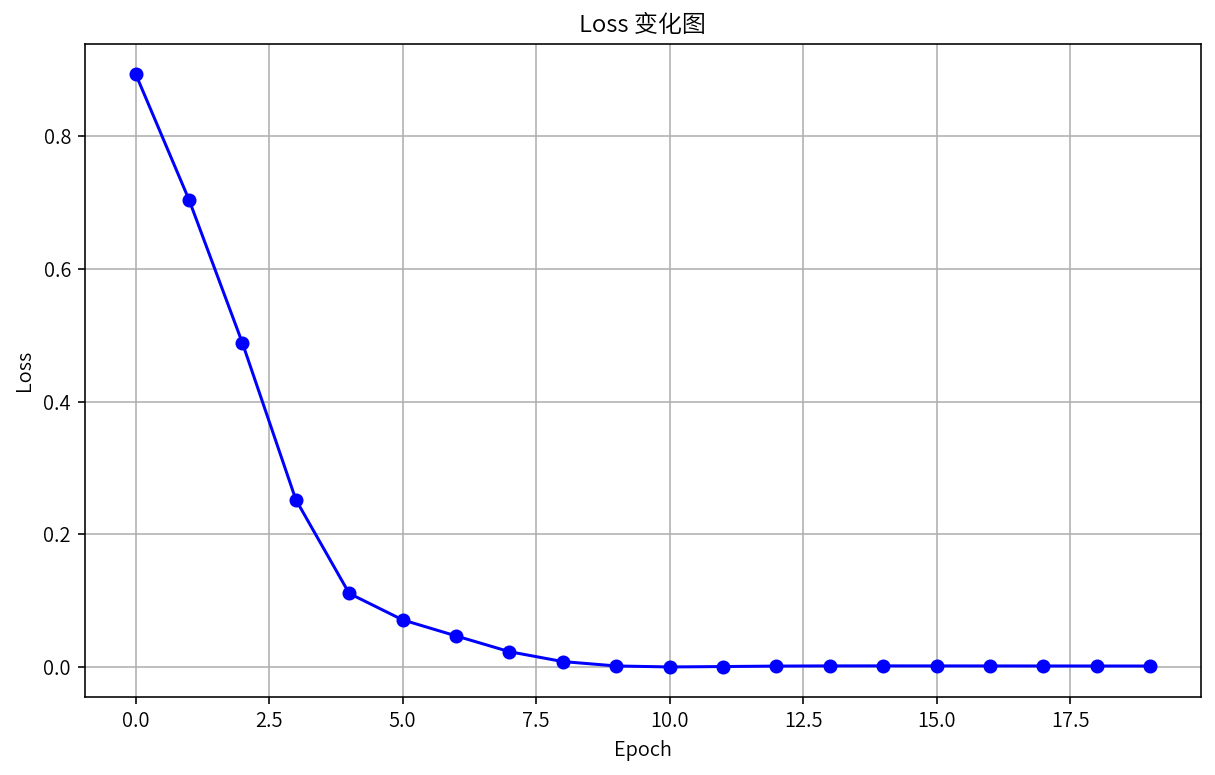
\includegraphics[width=0.65\linewidth]{figures/45.png}
    \caption{loss损失图}
    \label{fig:enter-label}
\end{figure}


预测数据如下表:
\begin{table}[H]
\caption{农业渗透话率预测表}
\centering
\begin{tabular}{cc}
\hline
\hline
\textbf{年份} &\textbf{预测农业渗透化率(万人)}\\
\hline
2024 & 0.12\\
2025 & 0.13\\
2026 & 0.14\\
2027 & 0.15\\
\hline
\end{tabular}
\end{table}

从预测数值来看,农业数字化渗透率在未来几年将保持稳步增长的态势。从2021年的0.12逐步增长到2027年的0.15,虽然整体呈现出向上的趋势,但增长幅度不是很大,且普及程度尚未达到预期的高水平。因此,可能需要进一步加大力度,推动数字技术在农业和乡村地区的广泛应用,以实现数字农业的全面渗透,带动乡村经济的全面发展。

\subsection{农业机械总动力}
在当前农业现代化的大背景下,农业机械化的推进尤显重要。本文借助国家统计局提供的权威数据,深入分析了我国农业机械化的发展态势。农业机械总动力,作为衡量农业机械化水平的重要指标,反映了全部农业机械动力的综合实力。绘制如下条形图进行分析:

\begin{figure}[H]
    \centering
    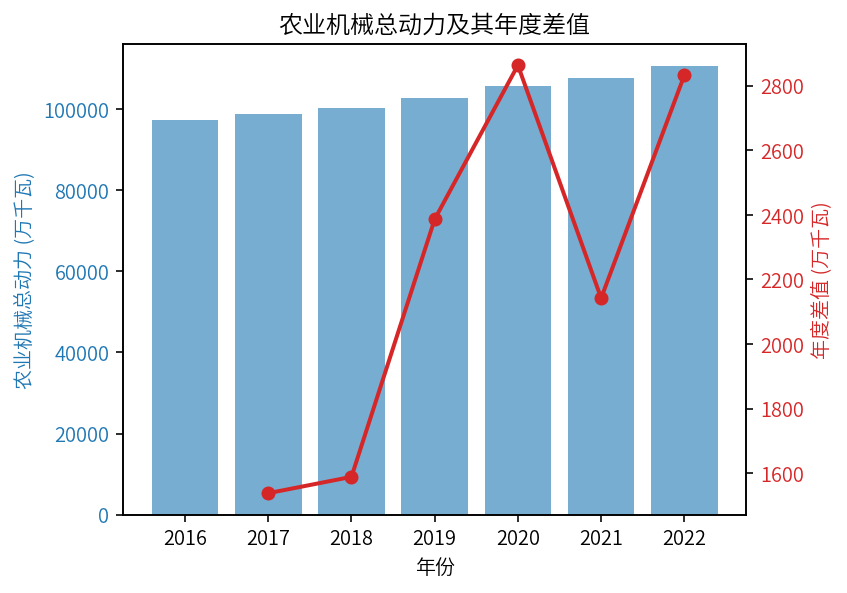
\includegraphics[width=0.6\linewidth]{figures/32.png}
    \caption{农业机械总动力条形图}
    \label{fig:agricultural_machinery_power}
\end{figure}

数据显示,我国农业机械总动力呈持续上升趋势。截至2022年,该指标达到了110597.19万千瓦,较去年增长了2800多万千瓦,展现了我国农业机械化快速发展的势头。

利用时间序列预测模型,进一步预测了未来的发展趋势。模型显示,若当前发展势头保持不变,农业机械总动力有望在未来几年内达到114378.54万千瓦。农业机械总动力的逐年提升,不仅彰显了国家在农机装备产业转型升级方面的坚定决心,也体现了农业农村部在推进“十四五”全国农业机械化发展规划中的积极作用\cite{china-digital-rural-development-2022}。
\begin{table}[H]
\caption{农业机械化预测表}
\centering
\begin{tabular}{cc}
\hline
\hline
\textbf{年份} &\textbf{未来农业机械总动力(万千瓦)}\\
\hline
2023 & 114378.54\\
2024 & 117931.49\\
2025 & 121980.57\\
\hline
\end{tabular}
\end{table}
农业机械化的持续发展是国家现代化农业战略的重要组成部分。随着政府对农业机械化的持续投入和政策支持,有理由相信,我国农业机械化的未来将更加光明,为实现乡村振兴战略贡献更大的力量。

\section{科技对乡村居民生活的影响}

随着我国乡村振兴战略的深入实施,科技创新力量不断渗透到乡村生活的各个层面,显著改变了广大农村居民的日常生活习惯和经济社会发展面貌。近年来,国家积极推动互联网基础设施向农村延伸,加快缩小城乡数字鸿沟,这一举措成效显著。

\begin{figure}[H]
    \centering
    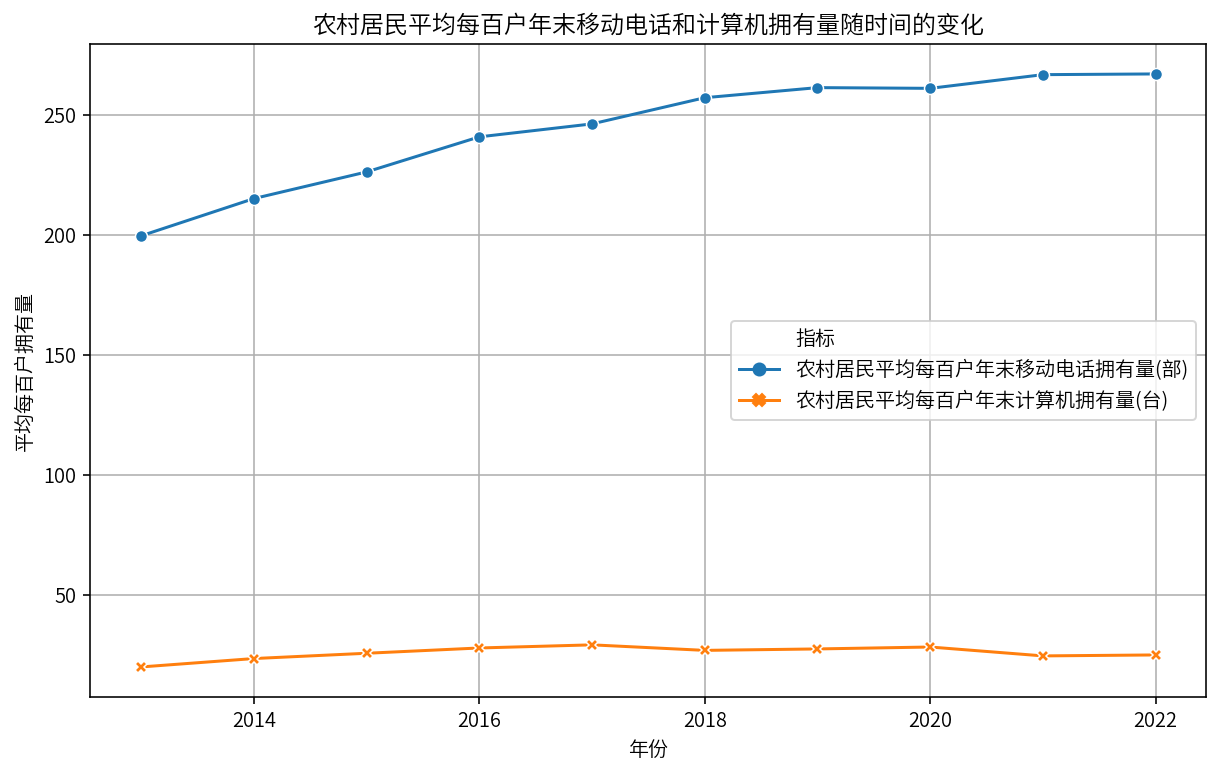
\includegraphics[width=0.65\linewidth]{figures/42.png}
    \caption{电子设备使用量序列图}
    \label{fig:enter-label}
\end{figure}

本文通过绘制时间序列的折线图,进而揭示了农村居民对电脑和手机这两类主要电子设备的使用趋势。随着互联网技术的广泛普及,可以观察到农村居民的手机拥有量呈现出显著的增长趋势,反映了移动设备在日常生活中的重要地位。相对而言,电脑的使用量在这段时间内变化不大,暗示着农村地区对于电脑的需求和应用场景仍然有限,或许是由于农村地区对高科技设备的适应性和接受度有待提高。

通过对城乡居民互联网使用状况的数据分析可以发现,无论是城市还是乡村,互联网普及率均呈现出稳步上升的趋势。特别是在过去几年间,随着移动互联网技术的普及和网络资费的下调,越来越多的农村居民得以接入互联网,享受到便捷高效的数字化服务\cite{digital-village-strategy}。

\begin{table}[H]
    \centering
    \caption{2020-2022城乡居民互联网使用量预测}
    \begin{tabular}{ccc}
        \hline
        \hline
        \textbf{年份} &\textbf{农村居民互联网使用量预测}&\textbf{城镇居民互联网使用量预测}\\
        \hline
        2020&63.680962&77.475733\\
        2022&82.730215&98.743864\\
        \hline
    \end{tabular}
    \label{tab:Internet}
\end{table}

本数据缺失2020到2022的数据,因此使用指数平滑法进行预测。结合趋势推测,当前城乡互联网用户的比例可能接近于5:4这样一个水平,预示着乡村互联网市场潜力巨大,并有望在未来进一步激活农村经济,助力乡村振兴战略目标的实现。

\begin{figure}[H]
    \centering
    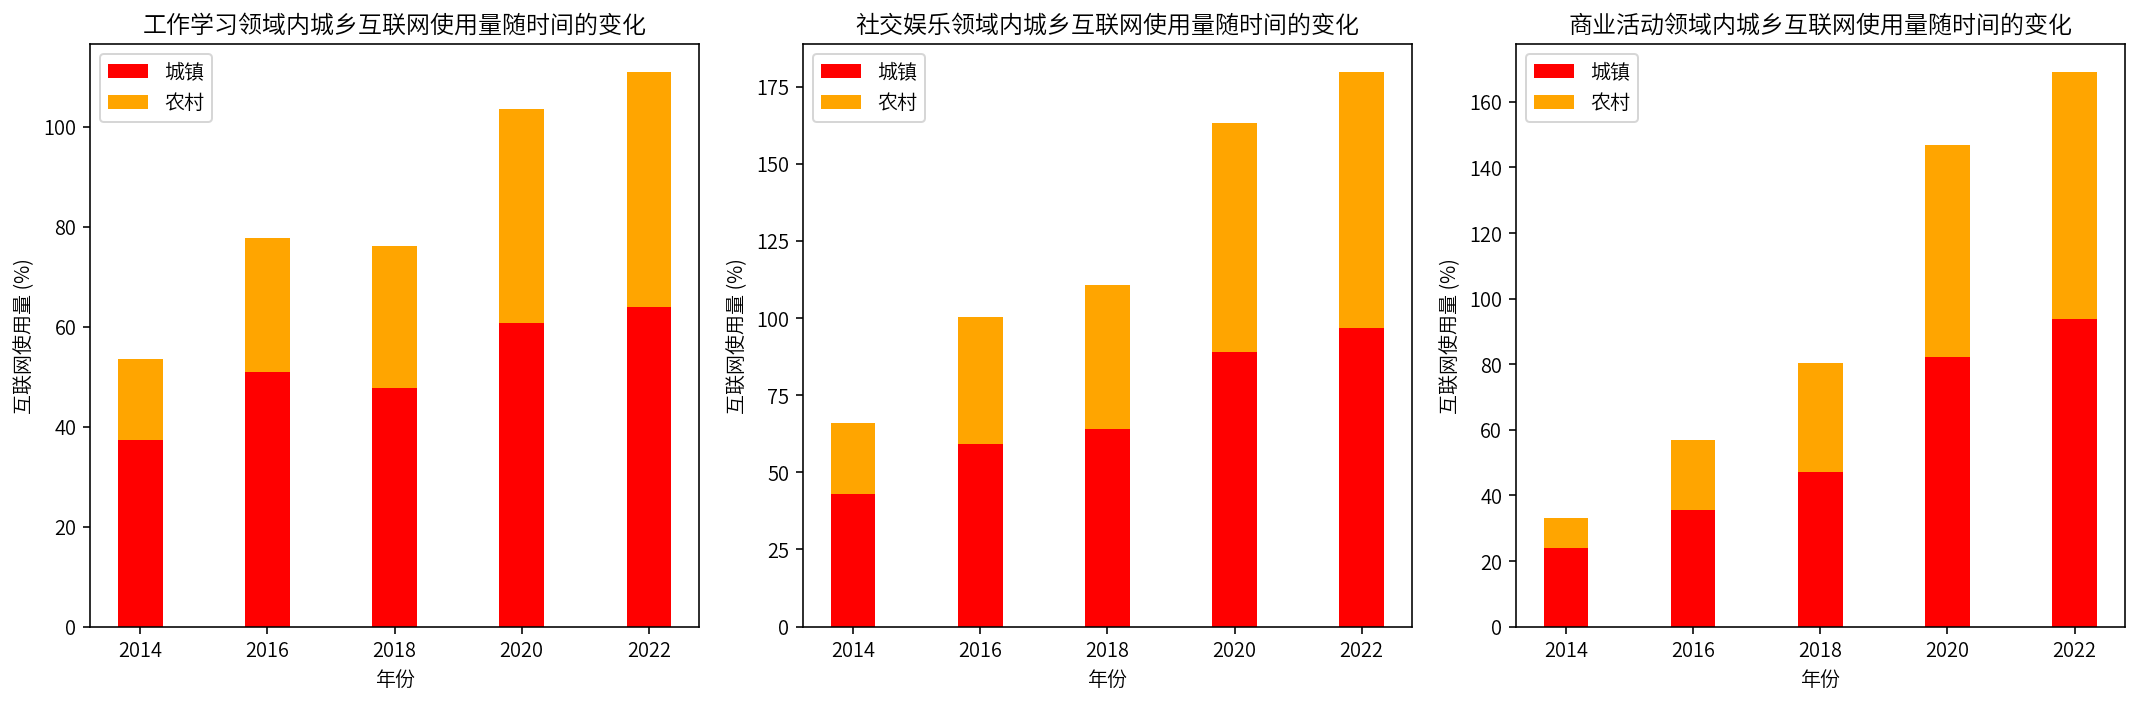
\includegraphics[width=1\linewidth]{figures/50.png}
    \caption{城乡互联网使用量随时间变化对比图}
    \label{fig:enter-label}
\end{figure}

数据显示,城乡间的互联网使用量差距正在逐年缩减。农村地区的互联网普及率不断提升,尤其是在商务交易、网络支付、信息获取等方面的应用率增长明显,这表明农村居民正加速融入数字经济的大潮之中。例如,农村网民通过电商平台进行农产品销售、利用网络平台开展技能培训、借助移动支付实现无现金交易等活动日益普遍。


这些数据共同映射了中国乡村经济在科技推动下的积极变化,揭示了科技进步是乡村振兴策略的关键驱动力。
\chapter{乡村建设}
\label{chapter:basic}

《乡村建设行动实施方案》指出:乡村建设是实施乡村振兴战略的重要任务,也是国家现代化建设的重要内容。

乡村基础设施的建设不仅是提升乡村生活品质的关键,更是吸引人才和促进人口回流的重要举措。此外乡村地区的文化和自然环境也是其独特的吸引力所在。

\section{基础设施建设}

在具体的基础设施建设中,为了量化评估进展和成效,本文选择了俩个关键性的指标:每万人拥有的卫生床数量和人均养老机构数量。这俩个指标不仅反映了乡村医疗卫生和养老服务设施的发展水平,也是衡量基础设施建设对提升居民生活质量影响的重要参数。

在收集近十年各地区的卫生床和人均养老机构数量数据的过程中\cite{heywhale-dataset},本文采用年复合增长率(CAGR)这一指标,将每个地区过去十年的数据统一转化,以便进行比较。同时进一步制作了一幅详尽的中国热力图,直观展现了各地区在所考察指标上的表现。

\begin{figure}[H]
    \centering
    \begin{minipage}{0.45\textwidth}
        \centering
        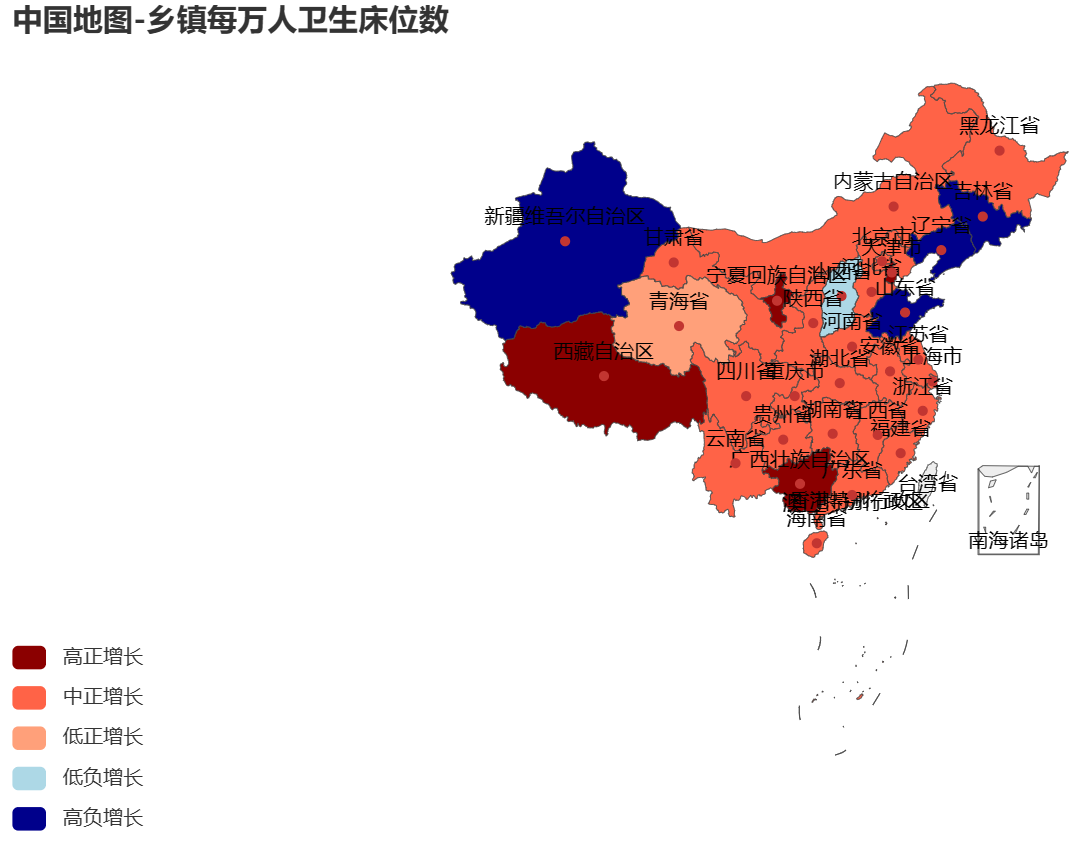
\includegraphics[width=\linewidth]{figures/18.png}
        \caption{卫生床位数}
        \label{fig:beds}
    \end{minipage}\hfill
    \begin{minipage}{0.45\textwidth}
        \centering
        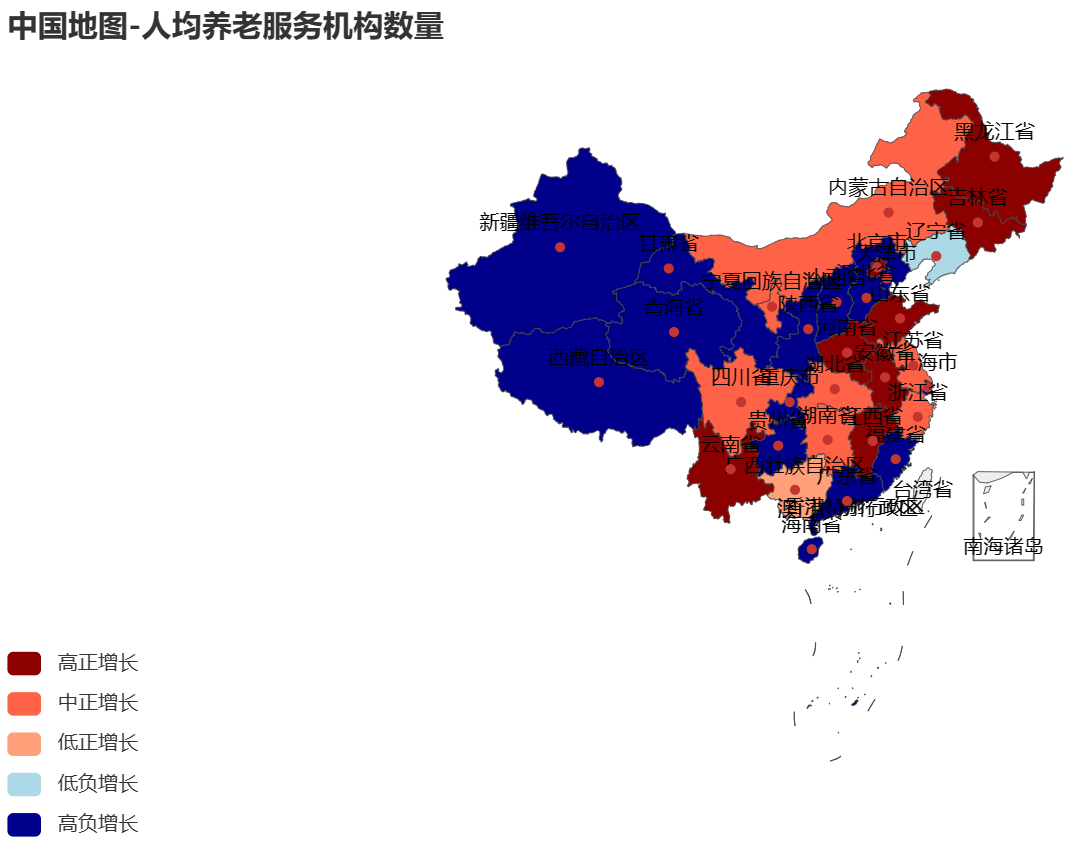
\includegraphics[width=\linewidth]{figures/17.png}
        \caption{养老机构数量}
        \label{fig:elderly-facilities}
    \end{minipage}
\end{figure}

在这两幅图中,红色区域表示正增长区域,蓝色区域表示负增长区域。颜色的深浅代表了增长的强度:红色越深表明正增长程度越高,蓝色越深则意味着负增长程度越显著。

结合胡焕庸线的地理分布来观察,在沿线东部地区,尤其是人口密集的乡镇,无论是卫生床位数还是养老机构数量,普遍呈现出正增长趋势。

然而,胡焕庸线以西的西部地区,尤其是人口较少的农村区域,却出现了卫生床位和养老机构数量的负增长趋势。这种情况在一些经济较发达的地区也有所体现,可能与这些地区的农村人口减少,需求降低有关。

这种差异性的现象揭示了我国农村在基础设施建设方面正处于一个积极变化的发展阶段。东部的积极增长反映了国家对农村地区尤其是人口密集区域的关注和投资的增加,显示出公共服务水平正在逐步提升,以适应居民不断增长的需求。而西部地区则突显了在人口减少的背景下,如何有效地规划和调整基础设施,以持续满足农村居民变化的需求。
\section{基础环境建设}

在推进乡村基础设施建设的过程中,必须同步加强对乡村自然环境的保护和改善,这对于实现乡村振兴和可持续发展具有至关重要的作用。

% "绿水青山就是金山银山"的发展理念深刻阐明了保护和改善自然环境不仅是对生态平衡的维护,更是推动经济和社会进步的关键路径。

本文对乡村环境进行了系统的量化分析,收集并研究了2015至2022年期间的关键环境指标数据\cite{rural-revitalization-environmental-report-2022}。这些数据包括村庄的供水情况、排水管道系统、人均绿地面积、环卫车辆的数量和使用情况以及公共厕所的配置和状况。通过计算连续两年之间的数据差值来确定每年的变化量,绘制出变化量与年份的关系图如下图所示\cite{农质发〔2023〕5号}:

\begin{figure}[H]
    \centering
    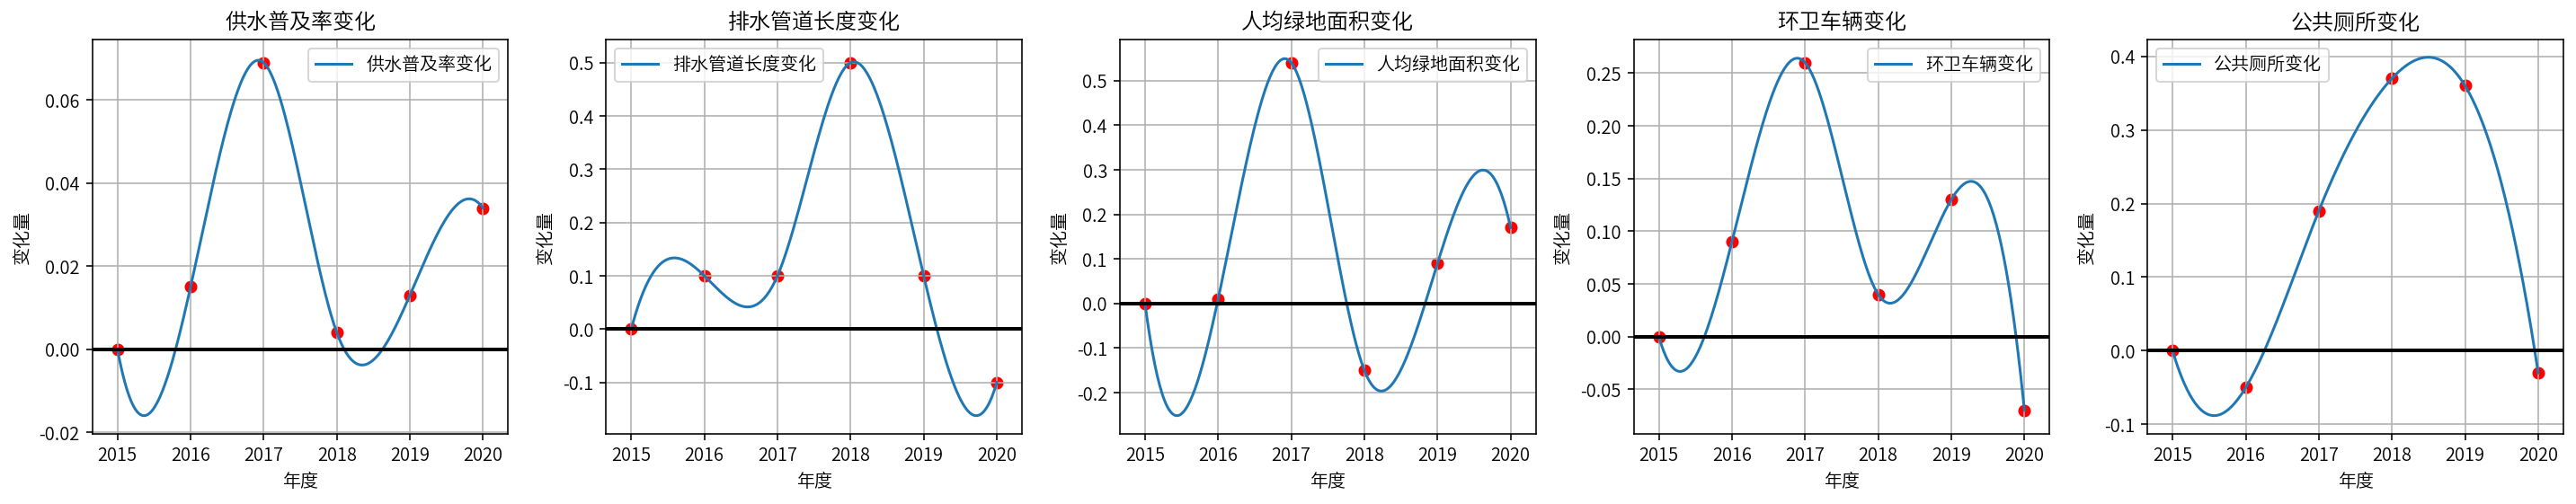
\includegraphics[width=1.0\linewidth]{figures/21.png}
    \caption{基础环境改善图}
    \label{fig:basic_environment}
\end{figure}

图表展示了多个指标随时间变化的趋势,其中大部分曲线持续处于零点线以上。这表明,尽管各指标呈现出明显的波动,总体上还是保持了增长态势。这一现象彰显了国家对基础设施与环境改善的坚定承诺。

\section{生态旅游建设}
乡村环境的改善已成为提升居民生活质量和健康水平的关键因素,同时也开辟了乡村经济转型升级的新路径。

环境质量的提升不仅吸引了生态旅游和绿色农业等绿色经济产业,也促成了新的经济增长点和增加了就业机会,为乡村带来了新的活力。本文深入分析了过去近十年来乡村旅游接待游客数量及其所带来的旅游总收入\cite{bisu-rural-tourism-report},绘制出如下图所示的柱状图:

% 在乡村振兴战略的推动下,乡村旅游特别成为了促进经济多样化、提高农民收入和加强城乡一体化的一个强有力的平台,展现了其在当前和未来乡村发展中的重要作用。

\begin{figure}[h]
    \centering
    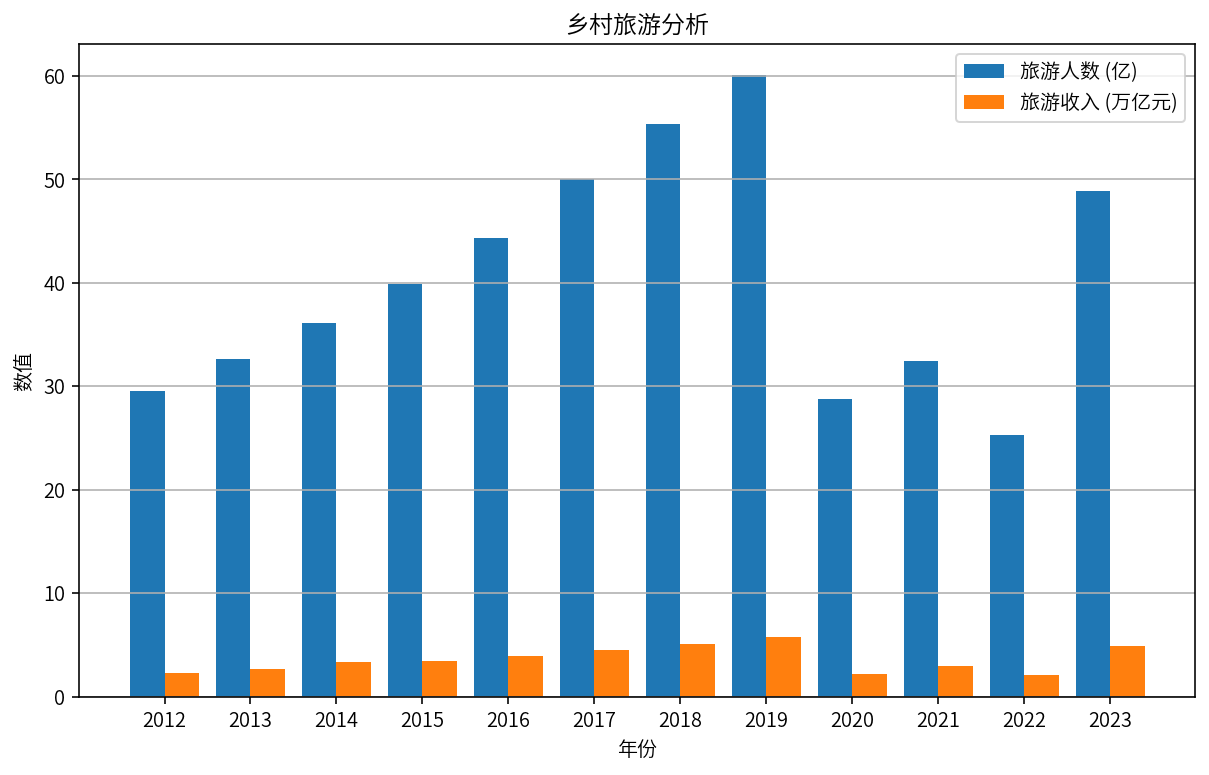
\includegraphics[width=0.65\linewidth]{figures/10.png}
    \caption{近十年乡村旅游人数与旅游收入}
\end{figure}

初期数据显示,乡村旅游人数和收入都呈现出稳步增长的态势,反映了人们对逃离城市喧嚣、探索自然和体验乡村生活愈发浓厚的兴趣。然而,2020年新冠疫情的爆发对我国旅游业造成了前所未有的打击,乡村旅游也未能幸免,其人次和收入均出现了急剧下滑。

随着疫情的结束,乡村旅游业开始呈现出复苏的势头,人们逐渐回归到了疫情前的生活和休闲模式。乡村旅游经历了一段迅猛的增长期,这种增长不仅归功于疫情的消退,乡村基础设施和环境设施的改善也在促进乡村旅游发展中发挥了至关重要的作用。

% 随着疫情逐步得到控制和政府的积极扶持,加之产业结构的优化和转型,乡村旅游开始展现出复苏的迹象。这一趋势不仅反映了乡村旅游的韧性和潜力,也预示着乡村旅游在后疫情时代将持续成为人们休闲和旅游的重要选择。

% 政府政策的支持和对乡村旅游潜力的认识促使相关产业链得到改善和升级,为乡村旅游的恢复提供了强有力的推动。经济逐步复苏,消费者信心增强,人们再次开始探索和享受乡村旅游带来的独特魅力,这促使乡村旅游的人次和收入逐渐恢复并呈现出积极的发展势头。
\chapter{ũ������ˮƽ}
\label{chapter:famer}
ũ����Ϊũ������壬������ũҵ������ֱ�Ӳ����ߣ�Ҳ��������ṹ�Ļ�������ˣ�ũ�������ˮƽ�Ǻ���ũ�徭�ú���ᷢչ����Ҫָ�꣬ũ�����������ĸ���ֱ��Ӱ�쵽ũ��Ŀɳ�����չ��
\section{ũ���ҵ}
\subsection{��ҵ�ṹ����}
���ž���ȫ�򻯵����뷢չ�������г��IJ������󣬿�ѧ����ȡ������������ũ������������������׷��������ǿ��ͬʱ��ũ�����֪ʶ���¼����Ľ��ܶ�Ҳ������ߣ�����֮��Ļ�������Ƶ�������롣��Щ���ع�ͬ���ã��ƶ���ũ���ҵ�ṹ�Ķ�Ԫ����չ��

\begin{figure}[h]
    \centering
    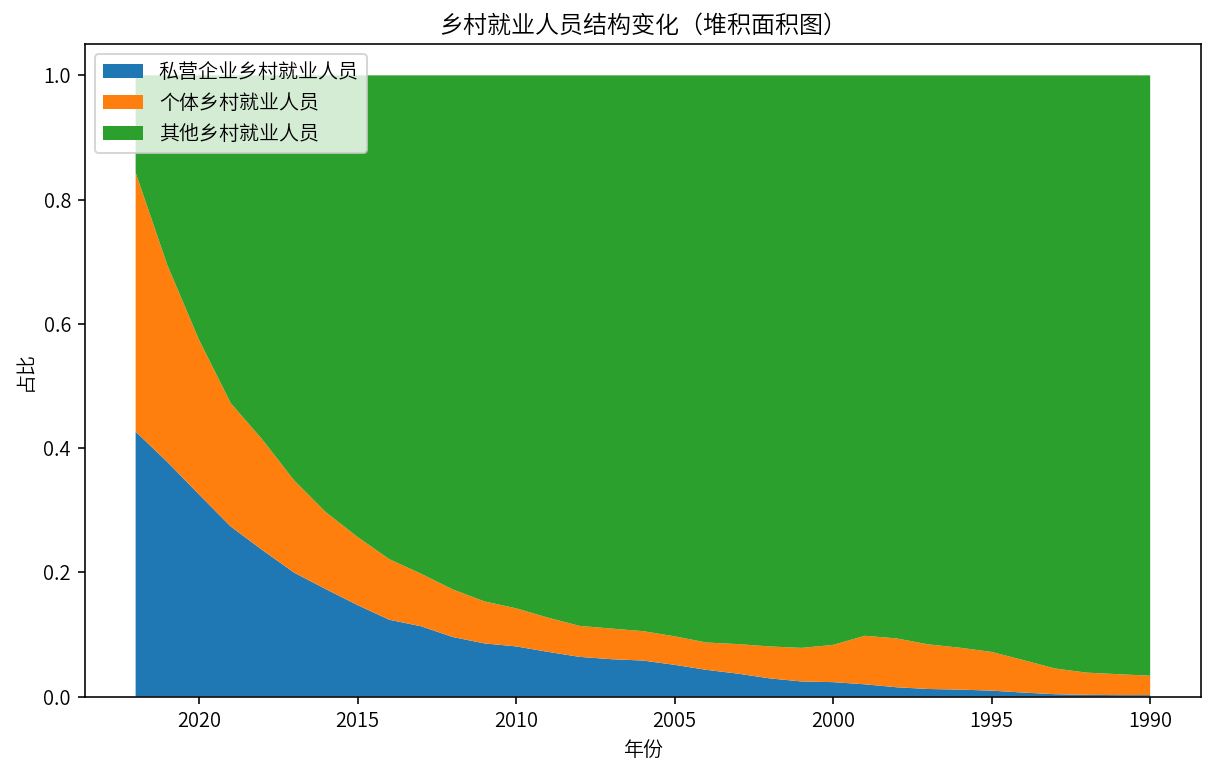
\includegraphics[width=0.75\linewidth]{figures/20.png}
    \caption{ũ���ҵ�ṹ�仯}
    \label{fig:struct_change}
\end{figure}

��ͼ�п��Թ۲쵽��˽Ӫ��ҵ�͸��廧�ھ�ҵ��Ա�еı������ֳ��������ƣ������ũ���ҵ�ṹ���ھ��������ı�����ڹ�ȥũҵ��������λ��ũ�徭�õĶ�Ԫ�������������ԡ���ũҵ��ӹ���������Ρ�ũ���ֵ����˲�ҵ�����������Ӿ�ҵ�����ͬʱ��Ҳ����طḻ��ũ��IJ�ҵ���ݡ�

\subsection{��ҵ��ԱԤ��}
�����ۺϷ�����1990����2022���ij����ҵ��Ա���ݣ���̽���ͳ��ֹ�ȥ��ʮ���г����ҵ�ṹ�ı�Ǩ���������ռ��Ĺ����У�����ijЩ��ݵ����ݴ���ȱʧ�����ΪNaNֵ�������ܻ�Ӱ��Ծ�ҵ���Ƶ�ȫ�������Ԥ�⡣Ϊ���ֲ���һ��ȱ��������������ԣ����ǿ��Dz���DLF-LSTMģ��������Ԥ�⡣

���ȣ�ģ��������״̬��Ԥ���˿�ȱ�����˽Ӫ��ҵ�ľ�ҵ������������ЩԤ����ֵת����ԭʼ��ģ������Ԥ��ͼ��������ͼ����ʾ����ʷ������ģ��Ԥ��ĶԱȡ�Ȼ��ʹ��ͬһģ�Ͷ�������ʷ���ݼ���������ϣ�ͬ���ؽ�Ԥ����ת����ԭʼ��ģ��ͨ�����ַ�ʽ�����˵ڶ���ͼ����չʾ��ģ�Ͷ���֪��ʷ���ݵ���ϳ̶ȡ�

\begin{figure}[h]
    \centering
    \begin{minipage}{0.45\linewidth}
        \centering
        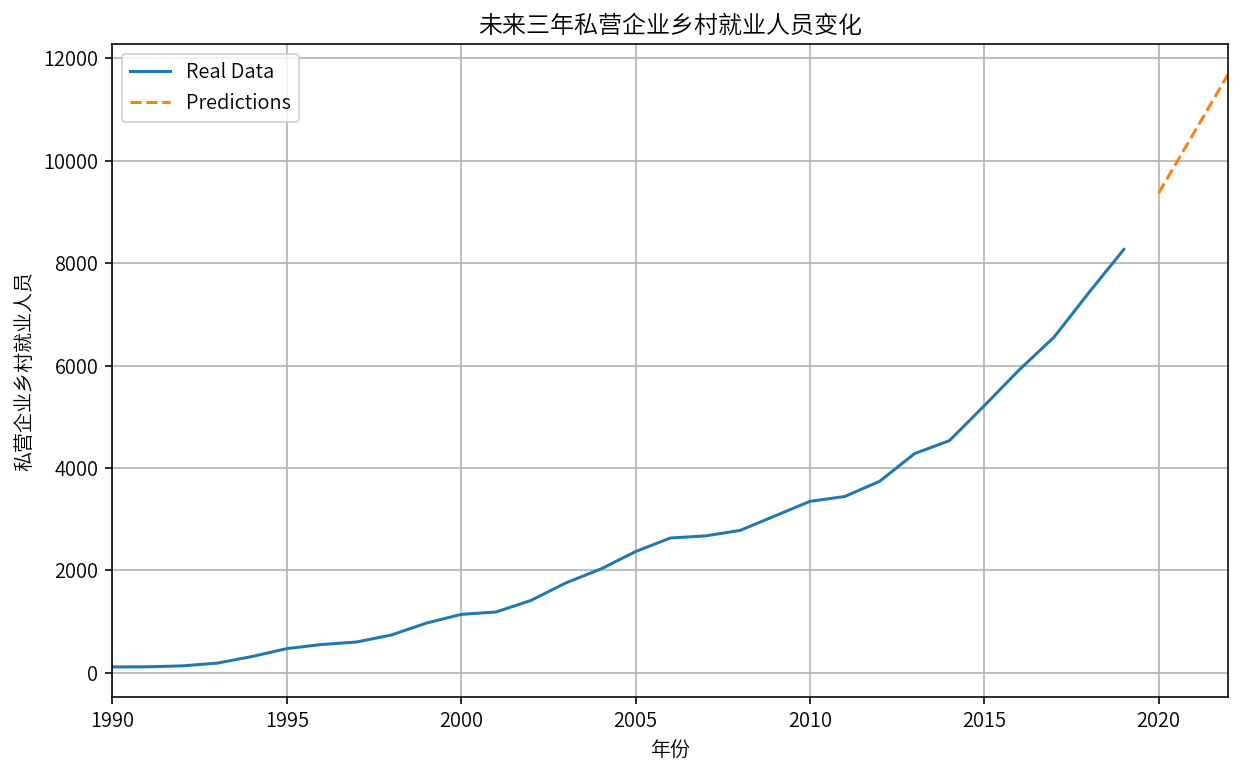
\includegraphics[width=\linewidth]{figures/22.png}
        \caption{δ������˽Ӫ��ҵ����ҵ��Ա�仯ͼ}
        \label{fig:prediction_private}
    \end{minipage}\hfill
    \begin{minipage}{0.45\linewidth}
        \centering
        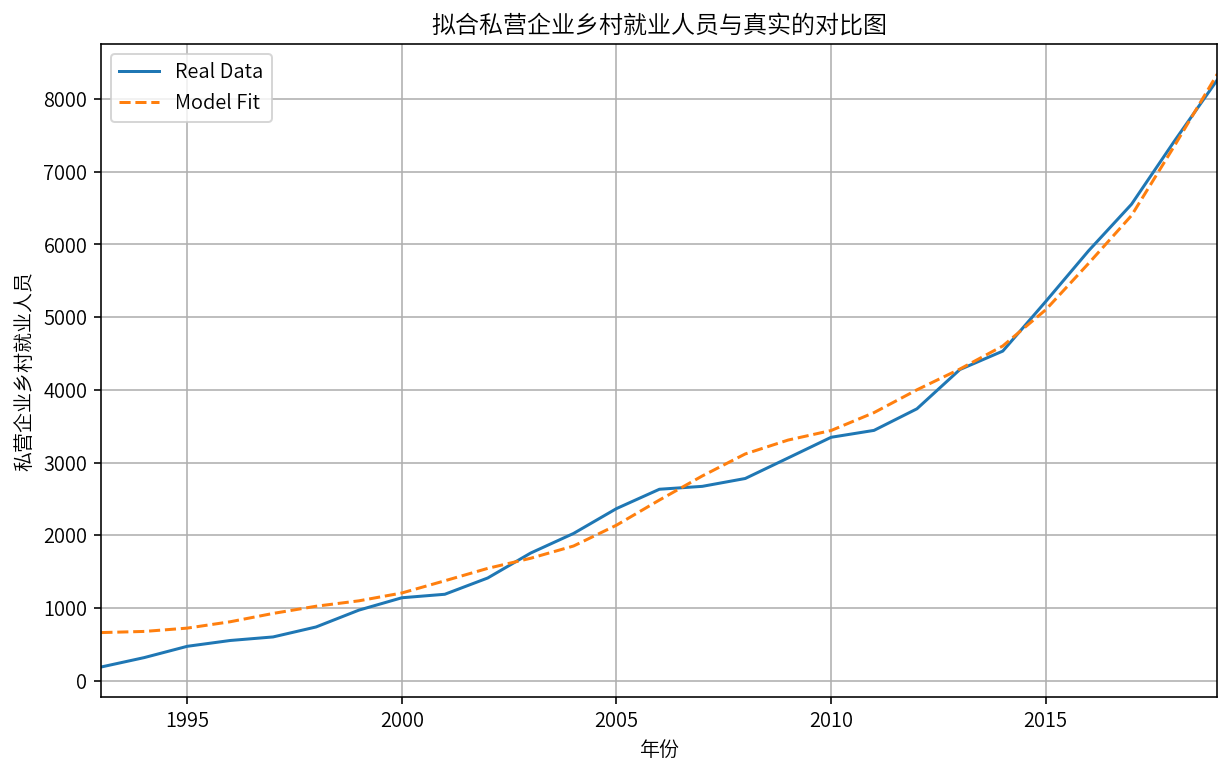
\includegraphics[width=\linewidth]{figures/23.png}
        \caption{���˽Ӫ��ҵ����ҵ��Ա����ʵ�ĶԱ�ͼ}
        \label{fig:fit-vs-real_private}
    \end{minipage}
\end{figure}

���������ֵ�ͼ�����������Թ۲쵽��ģ�;��нϸߵ���϶ȣ������ܹ���Ч��Ԥ�����ơ��������ģ�Ͷ���������˽Ӫ��ҵ��ҵ�����ı仯���пɿ��ԡ����ô�ģ�ͣ��ɹ�������������˽Ӫ��ҵ����ҵ��Ա�Ŀ�ȱ���ݲ�Ԥ���˺�����Ľ������ϸ������±���ʾ��


\begin{table}[H]
\caption{˽Ӫ��ҵ����ҵ��Ա����}
\begin{subtable}{0.5\textwidth}
  \centering
  \caption{��ȫ��ȱ����˽Ӫ��ҵ����ҵ��Ա}
  \begin{tabular}{cc}
    \hline
    \hline
    \textbf{���} & \textbf{˽Ӫ��ҵ����ҵ��Ա}\\
    \hline
    2020 & 9499.59\\
    2021 & 10732.58\\
    2022 & 12013.71\\
    \hline
  \end{tabular}
\end{subtable}%
\begin{subtable}{0.5\textwidth}
  \centering
  \caption{Ԥ������˽Ӫ��ҵ����ҵ��Ա}
  \begin{tabular}{cc}
    \hline
    \hline
    \textbf{���} & \textbf{˽Ӫ��ҵ����ҵ��Ա}\\
    \hline
    2023 & 13408.71\\
    2024 & 14651.86\\
    2025 & 15764.10\\
    \hline
  \end{tabular}
\end{subtable}

\end{table}


ͬ���أ�����Ҳ�Ը��廧����ҵ��Ա�����ݼ������˴���������������Ӧ��ͼ�������ݡ�

\begin{figure}[H]
    \centering
    \begin{minipage}{0.45\linewidth}
        \centering
        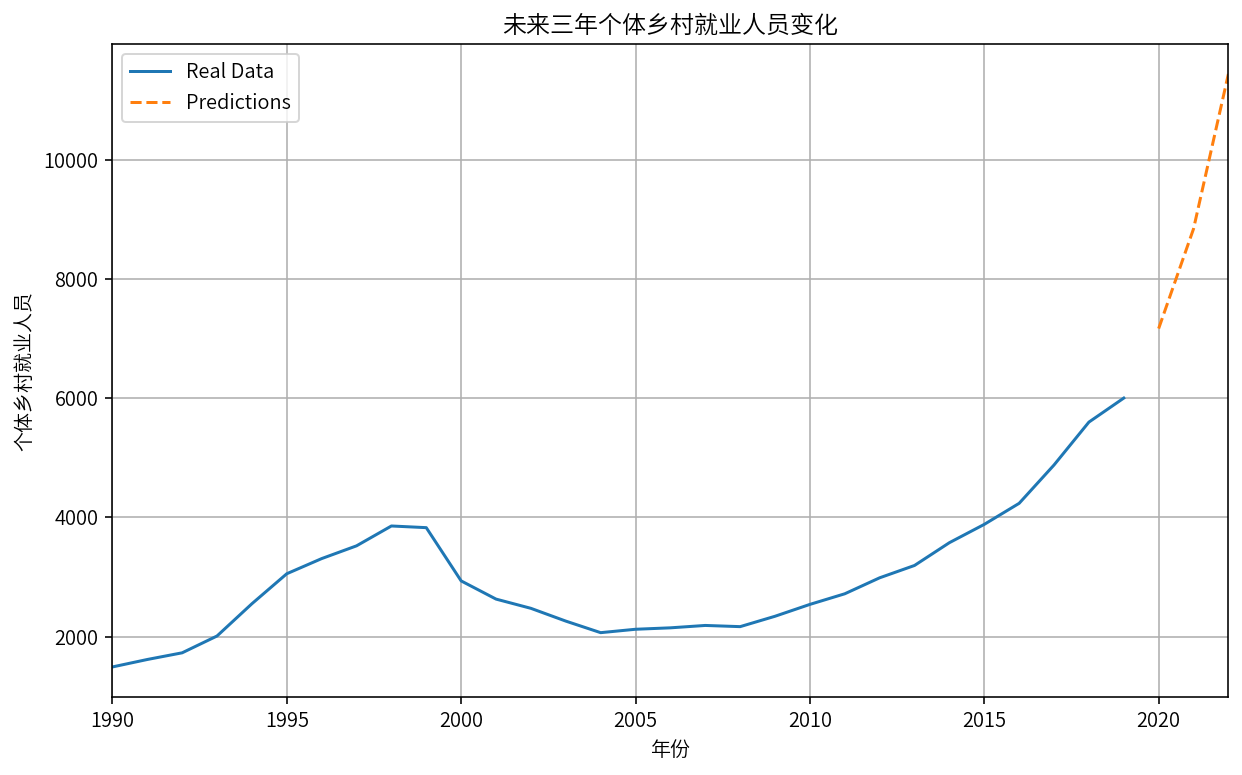
\includegraphics[width=\linewidth]{figures/24.png}
        \caption{δ��������廧����ҵ��Ա�仯ͼ}
        \label{fig:prediction_self_employed}
    \end{minipage}\hfill
    \begin{minipage}{0.45\linewidth}
        \centering
        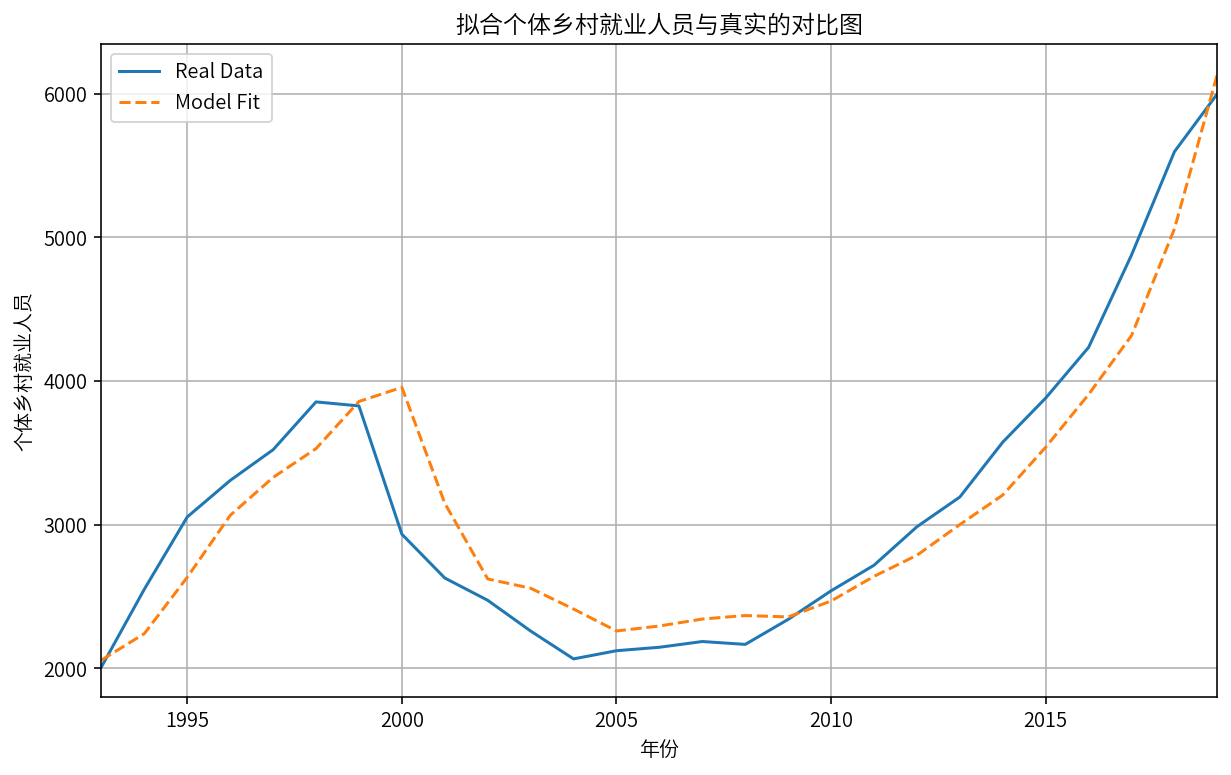
\includegraphics[width=\linewidth]{figures/25.png}
        \caption{��ϸ��廧����ҵ��Ա����ʵ�ĶԱ�ͼ}
        \label{fig:fit-vs-real_self_employed}
    \end{minipage}
\end{figure}

\begin{table}[H]
\caption{���廧����ҵ��Ա����}
\begin{subtable}{0.5\textwidth}
  \centering
  % Table 1
  \caption{��ȫ��ȱ���廧����ҵ��Ա}
  \begin{tabular}{cc}
    \hline
    \hline
    \textbf{���} & \textbf{���廧����ҵ��Ա}\\
    \hline
    2020 & 7228.06\\
    2021 & 8956.09\\
    2022 & 11552.06\\
    \hline
  \end{tabular}
\end{subtable}%
\begin{subtable}{0.5\textwidth}
  \centering
  % Table 2
  \caption{Ԥ���������廧����ҵ��Ա}
  \begin{tabular}{cc}
    \hline
    \hline
    \textbf{���} & \textbf{���廧����ҵ��Ա}\\
    \hline
    2023 & 14889.481\\
    2024 & 17813.33\\
    2025 & 19633.70\\
    \hline
  \end{tabular}
\end{subtable}

\end{table}

������Ԥ�⣬���廧����ҵ��Ա��˽Ӫ��ҵ����ҵ��Ա������ʵ�ֽϴ��������������ũҵ��ҵ�ĺ����������ڴӴ�ͳ��ʽת��Ϊ�Ը��廧��˽Ӫ��ҵΪ������

������ǰ����ͬ�ķ�������������DLF-LSTMģ�ͶԳ����ҵ��Ա���ݽ�����Ԥ�⡣����ģ�͵�ѵ������֤���õ���Ԥ��δ��ʮ������ҵ�����仯��ͼ�������ݡ�

\begin{figure}[h]
    \centering
    \begin{minipage}{0.3\linewidth}
        \centering
        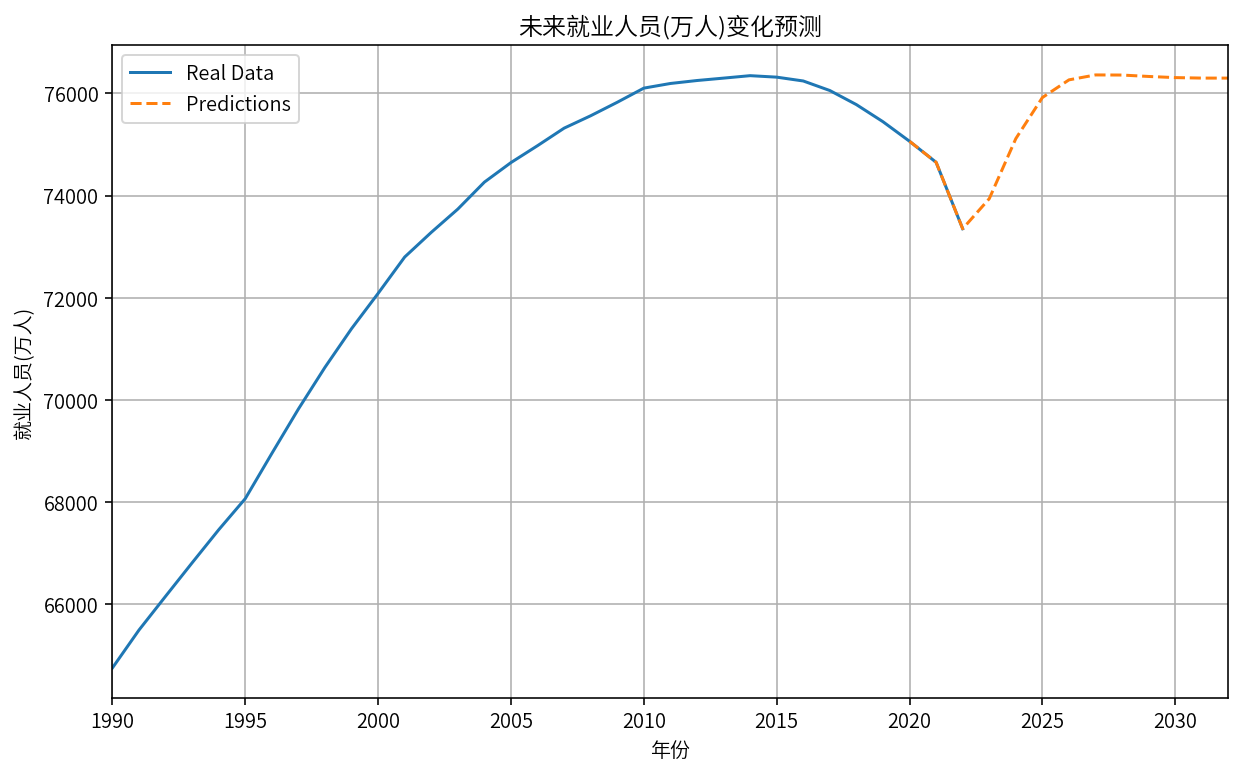
\includegraphics[width=\linewidth]{figures/26.png}
        \caption{δ����ҵ��Ա�仯Ԥ��}
        \label{fig:prediction_employment}
    \end{minipage}\hfill
    \begin{minipage}{0.3\linewidth}
        \centering
        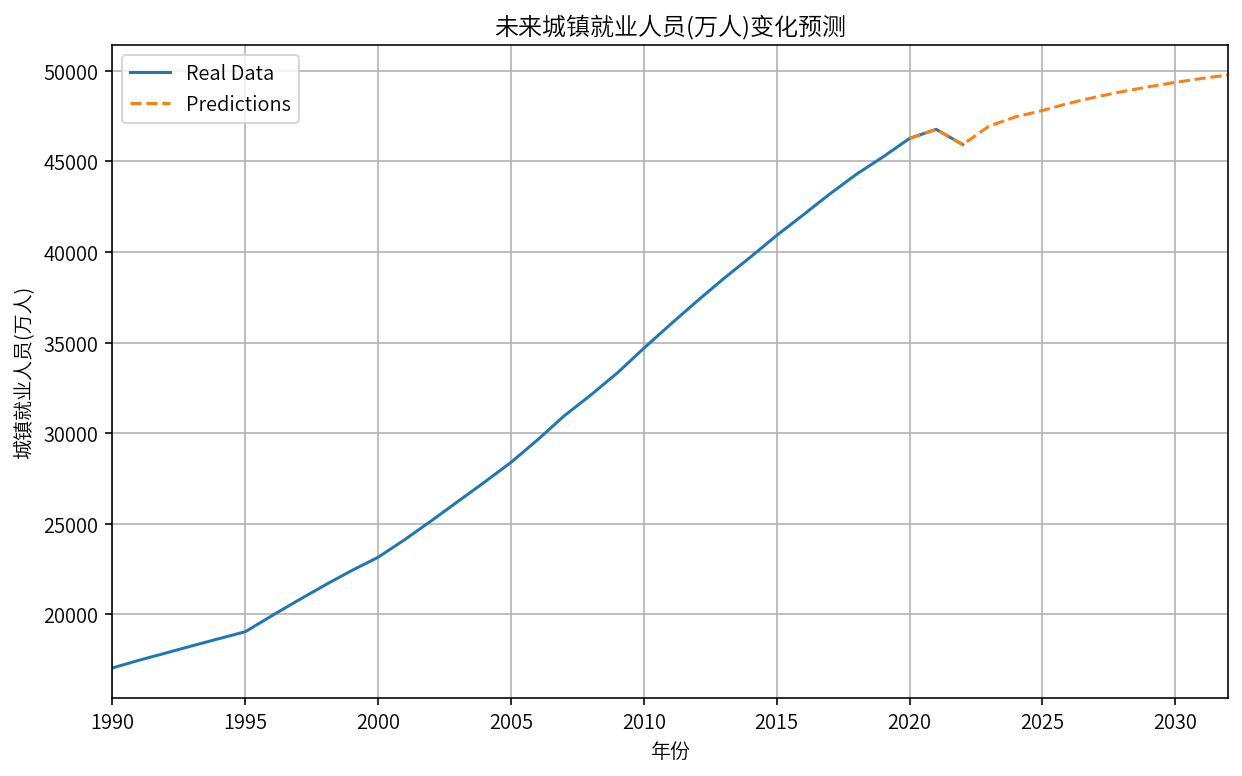
\includegraphics[width=\linewidth]{figures/27.png}
        \caption{�����ҵ��Ա�仯Ԥ��}
        \label{fig:fit-vs-real_employment_city}
    \end{minipage}\hfill
    \begin{minipage}{0.3\linewidth}
        \centering
        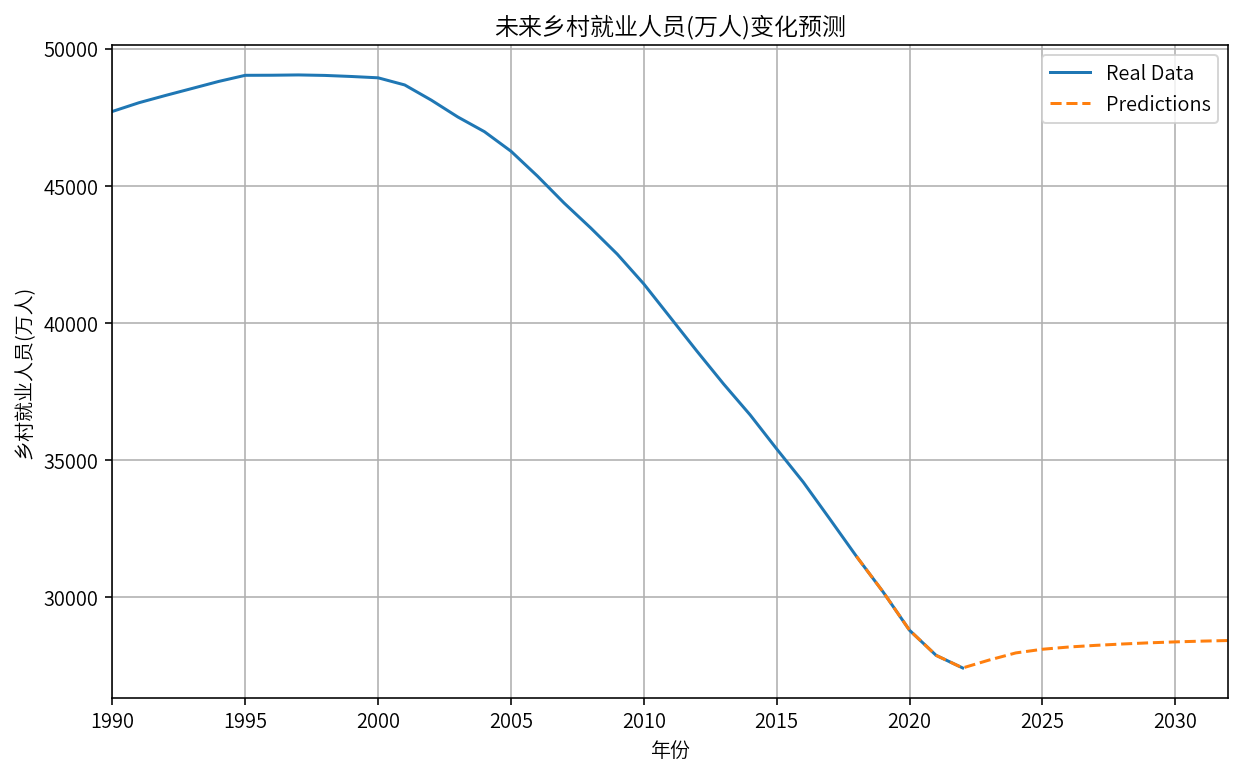
\includegraphics[width=\linewidth]{figures/28.png}
        \caption{����ҵ��Ա�仯Ԥ��}
        \label{fig:fit-vs-real_employment_village}
    \end{minipage}
\end{figure}

ͼ����ʾ�ܾ�ҵ�����ھ�����һ����������֮������ƽ�Ȳ����в�����Ԥ����ʾδ������һ���IJ�����������ά����һ�����ƽ�ȵ�ˮƽ���������ζ�ž�ҵ�г��ڴﵽһ����ģ�󣬽�����һ����Ϊ����Ľ׶Σ������ٶȷŻ���

Ԥ�Ƴ����ҵ��Ա���������������������ƣ����������ٶ��𽥷Ż�����ʾ��һ�����ȶ������ơ�����������ҵ�г��ķ�չ�Ѿ���������죬δ�����������ܸ�����ܵ��������ں����ߵ��ص�Ӱ�졣

\begin{table}[h]
    \centering
    \begin{minipage}{0.32\linewidth}
        \centering
        \caption{Ԥ���ҵ��Ա�仯}
        \label{tab:total_employment}
        \begin{tabular}{cc}
        \hline
        ��� & Ԥ���ҵ��Ա(����) \\
        \hline
        2020 & 73939.57 \\
        2021 & 75116.24 \\
        2022 & 75921.16 \\
        2023 & 76266.91 \\
        \hline
        \end{tabular}
    \end{minipage}\hfill
    \begin{minipage}{0.32\linewidth}
        \centering
        \caption{�����ҵ��Ա�仯Ԥ��}
        \label{tab:urban_employment}
        \begin{tabular}{cc}
        \hline
        ��� & Ԥ������ҵ��Ա(����) \\
        \hline
        2020 & 46958.44 \\
        2021 & 47466.87 \\
        2022 & 47811.33 \\
        2023 & 48213.55 \\
        \hline
        \end{tabular}
    \end{minipage}\hfill
    \begin{minipage}{0.32\linewidth}
        \centering
        \caption{����ҵ��Ա�仯Ԥ��}
        \label{tab:rural_employment}
        \begin{tabular}{cc}
        \hline
        ��� & Ԥ������ҵ��Ա(����) \\
        \hline
        2018 & 27709.54 \\
        2019 & 27967.95 \\
        2020 & 28101.58 \\
        2021 & 28183.98 \\
        \hline
        \end{tabular}
    \end{minipage}
\end{table}


ũ���ҵ��Ա����Ԥ���ڳ�ʼ�׶���ʾ�½����ƣ����תΪƽ�������������ơ�����ܷ�ӳ������ũҵ�Զ����͹�ҵ�����ƽ���ũ���Ͷ���������٣�����������֧�ֺ�ũ�徭�ýṹ���𲽵�����ũ���ҵ�����������ȶ���������������ơ�

\section{��֧������}
ũ������ˮƽ������������ũ���֧������Ļ����ϣ���֧������ֱ��Ӱ�쵽ũ�������������ֻ�е�ũ��ӵ���㹻�Ŀ�֧������ʱ�����Dz��ܹ�������������ͥ�����������������������������ʺ��Ļ����󣬽����ƶ�ũ��������������뷱�١�

% �����ռ���2016����2023���ڼ��ũ���֧���������ݣ��Դ�Ϊ������������Ӧ������ͼ������ͼ��ʾ��

% \begin{figure}[h]
%     \centering
%     \begin{subfigure}{0.5\textwidth}
%         \centering
%         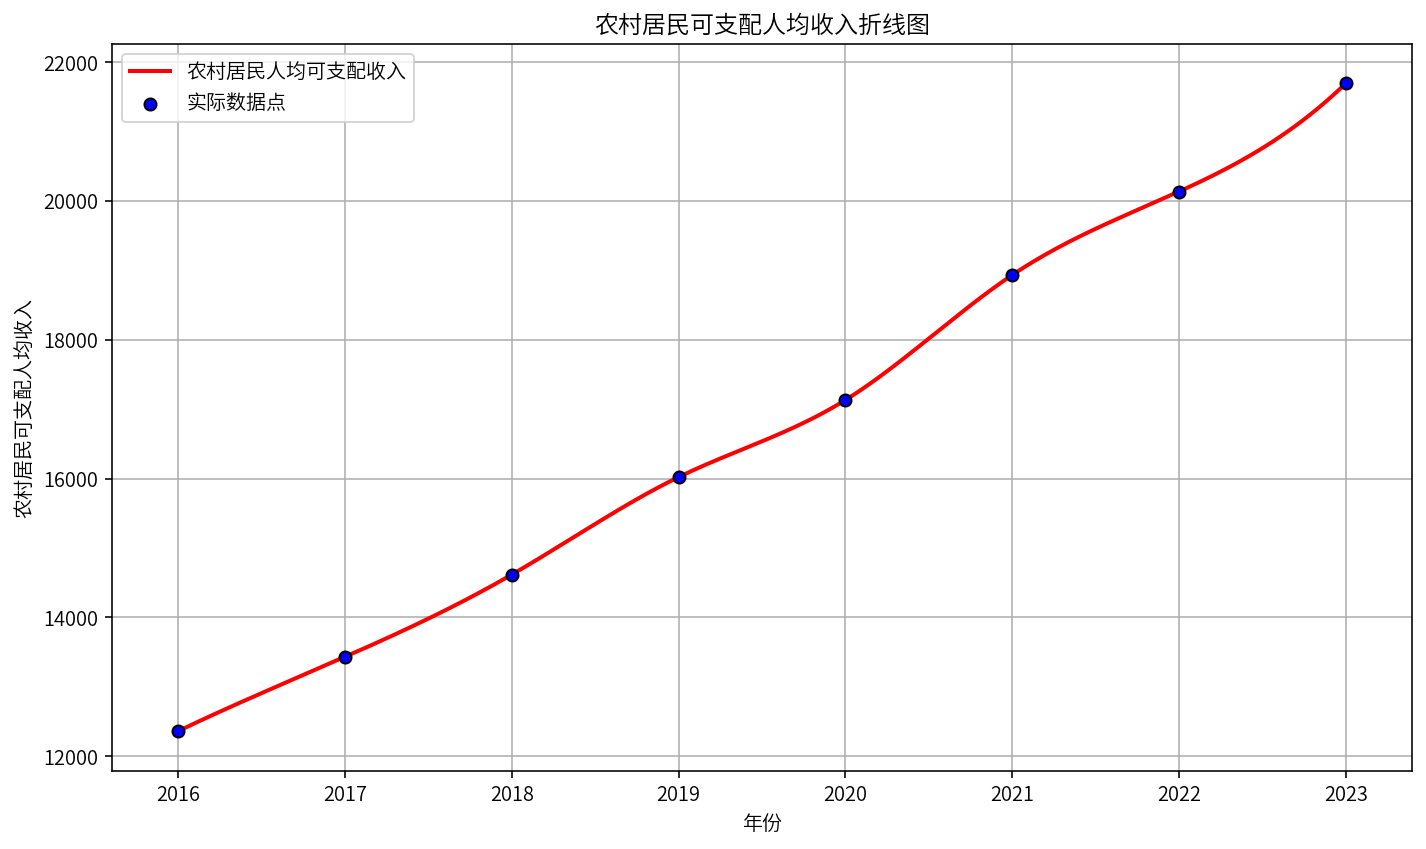
\includegraphics[width=\linewidth]{figures/39.png}
%         \caption{ũ���֧����������ͼ}
%         \label{fig:sub1}
%     \end{subfigure}%
%     \begin{subfigure}{0.5\textwidth}
%         \centering
%         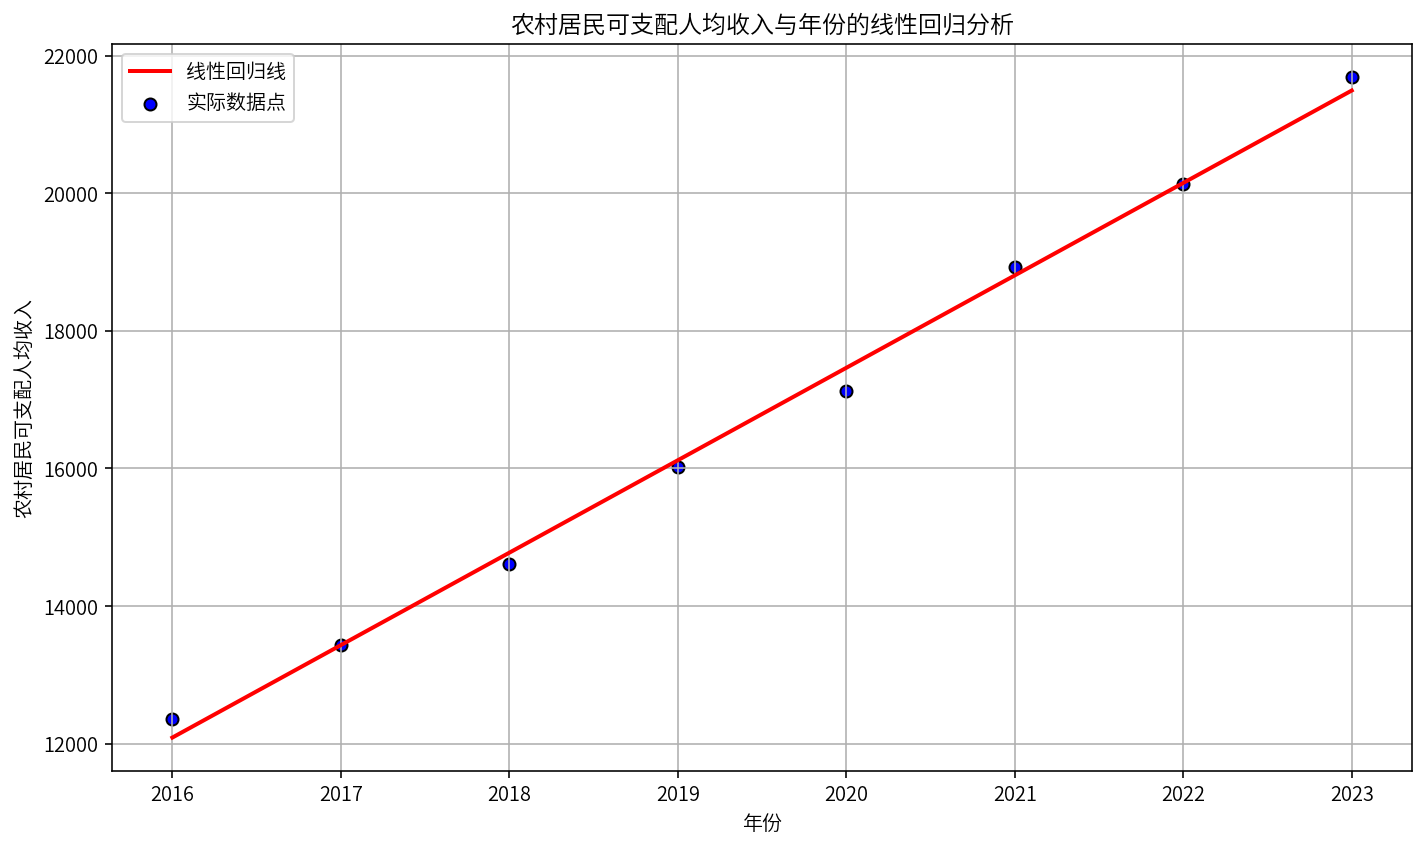
\includegraphics[width=\linewidth]{figures/38.png}
%         \caption{ũ���֧�������������ͼ}
%         \label{fig:sub2}
%     \end{subfigure}
%     \caption{ũ���֧������ͼ}
%     \label{fig:combined}
% \end{figure}


% ͼ5.9�����ʾ��ũ��Ŀ�֧�����������ȶ����������������мӿ�ļ���������ֳ��������ơ�����������һ�µ��������ƣ�û�������������µ������󣬱����ڹ�ȥ�����У�ũ��ľ���״���ȶ���á��ⲻ��Ԥʾ��ũ������ˮƽ���ձ�������Ҳ��ӳ��ũ�徭�÷�չ���߿��ܵ�����Ч����

������ϸ��ಢ�����˴�1999����2022��䣬�й�ũ���������Ŀ�֧������������֧����ȫ�����ݼ����о��ĺ�����������˹Ƥ�����ȼ����ϵ����һǿ�����ķDz���ͳ�ƹ��ߣ��÷�������������ݷ����ض��ֲ���������Ч���������������Ƿ���ڵ���������ݼ��Ĺ�ϵ��
ͨ���������¹�ʽ
\begin{equation}
\rho = 1 - \frac{6 \sum d_i^2}{n(n^2 - 1)}
\hspace{1em}
\footnote{���� \(\rho\) ������س̶ȣ�\(d_i\) Ϊÿһ�Թ۲�ֵ�ڸ��������֮��� \(n\) ������������}
\end{equation}

��������̽����������֧��������DZ�ڵĹ���ģʽ�����������ʾ�������ͼ�������ؽ�ʾ��ũ������֧��������������֧��֮����ڼ�Ϊ��������������������ơ�
\begin{figure}[H]
    \centering
    \begin{subfigure}{0.5\textwidth}
        \centering
        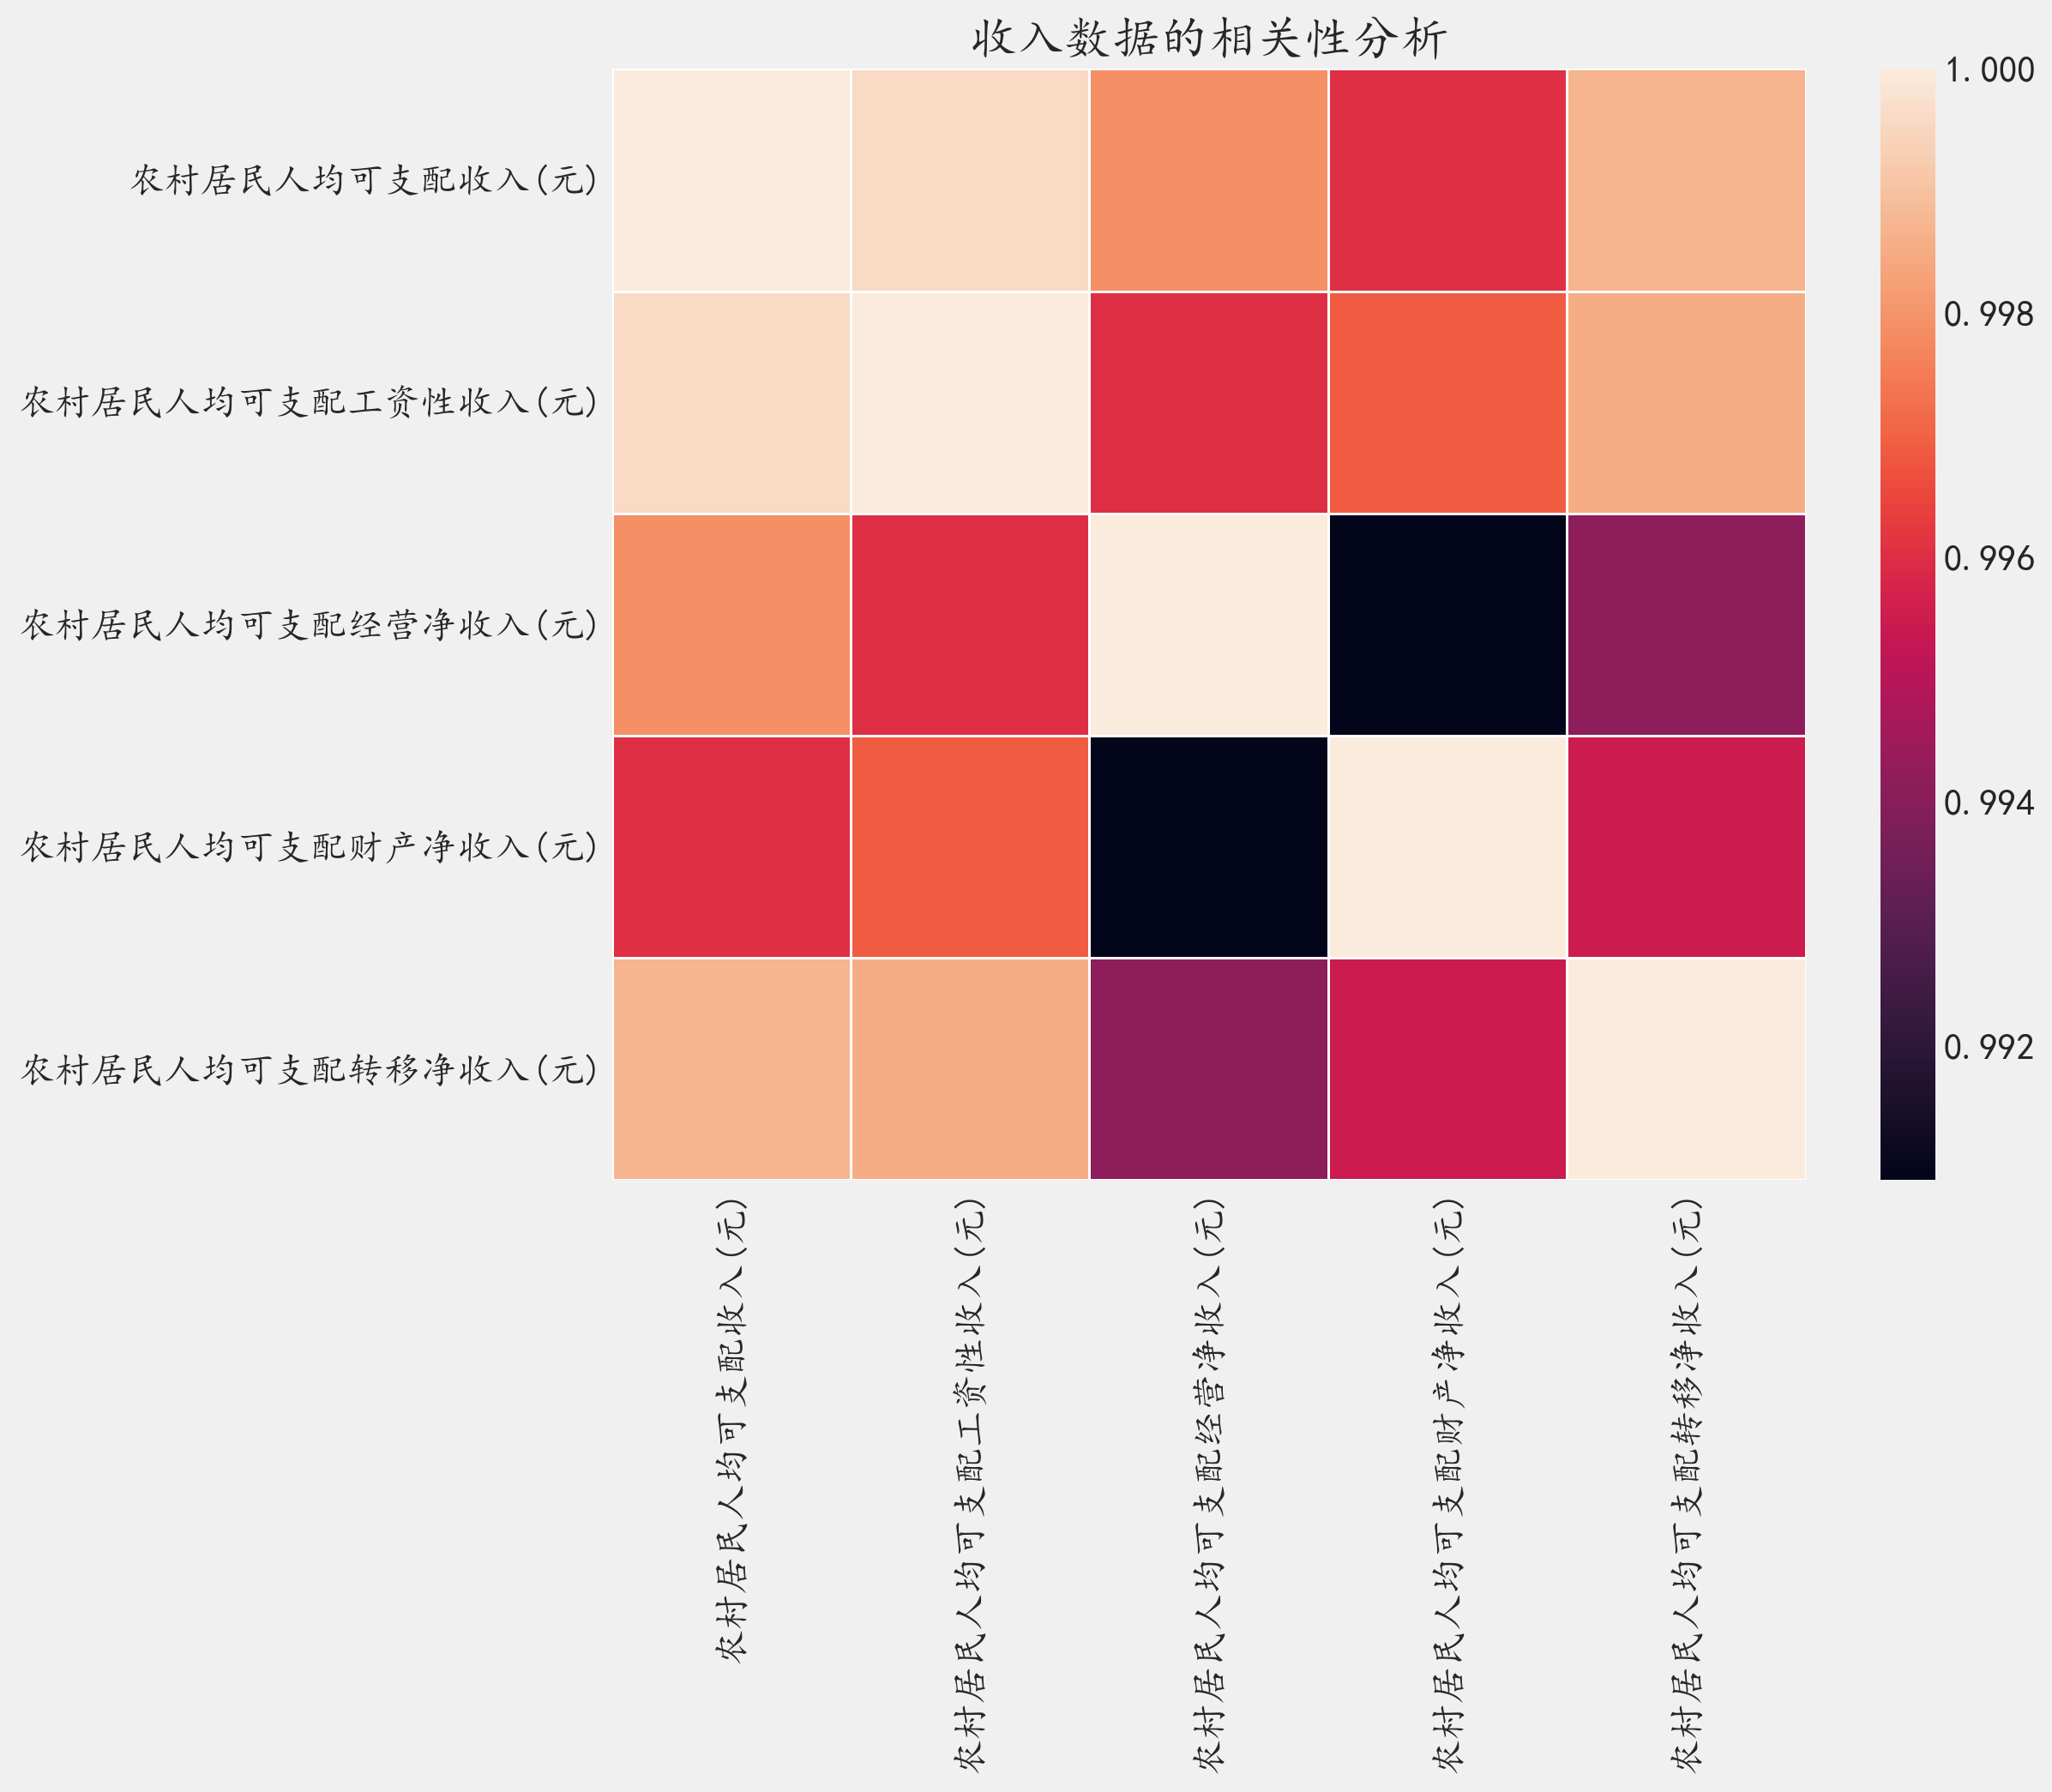
\includegraphics[width=\linewidth]{figures/income_corr.png}
        \caption{�������ݵ�����Է���}
        \label{fig:income_corr}
    \end{subfigure}
    \begin{subfigure}{0.49\textwidth}
        \centering
        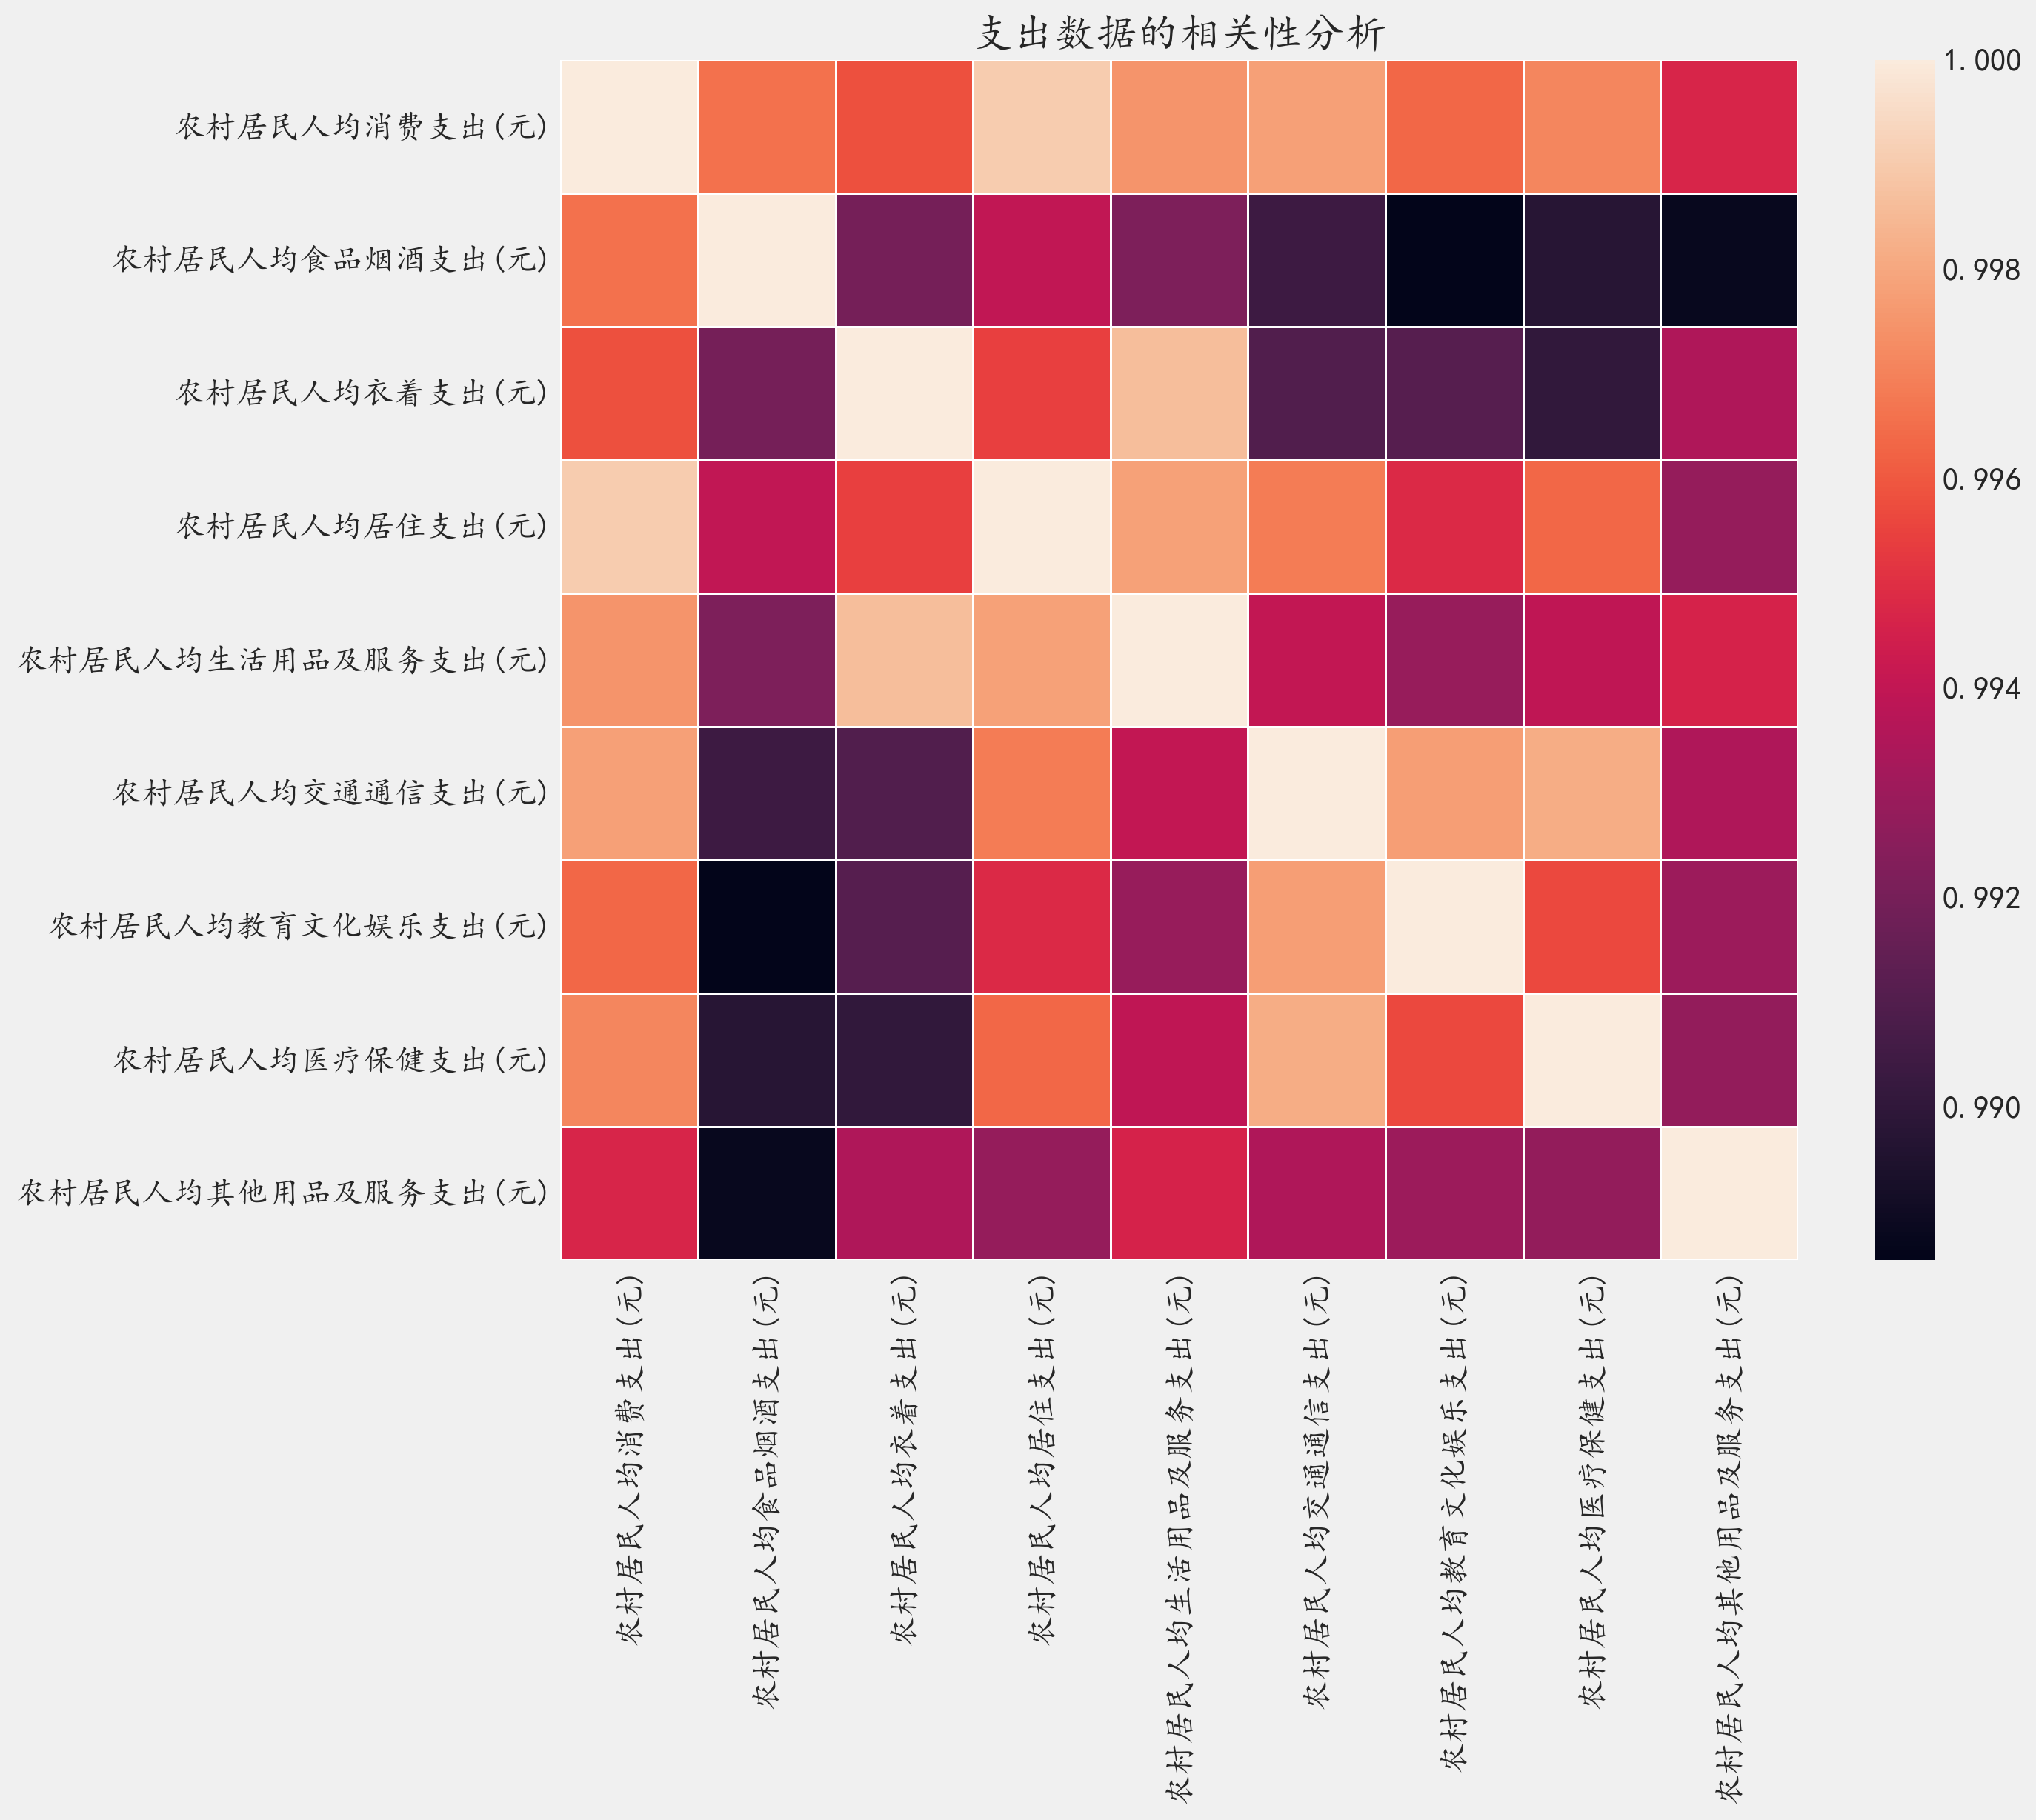
\includegraphics[width=\linewidth]{figures/expenditure_corr.png}
        \caption{֧�����ݵ�����Է���}
        \label{fig:expenditure_corr}
    \end{subfigure}
    \caption{˹Ƥ�����ȼ����ϵ������ͼ��}
\end{figure}

Ϊ��һ������⣬���о���ȡ�����ɷַ�����PCA������������һ��ǿ��Ľ�ά�ֶΣ�ּ�ڴӸ��ӵ����ݼ�����������߽��������ۺ�ָ�ꡣPCAͨ����ԭʼ����ת�����µ�����ϵͳ�У������ɷַ����ϣ������ܽ������ݷ���ķ�ʽ���±������ݣ����������������������������ԣ�����Ԥ�������������ݵ����Ļ��ͱ�׼��������ء�����õ�PCAͼ������չ����������֧����������ά���ϵĽṹ�����������ڽ�ʾ���ص�ģʽ�ͼ���������Ϣ��

\begin{figure}[H]
    \centering
    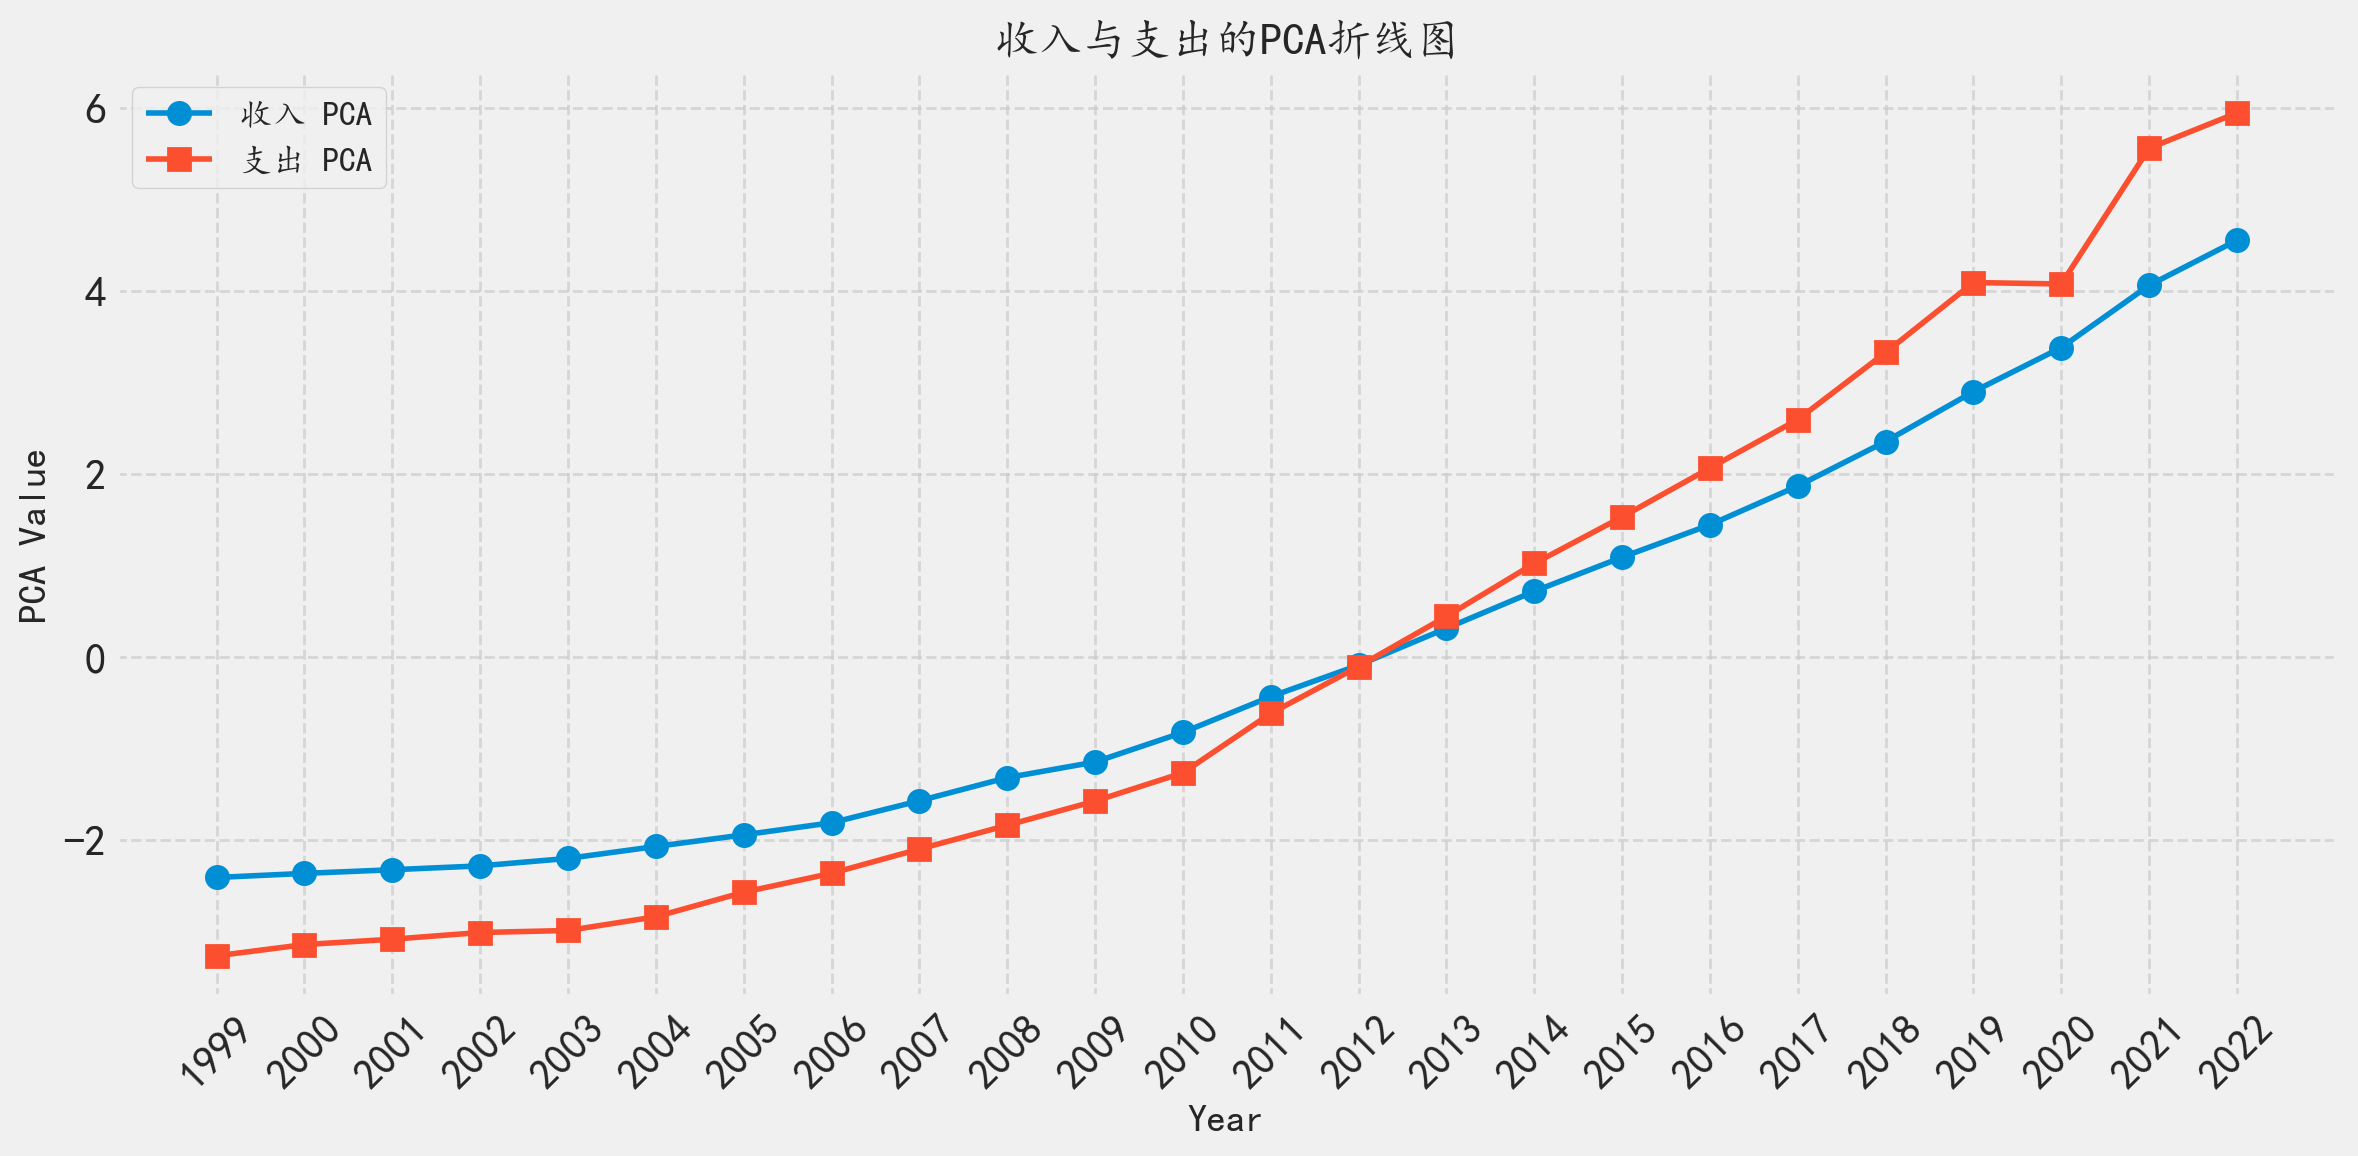
\includegraphics[width=0.75\linewidth]{figures/PCA.png}
    \caption{���ɷַ���ͼ��}
    \label{fig:PCA}
\end{figure}

�ڴ˻����ϣ����Dz���ţ�ٶ�Ԫ��ִ�з����Իع��������ģ�� \(a * x^2 + b * x + c\) ����ũ���������������֧����ʱ��仯�Ķ�̬���ɣ��ɹ�������������ߡ���һ���ֲ������������Ƕ�ũ�徭�û�����Ժͳ������Ƶ����⣬ҲΪ�����ƶ����ṩ�˱�����������ݡ�

\begin{figure}[H]
    \centering
    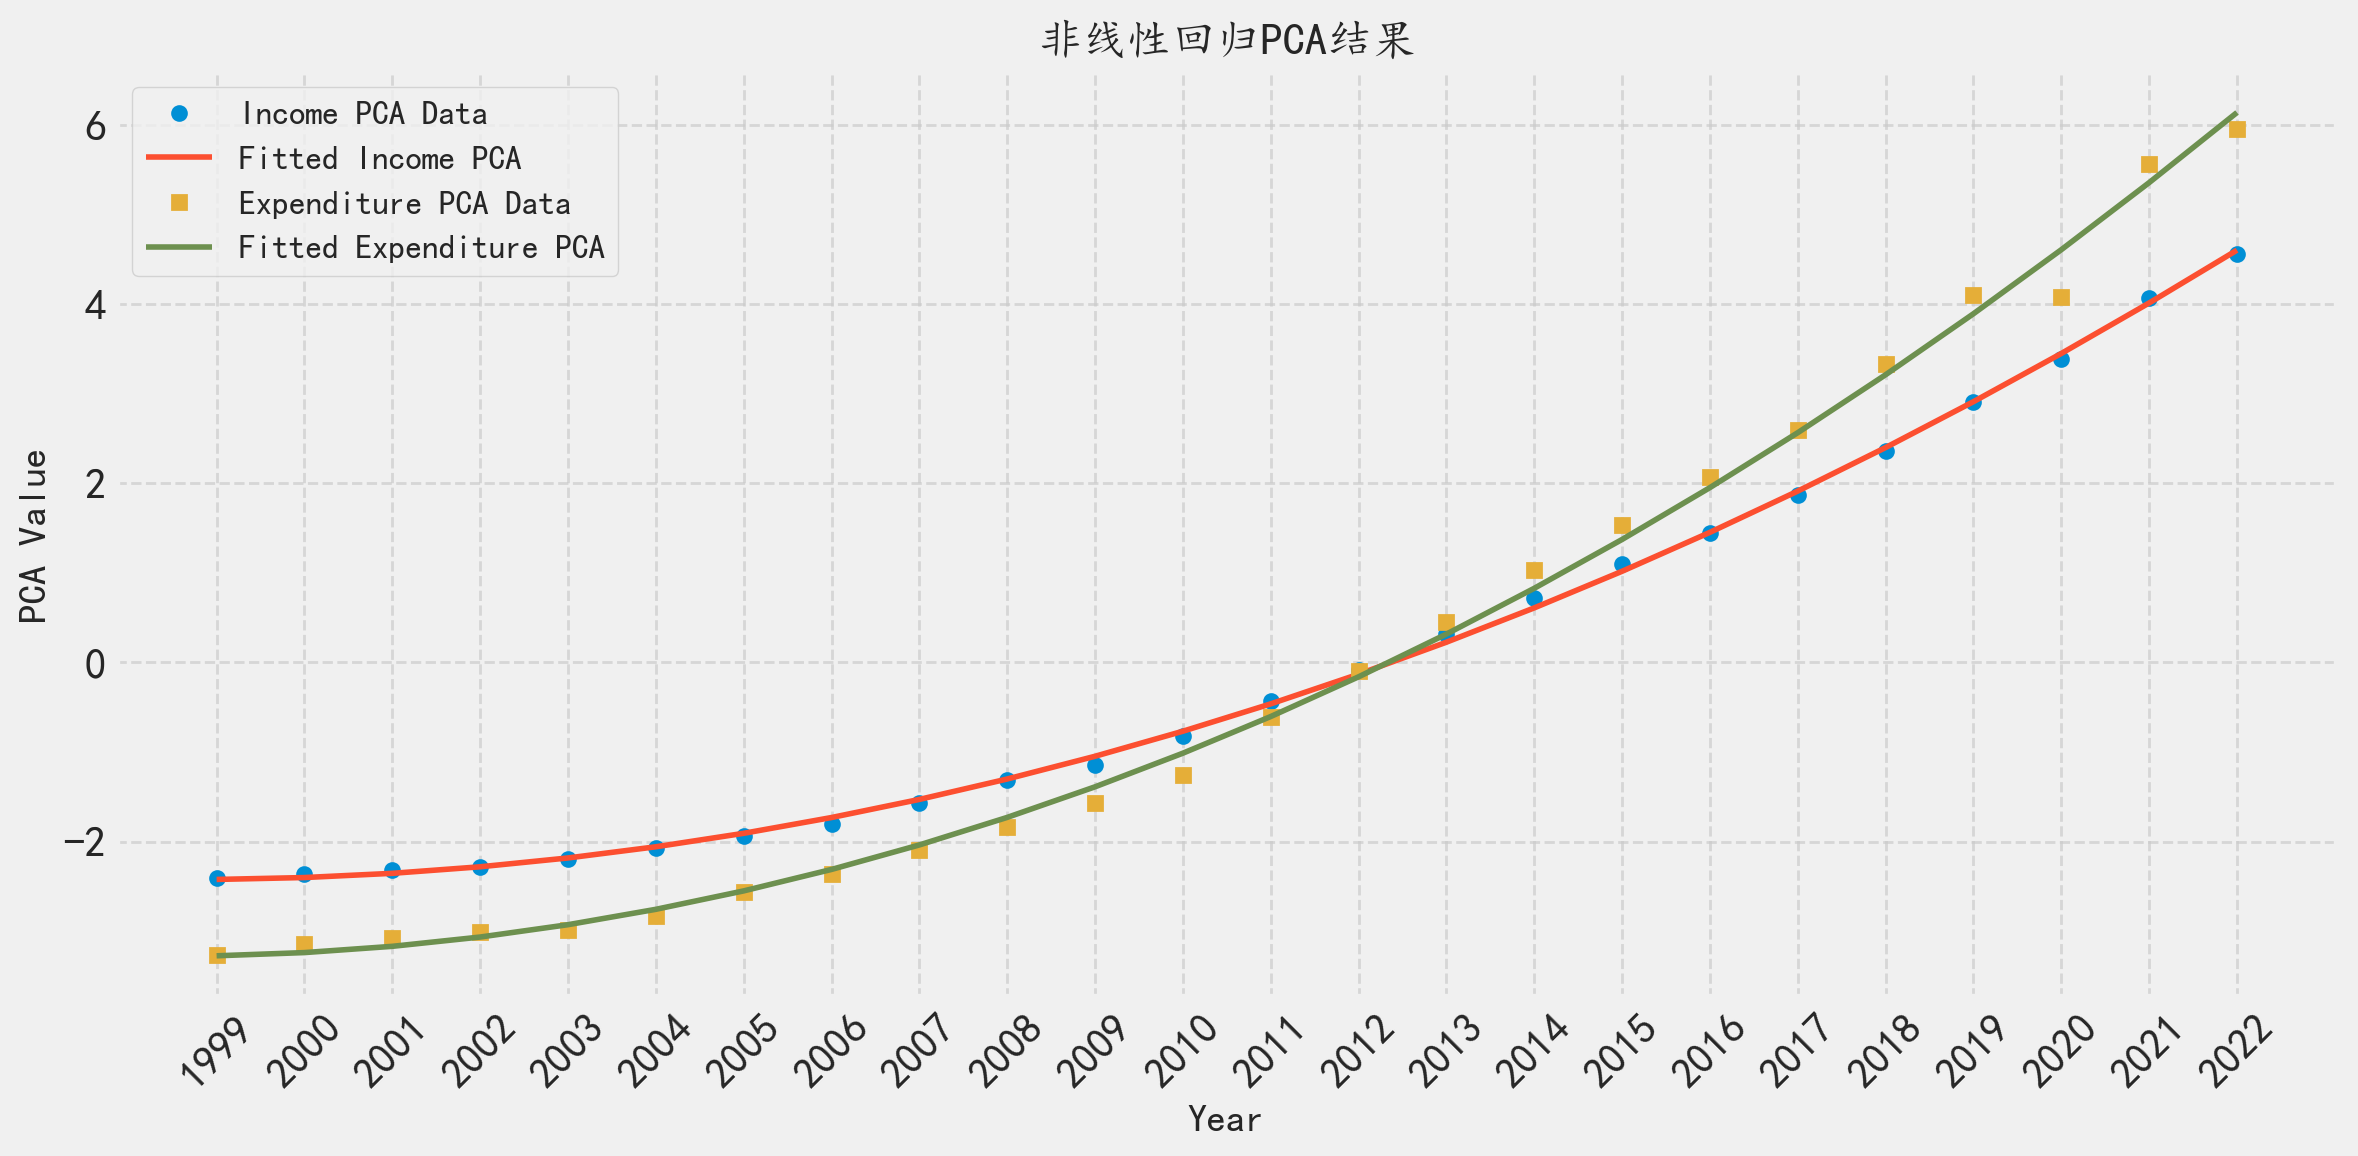
\includegraphics[width=0.75\linewidth]{figures/poly_PCA.png}
    \caption{�����Իع�PCA���}
    \label{fig:poly_PCA}
\end{figure}

���ͨ���Ա�ƽ��������ƽ������֧�����������ͼ���о���ʾ��һ�����˹�ע�����ƣ����߼�IJ������ʱ�����ƶ���������͹����ũ�徭�÷�չ�������������Ӹ�ԣ���������ƶ���׼��Ч�����ߴ�ʩ���ٽ�ũ�徭�õľ��ⷢչ������ũ����������ˮƽ���׿Խ��Ч��

\begin{figure}[H]
    \centering
    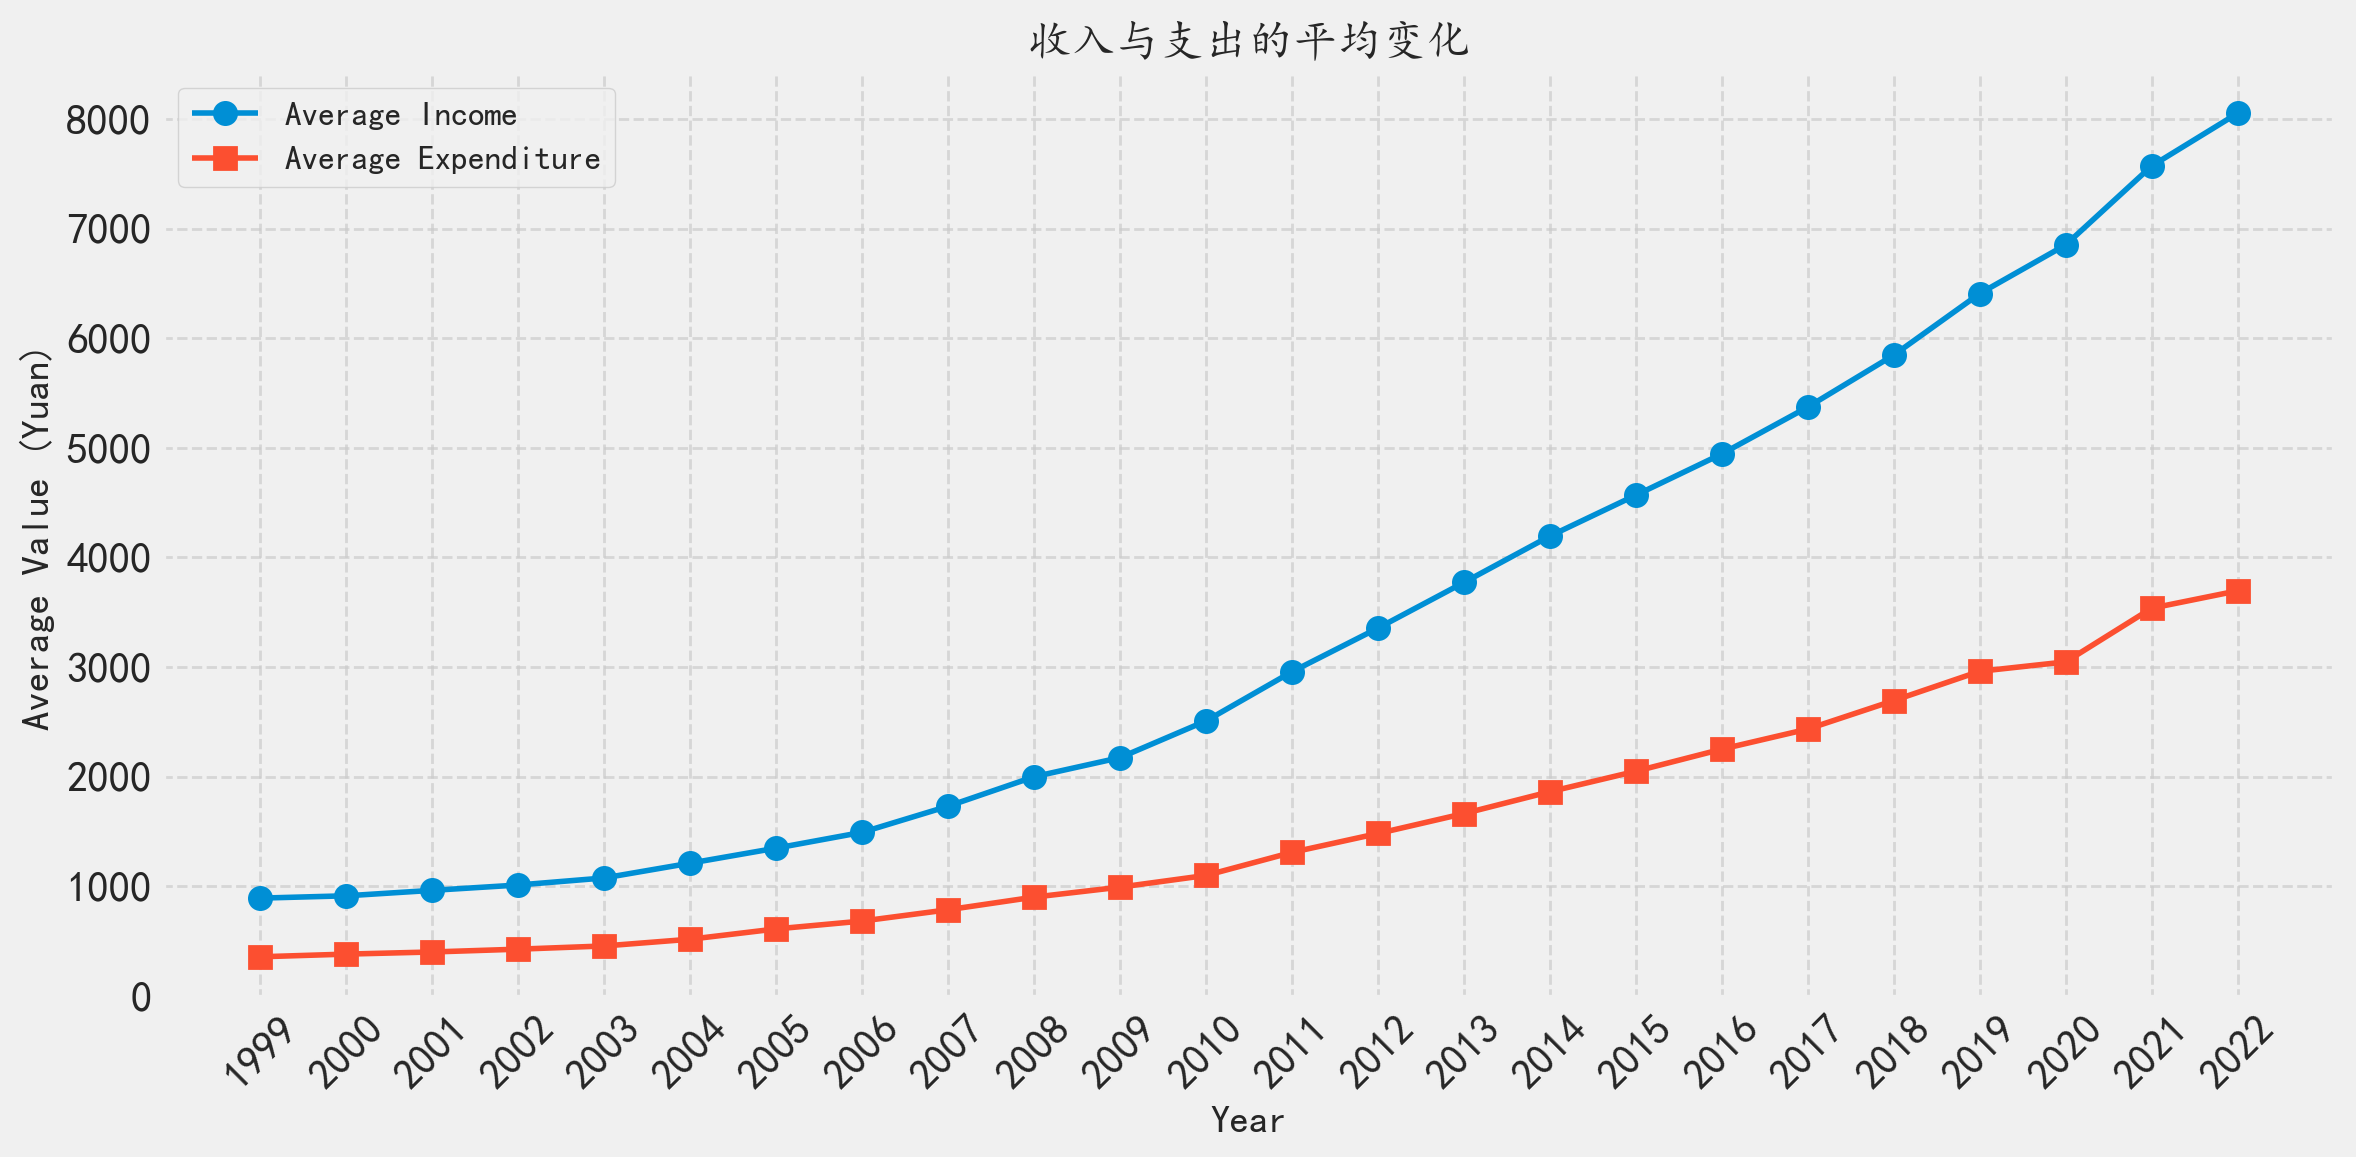
\includegraphics[width=0.75\linewidth]{figures/average_change.png}
    \caption{����֧��ƽ���껯����ͼ}
    \label{fig:average_change}
\end{figure}

\section{��������}

������������֧����������ӡ��Ƽ���Ѹ�ٽ����Լ����ߵĻ����ƶ��£�������������������������ڲ��������Ĺ켣֮�ϡ�Ϊ�����������һ�仯�����Dzɼ��������˹�����Ҫ��ͨ���ߺͻ������õ�����ӵ�������ݣ��Ա��˹�ȥʮ���뵱ǰ����µ����ݻ������״�ͼ��

\begin{figure}[H]
    \centering
    \begin{minipage}{0.43\textwidth}
        \centering
        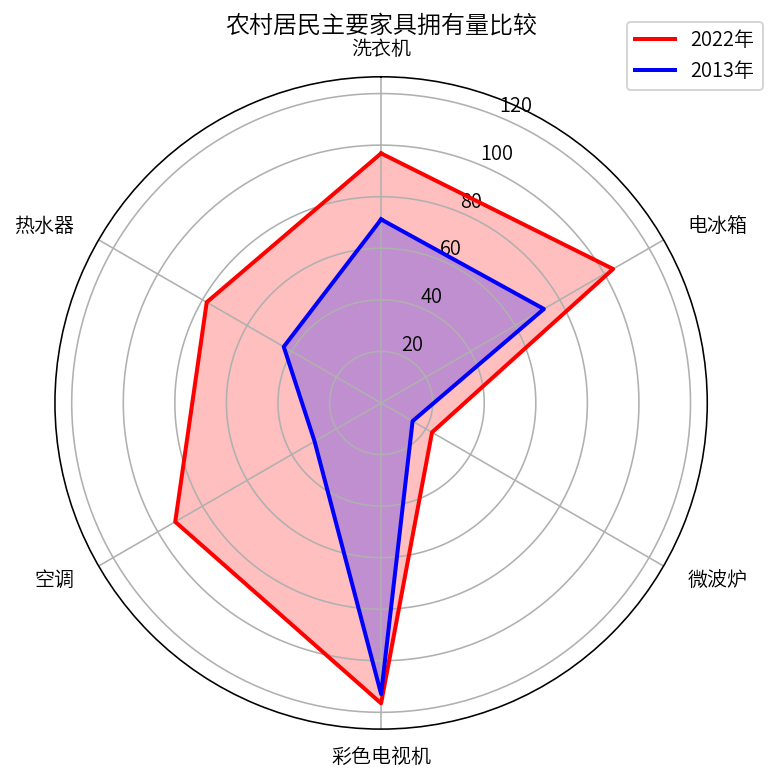
\includegraphics[width=\linewidth]{figures/43.png}
        \caption{ũ�������Ҫ�Ҿ�ӵ�����Ƚ�}
        \label{fig:furniture}
    \end{minipage}\hfill
    \begin{minipage}{0.43\textwidth}
        \centering
        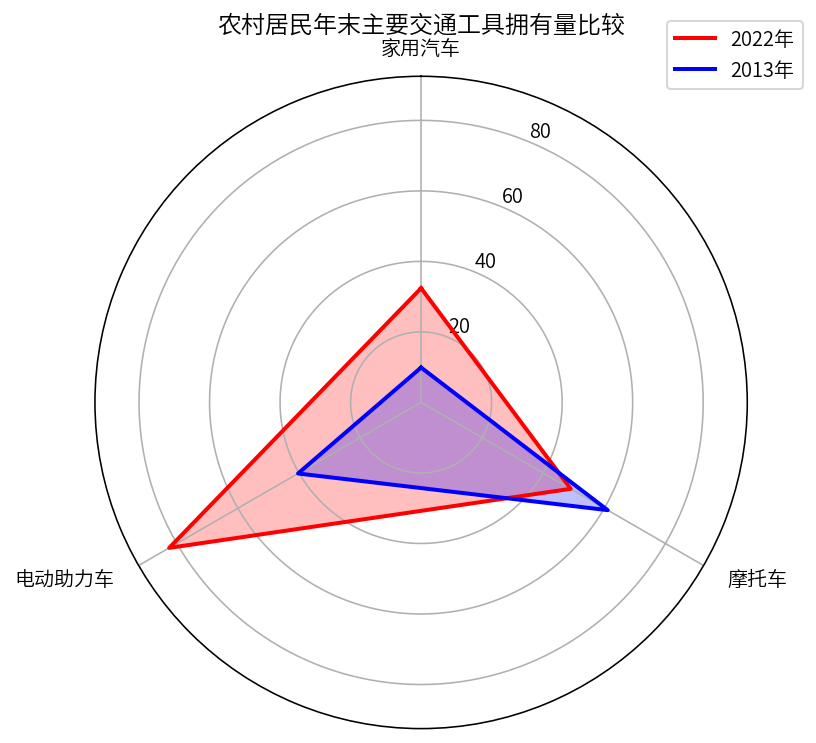
\includegraphics[width=\linewidth]{figures/44.png}
        \caption{ũ�������ĩ��Ҫ��ͨ����ӵ�����Ƚ�}
        \label{fig:vehicles}
    \end{minipage}
\end{figure}


ͨ��ϸ�¹������״�ͼ������ֱ�Ӷ��쵽ϴ�»�������䡢΢��¯����ɫ���ӻ����յ��Լ���ˮ���Ȼ����ҵ��ӵ�����������ӣ���һ�仯͹��������������ˮƽ�����������������ĸ��ơ���ͨ�����У���Ħ�г��ܵ����߱䶯��Ӱ��������½����ƣ����������͵綯������ʵ���������������ⲻ����ӳ����������ͨ����ʹ��ģʽ�ı仯��Ҳͻ�����ִ��������ж��ڱ�ݽ�ͨ��ʽ��������������

\section{�Ҹ�ָ��}

������˹�����������ۣ��˵�����ӵ͵��߷�Ϊ�������󡢰�ȫ������������������������ʵ����������ˮƽ��������Ӧ���������ʲ���ķḻ����Ӧ���������������㡣

���У������ϵ��������ͥʳƷ֧��ռ������֧���ı��أ��Ƿ�ӳ��������ˮƽ����Ҫ����ָ�ꡣ��ϵ��Խ�ͣ�������ͥ��ʳƷ�ϵ�֧��ռ��ԽС��һ����ԣ���ͥ������ˮƽԽ�ߡ�

�����Ѽ����Ըĸ↑�����������ȫ�����񣨰�������������񣩵Ķ����ϵ������\cite{china-engel-coefficients}�����ݴ˻����˷�ӳȫ�������Լ�ũ���������ϵ���仯������ͼ������ͼ��ʾ��

\begin{figure}[H]
    \centering
    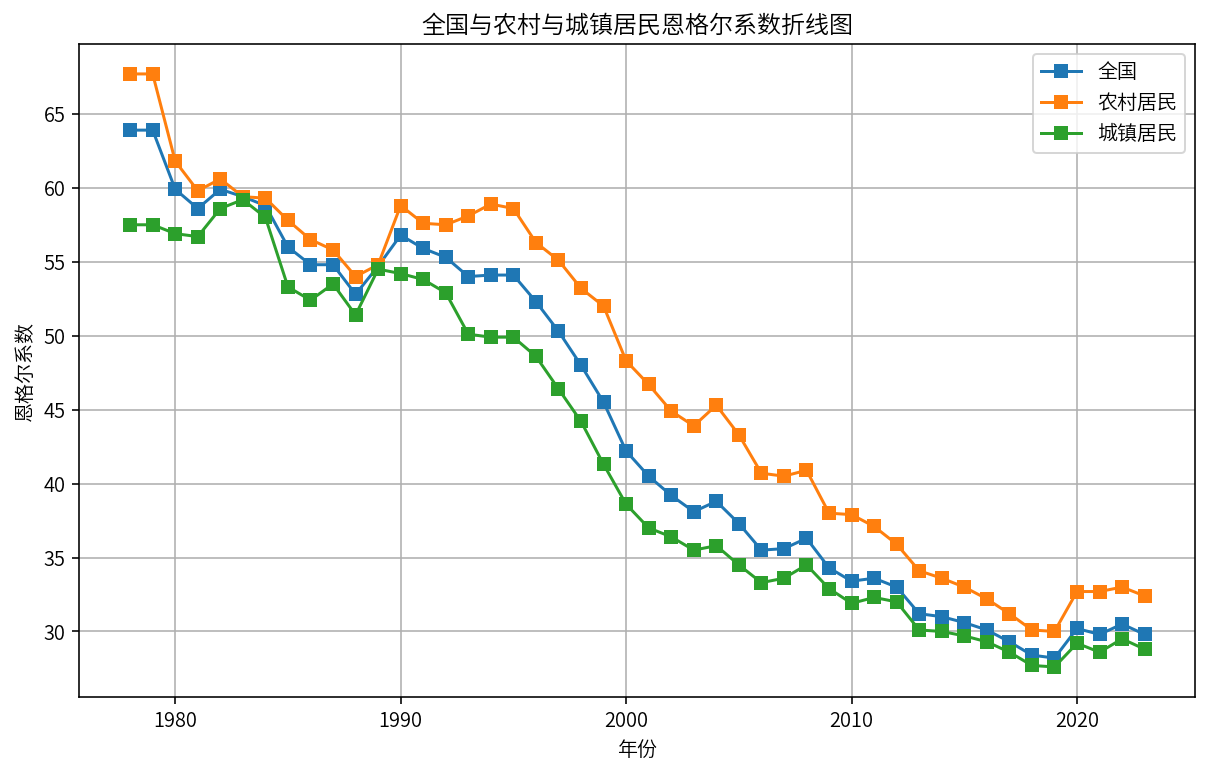
\includegraphics[width=0.65\linewidth]{figures/29.png}
    \caption{ũ����������ϵ������ͼ}
    \label{fig:Engel_coefficient_village}
\end{figure}

ͼ\ref{fig:Engel_coefficient_village}����ؽ�ʾ�˹�ȥ��ʮ����ҹ��������ѽṹ�������仯��ȫ������Ķ����ϵ�������½����ƣ���ӳ�����ž��õij�����չ����������ˮƽ������ߣ���������ѽṹ���ڷ�����̱仯���ⲻ�������˾�����������������������Ҳ��ӳ������ģʽ�Ķ�Ԫ���Ͳ�ε�������

�ر�ֵ�ù�ע���ǣ�ũ���������ϵ���������½���͹����ũ��������ѽṹ���ش�ת�䡣ũ���������Ѳ��پ����ڻ�����ʳƷ֧�������Ǹ�����������ҽ�ơ����ֵ�������չ���⣬�����������ϵ��֮��IJ���Ҳ���𽥼�С����һ���󲻽���ʾ�˳����������ˮƽ���𲽽ӽ���Ҳ��ӳ���ҹ����ƶ�����һ�廯��չ����С���緢չ��෽��ȡ�õĻ�����չ��
\chapter{�����˿ڽṹ}
\label{chapter:people}

��ͼչʾ��ȫ���˿ڽṹ���긴�������ʱ仯���������ͼ�п��Եó�������Ҫ�۲��������ȣ�ȫ�򷢴���ҵ��긴�������ʽӽ����㣬����չ�й��ҵ��긴��������ͨ����1��3֮�䣬���޵Ȳ�������ҵ��긴���������򳣳���5\%�Ҳ����ϴ���Σ����й������ķ�չ�й�����ͼ����ʾΪ����ɫ���뷢������γɶԱȣ���ʾ����޴�ķ�չDZ������δ�ȶ����˿ڽṹ��������ˣ���չũ�������Ϊ��ǰ����Ҫ��չĿ��֮һ��

\begin{figure}[H]
    \centering
    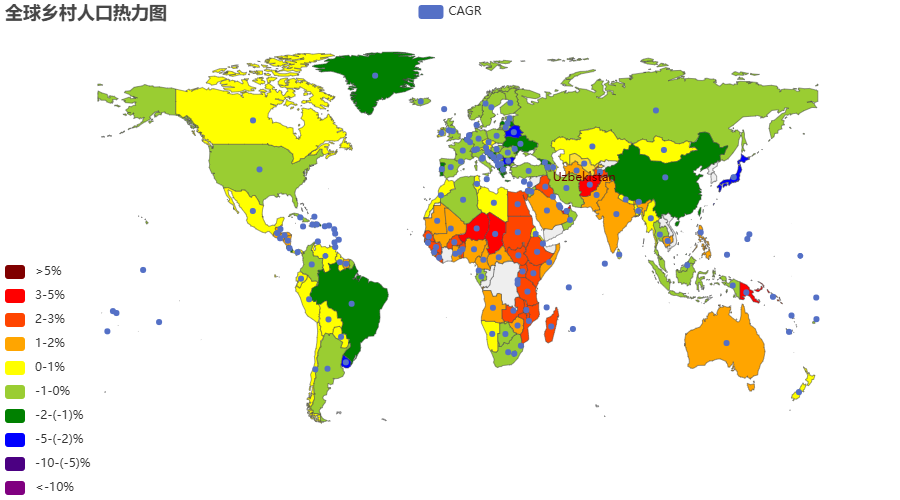
\includegraphics[width=1\linewidth]{pictures/image.png}
    \caption{ȫ������˿�����ͼ}
    \label{fig:enter-label}
\end{figure}



�Ըĸ↑���������й�ũ���������Ͷ�������д���������������һ��������������˿����仯���Ͷ�����ʧ�����⡣ΪӦ����Щ��ս����������������ս�ԣ�ּ��ͨ�����ũҵЧ�ʡ����ƻ�����ʩ�͹��������Դ�������ũ������ˮƽ���Ӷ��ٽ�ũ�徭�����ȫ�淢չ��

�����������ս�Ե�ʵʩ������˿ڽṹ�����±仯�����ǽ�����1990����2022���ÿ����������ݣ�����һϵ�б�ͼ��չʾ�й������˿ں�����˿ڵı�����

\begin{figure}[H]
    \centering
    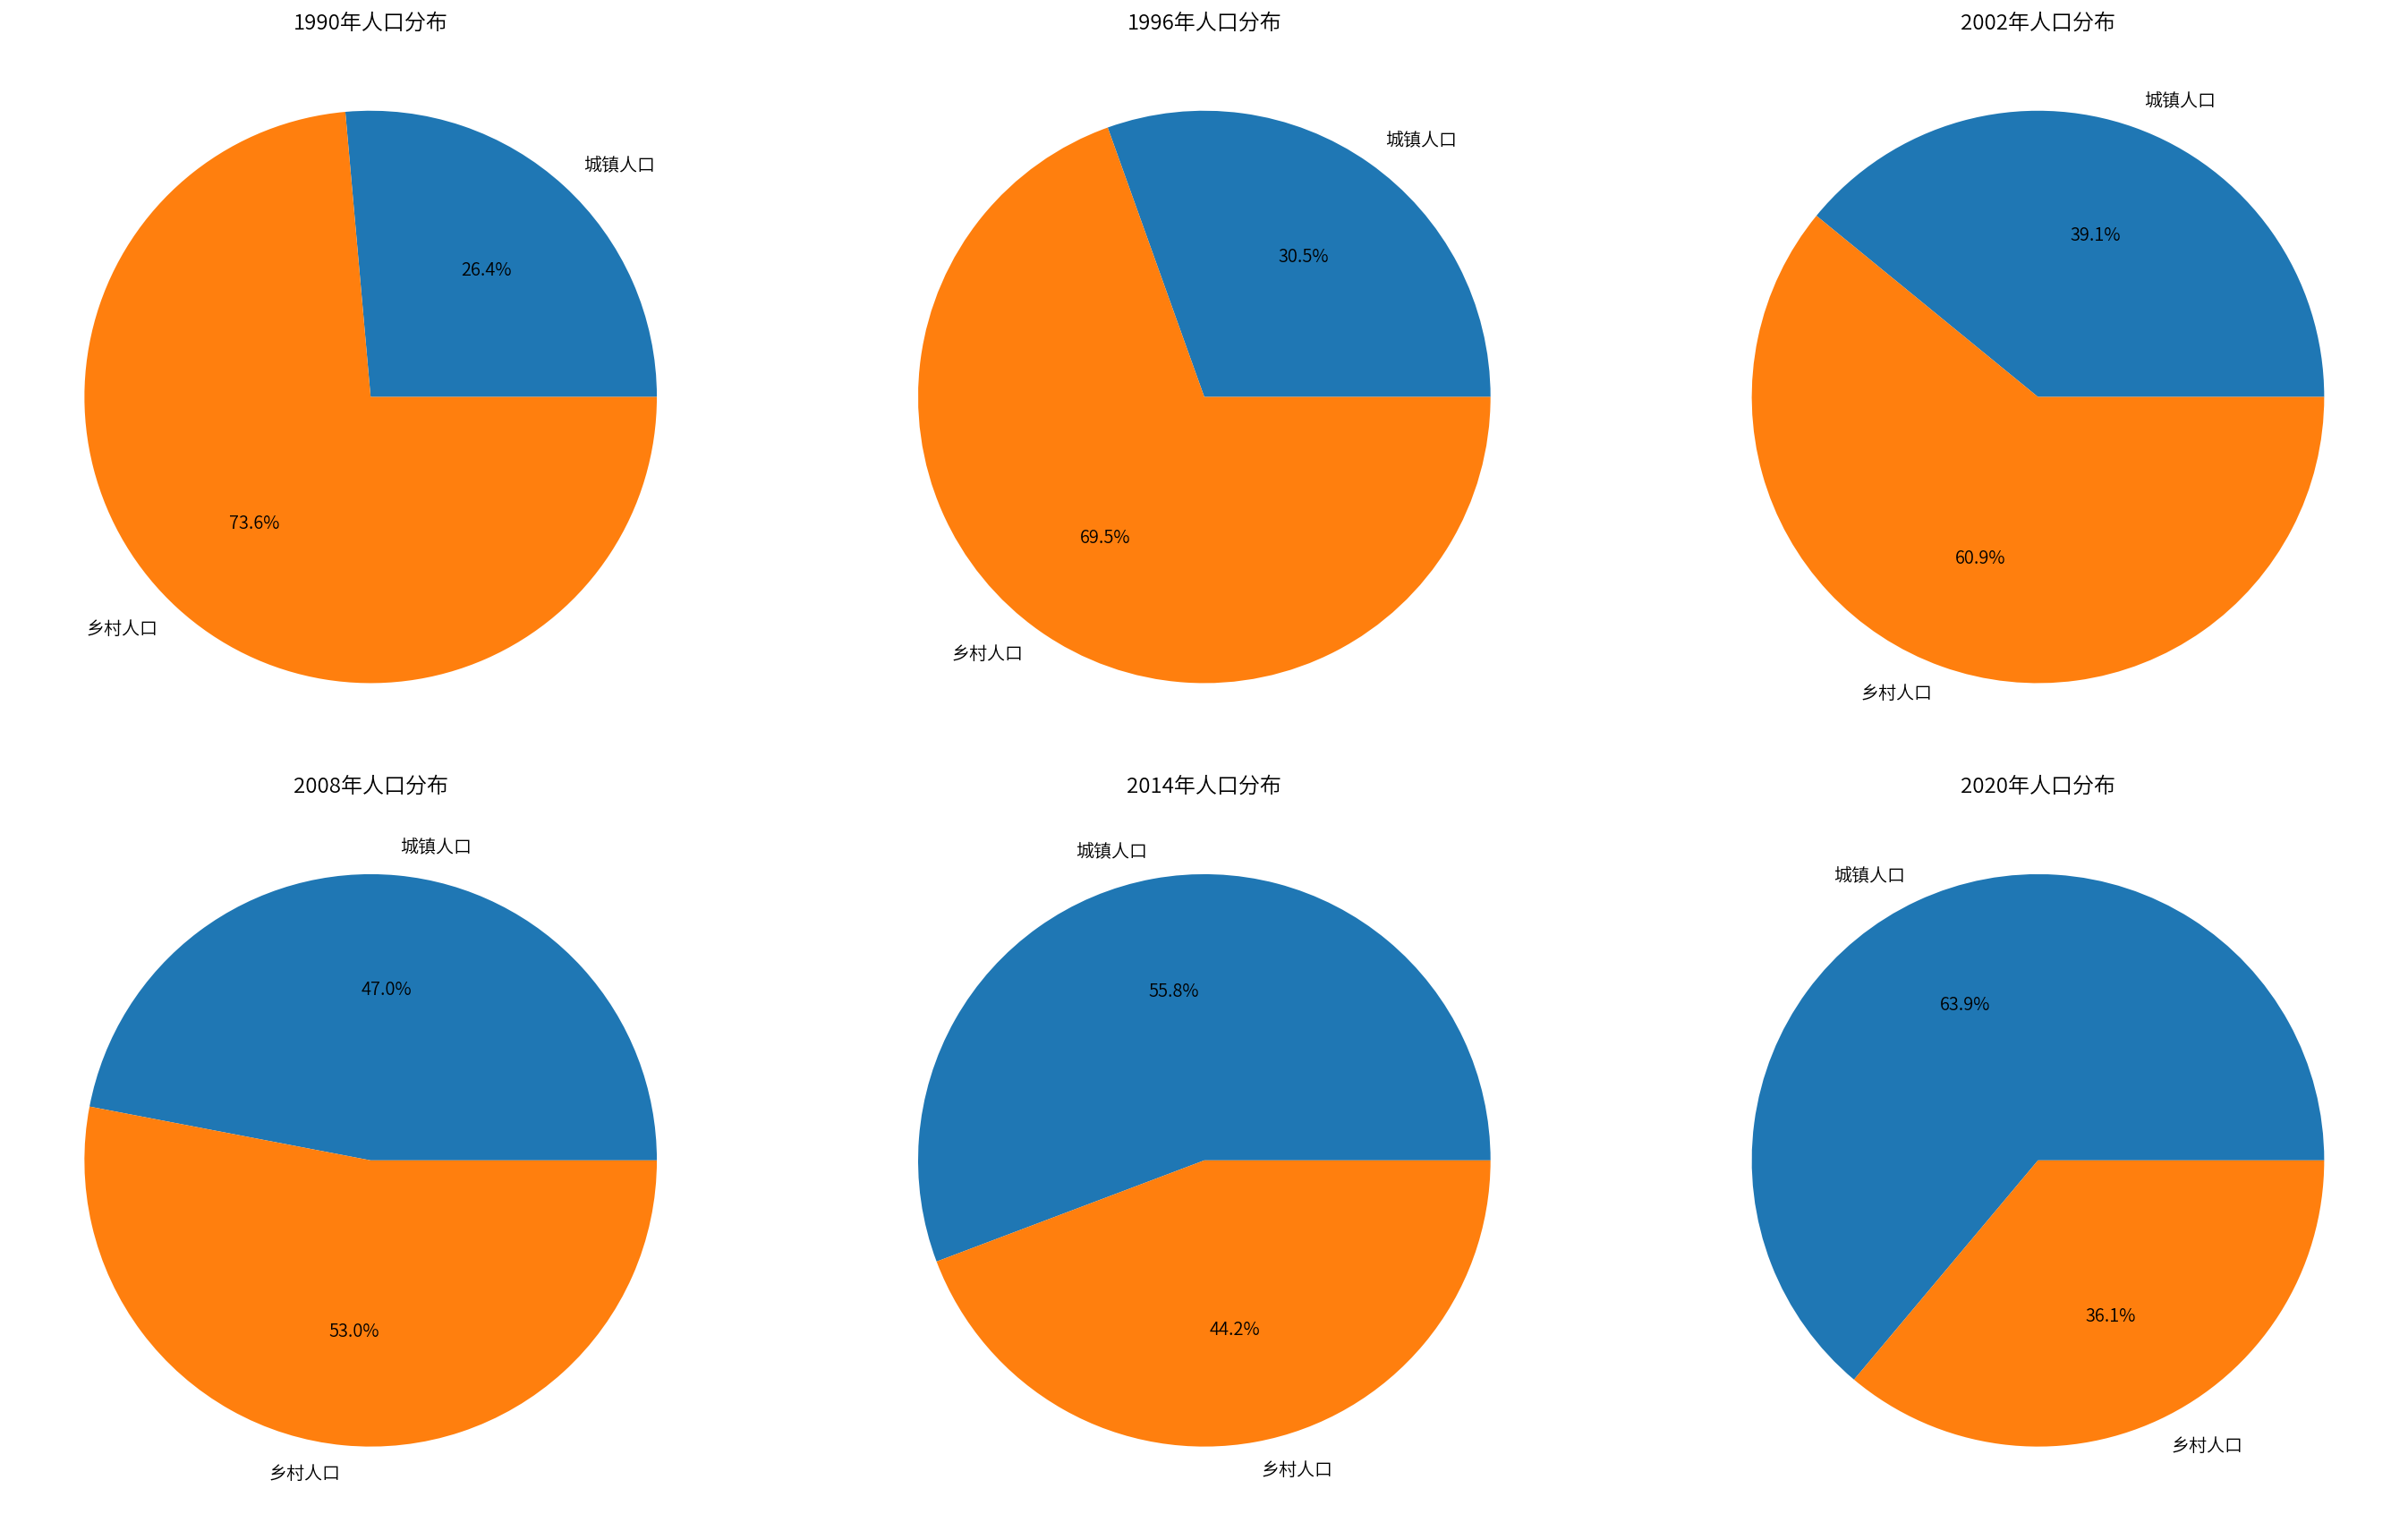
\includegraphics[width=1\linewidth]{figures/1.png}
    \caption{�����˿�ռ��ͼ}
    \label{fig:city_village_population}
\end{figure}

ͼ����ʾ�������˿�ռ������������������˿�ռ����Ӧ�������½�����һ������ĸ↑�������й����л����̵ļӿ�������ء�

% �����й����õĿ��ٷ�չ����ҵ����������Լ��������������ij������ƣ�����ũ�����������������Ѱ����õĹ�����������ᡣ��һ���Ƶ��³����˿ڱ�������������������˿ڱ�����Ӧ�������½��������˿�����������ӳ�˳���֮��ľ��ò�࣬Ҳ��ʾ��ũ������ڷ�չ���ᡢ������ʩ��������ҽ�Ƶȷ���IJ��㡣

ũ��������˿���ʧ��һ��͹����ũ�巢չ����������Ϊ�˻�����һ���ƣ������ǿũ�彨��������������ṩ����ľ�ҵ���ᣬ���ƽ�����ҽ���������Լ����ũ�������ˮƽ��Ϊũ����������������������͹�����������������˿ڵ���ʧ�ٶȣ��ٽ�����Э����չ����������������ʷ�����£��������ս��Ӧ�˶�������Ϊ���й���ɫ���������ʱ������Ҫƪ�¡�

\section{�����˿�Ԥ��}
��һ���������֣���������˿ڱ��������½������½����ٶ��ƺ��ڷŻ�����ʾ���������ٵķ����𽥼�С������ܷ�ӳ�˽������й����ƽ����緢չһ�廯��ʵʩ�������ս�Եȷ���������Ŭ����ʼ���ֳ�Ч������˿���ʧ�ٶ������Ż���

Ϊ����֤�����˿ڱ仯���ƵIJ��벢Ԥ��δ����չ�����IJ�����DLF-LSTMģ��Ԥ������������ڳ����˿ڵı仯���ơ����õ���Ԥ�����Լ�ģ�Ͷ���ʷ���ݵ�������ͨ����ͼչʾ��
\begin{figure}[H]
    \centering
    \begin{minipage}{0.5\textwidth}
        \centering
        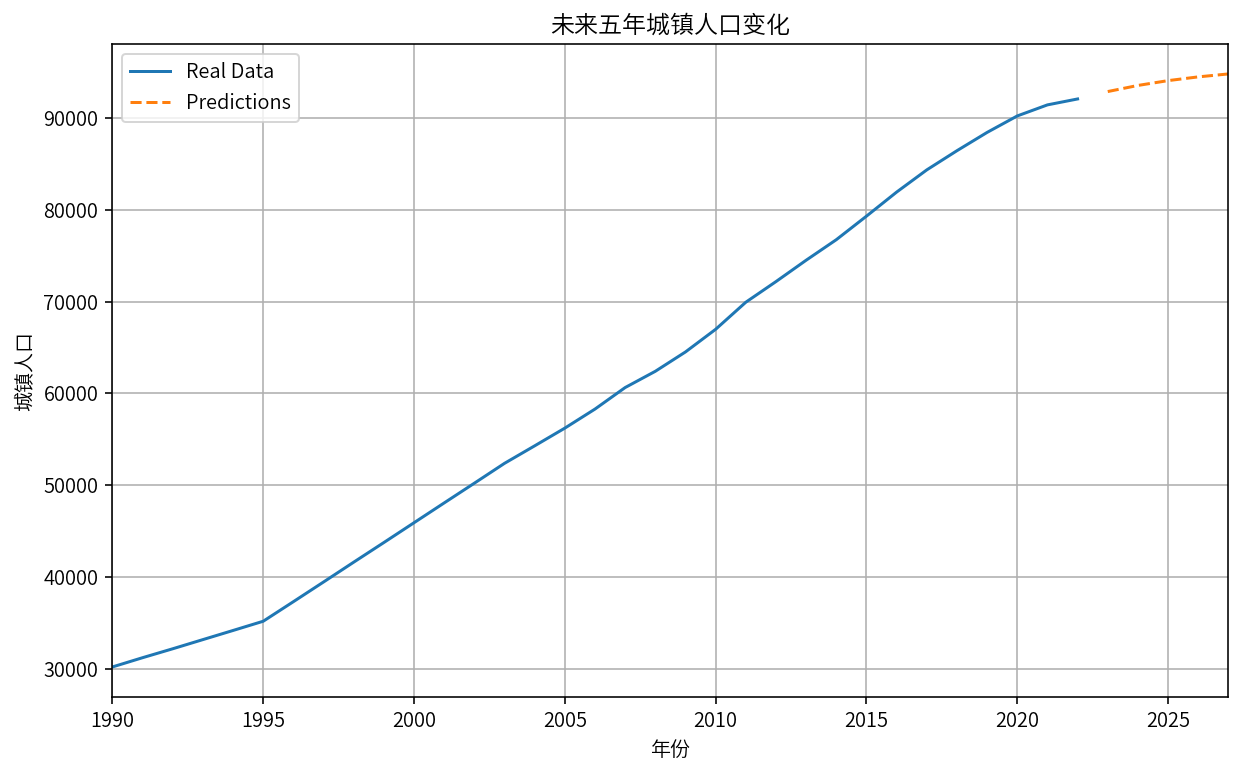
\includegraphics[width=\linewidth]{figures/2.png}
        \caption{δ����������˿ڱ仯}
        \label{fig:population-change}
    \end{minipage}\hfill
    \begin{minipage}{0.5\textwidth}
        \centering
        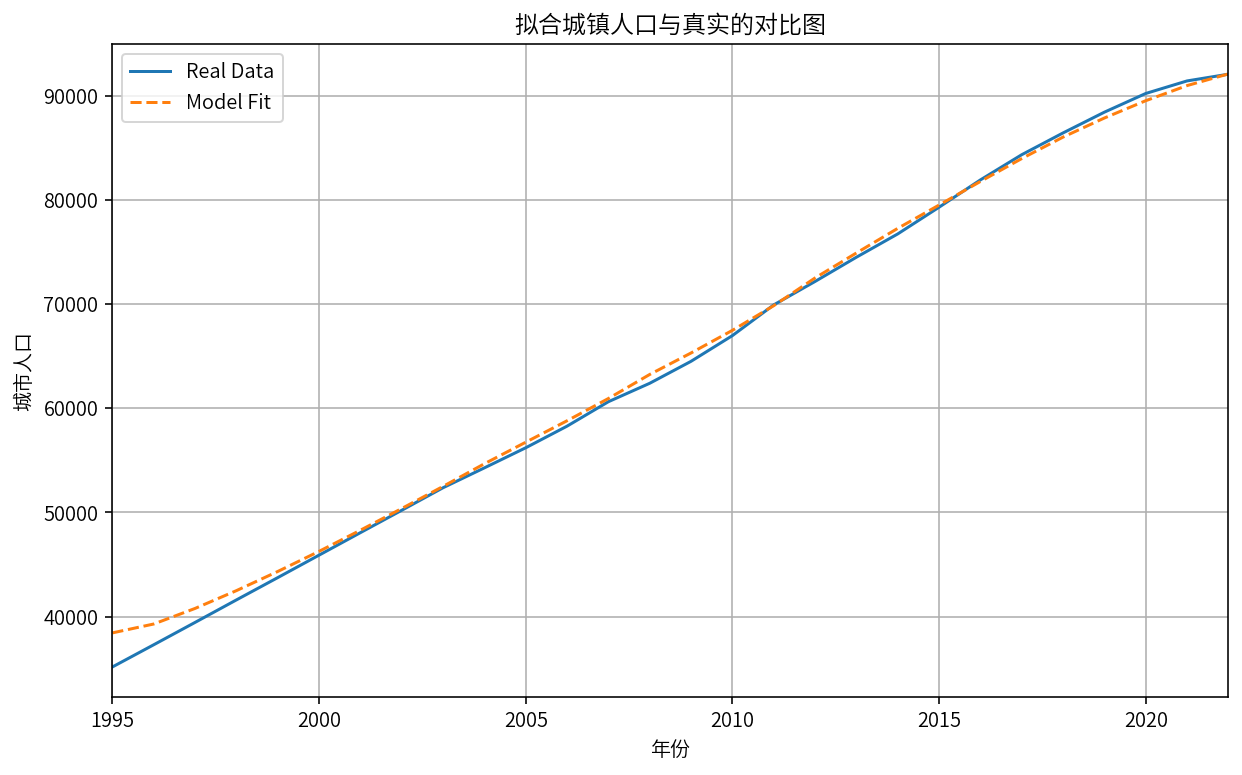
\includegraphics[width=\linewidth]{figures/3.png}
        \caption{��ϳ����˿ں���ʵ�ĶԱ�ͼ}
        \label{fig:population_fit-vs-real}
    \end{minipage}
\end{figure}

ͨ��ʱ�����е�֪�������������ƿ��ܳ��ֱ��ͣ�ֻ����΢��������

����ͬ����������ũ���˿ڵ�Ԥ�⣬���ý�����£�
\begin{figure}[H]
    \centering
    \begin{subfigure}{0.5\textwidth}
        \centering
        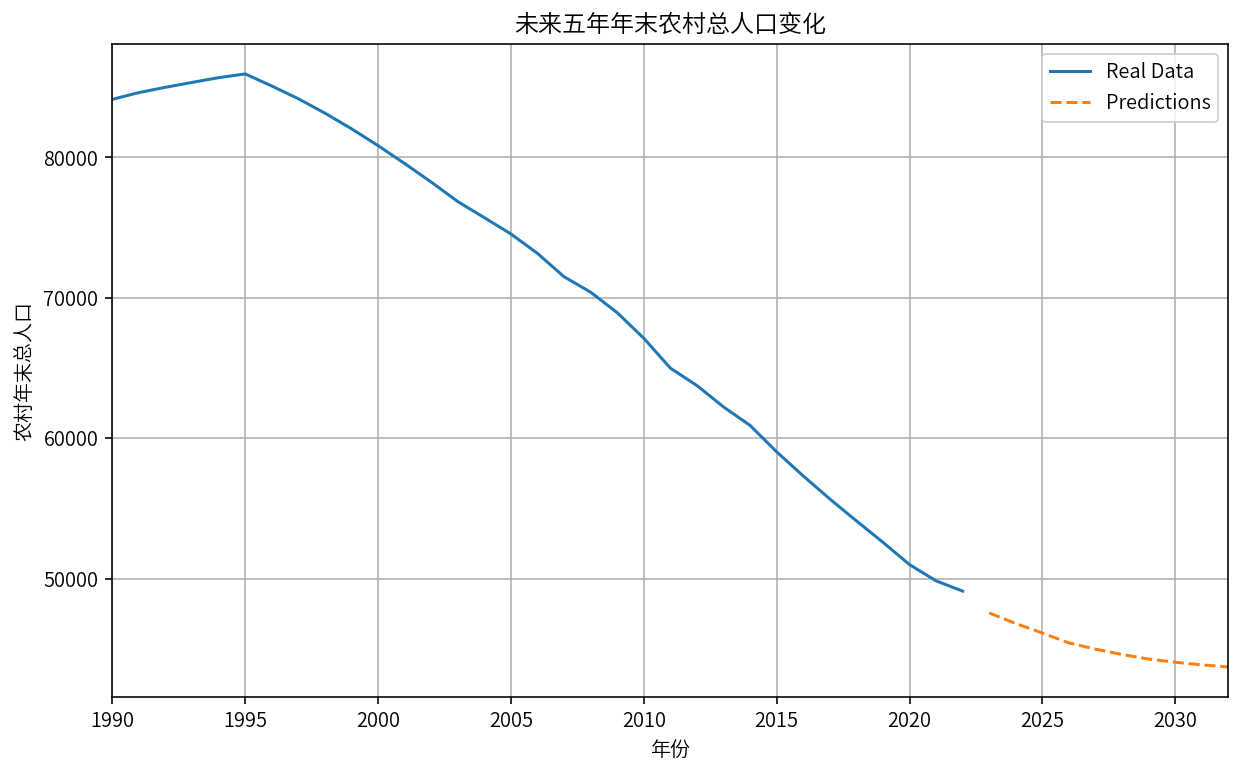
\includegraphics[width=\linewidth]{figures/35.png}
        \caption{δ������ũ���˿ڱ仯}
        \label{fig:sub1}
    \end{subfigure}%
    \begin{subfigure}{0.5\textwidth}
        \centering
        \includegraphics[width=\linewidth]{figures/36.png}
        \caption{���ũ���˿ں���ʵ�ĶԱ�ͼ}
        \label{fig:sub2}
    \end{subfigure}
    \caption{ũ���˿ڱ仯ͼ}
    \label{fig:combined}
\end{figure}

\begin{table}[h]
    \centering
    \begin{minipage}{0.48\linewidth}
        \centering
        \caption{δ�������˿�Ԥ��}
        \label{tab:urban_population_prediction}
        \begin{tabular}{cc}
        \hline
        ��� & Ԥ������˿�(����) \\
        \hline
        2023 & 92876.58 \\
        2024 & 93542.80 \\
        2025 & 94068.30 \\
        2026 & 94475.73 \\
        \hline
        \end{tabular}
    \end{minipage}\hfill
    \begin{minipage}{0.48\linewidth}
        \centering
        \caption{δ��ũ�����˿�Ԥ��}
        \label{tab:rural_population_prediction}
        \begin{tabular}{cc}
        \hline
        ��� & Ԥ��ũ�����˿�(����) \\
        \hline
        2023 & 47548.48 \\
        2024 & 46795.32 \\
        2025 & 46118.73 \\
        2026 & 45412.10 \\
        \hline
        \end{tabular}
    \end{minipage}
\end{table}



��󣬱��Ķ�ÿ��ũ���˿ڱ仯��ǰһ��ı��������˻��ܣ����Ƚ�������1�Ĵ�С������������ӽ�1ʱ��˵��ũ���˿ڵļ���������Խ�С�������������Զ��1ʱ������ζ�ű仯���Ƚϴ�

\begin{figure}[H]
    \centering
    \includegraphics[width=0.65\linewidth]{figures/37.png}
    \caption{���ũ�����˿��½�����}
    \label{fig:enter-label}
\end{figure}
���ߵĽ������ʾ��ũ���˿�δ���ı仯���ƻ������ܵ�����������ߵĻ���Ӱ�죬���ֳ�������ƽ�����������������ӵ�̬�ơ��ⰵʾ����δ��һ��ʱ���ڣ�ũ��������ܻ�ӭ��һ���̶ȵ��˿ڻ�������������������ս���������Ļ��������

��һս�Բ����Ƕ��й�ũ���������̷�˼�����Ƕ�ʵ�ֳ����г��չԸ���ļᶨ׷���ڴ�ս���£�ũҵ�����ǵ�һ����ʳ����������ת��Ϊ�ִ�������Ԫ���IJ�ҵ��ϵ��ũ�岻�������Ĵ����ʣ����dz�Ϊ����������ϣ�������ء�ũ������ʱ���ı�Ե�ˣ����dz�Ϊ�����ִ������ɹ������塣

% һ���棬һЩ����ͨ������ũ������������ũҵ��ҵ�����������ɹ����������˿ڷ��紴ҵ��ع�ũҵ�����γ��˳����˿�������˫�򻥶�ģʽ����һ���棬����ũ�������ҽ�ƺ����������ĸ��ƣ�ũ����������������������ũ��������˿�����ѹ���������⣬���������ʼ���ֳ����ӻ����Ϳɳ�����չ��̬�ơ���Щ�仯��ӳ���������ս���ڵ����˿ڽṹ���ٽ�������ⷢչ����Ļ�����Ч��


\chapter{结论和展望}
\label{chapter:conclusion}
\begin{tikzpicture}[remember picture,overlay]
\node[inner sep=0pt,opacity=0.3] at (current page.center) { % Adjust the opacity here
    \includegraphics[width=\paperwidth,height=\paperheight]{figures/OIP-C.jpg} % Replace 'background.jpg' with your image file
};
\end{tikzpicture}

在当前的发展阶段,乡村振兴不仅关乎农业、农村和农民的未来,更是国家战略全局的重要组成部分。通过本次数据分析报告,我们得出了一写结论和展望。

必须继续大力稳固粮食安全,这是国家的根本。正如习主席所强调的,“要把中国人的饭碗牢牢端在自己手中”,我们将继续保持粮食生产的稳定性,确保每一粒粮食都能得到妥善利用。

数字农业的发展是提升农业现代化水平的关键。尽管当前数字农业渗透率尚显不足,但我们将加强数字技术在农业中的应用,推动农业生产方式的转变,如《2020年中国农村数字发展报告》所述,通过数字化转型,实现农业的智能化、精准化。

对于偏远地区,推进基础设施建设是实现乡村振兴的前提。我们将加大投资力度,改善交通、水利、电力等基础设施,为乡村发展提供坚实的物质基础。

乡村旅游业的发展是乡村振兴的一大亮点。我们将依托各地的自然风光和文化遗产,打造特色旅游产品,吸引更多游客,带动乡村经济的多元化发展。

优化产业结构,促进私营企业和个体户的发展,是提高农村经济效益的重要途径。我们将制定更多优惠政策,支持乡村产业的创新和升级,增强乡村经济的内生动力。

为促进人口回流,我们将继续完善公共服务,提高农村居民的生活质量,使乡村成为人们向往的美好家园。如习主席所言,“要让农民在乡村振兴中有更多获得感”,我们将努力实现城乡居民的共同富裕。

乡村振兴战略的实施,需要我们在保障粮食安全、推进数字农业、加强基础设施建设、发展乡村旅游业、优化产业结构和促进人口回流等多个方面下功夫。我们将以实事求是的态度,贯彻落实两会精神和三农政策,为实现乡村全面振兴而不懈努力!





\setcounter{biburlnumpenalty}{7000}
\setcounter{biburllcpenalty}{7000}
\setcounter{biburlucpenalty}{7000}
\printbibliography[heading=bibintoc,title=参考文献]

%\newpage
\section{Appendix}
\begin{lstlisting}[language=python,caption={两会数据爬虫}]
# 两会是现在的热门话题,从两会讨论的话题中,来看乡村发展的必要性
import requests
from bs4 import BeautifulSoup
headers = {
    "User-Agent": "Mozilla/5.0 (Windows NT 10.0; Win64; x64) AppleWebKit/537.36 (KHTML, like Gecko) Chrome/121.0.0.0 Safari/537.36 Edg/121.0.0.0"
}
texts = [] # 提取两会文本
for i in range(0,9):
    if(i!=0) :
        url = f"https://www.gov.cn/zhuanti/2024qglh/2024nzfgzbg/home_{i}.htm"
    else:
        url = "https://www.gov.cn/zhuanti/2024qglh/2024nzfgzbg/home.htm"
    response = requests.get(url,headers=headers)
    response.encoding="utf-8"
    content = response.text
    soup = BeautifulSoup(content,"html.parser")
    # 定位到特定的<div>容器
    container = soup.find('div', class_="list list_1 list_2")
    # 在这个容器内查找所有的<a>标签
    links = container.find_all('a')
    # 提取并打印所有<a>标签的文本内容
    for link in links:
        texts.append(link.get_text())
print(texts)
# 筛选出包含 '乡' 字的文本项
texts_containing_char = [text for text in texts if '农' in text or '乡' in text  or '村' in text or '城' in text or '绿' in text]

# 打印结果
for text in texts_containing_char:
    print(text)
    ## 输出高清图像
%config InlineBackend.figure_format = 'retina'
%matplotlib inline
import numpy as np
import matplotlib.pyplot as plt
from wordcloud import WordCloud
 
text = "Love"
 
x, y = np.ogrid[:300, :300]
 
mask = (x - 150) ** 2 + (y - 150) ** 2 > 130 ** 2
mask = 255 * mask.astype(int)
wc = WordCloud(background_color="white", repeat=True, mask=mask)
wc.generate(text)
 
plt.axis("off")
plt.imshow(wc, interpolation="bilinear")
plt.show()
import numpy as np
import matplotlib.pyplot as plt
from wordcloud import WordCloud
 
# 合并文本数据
text = """
从两会看中国经济:打好乡村全面振兴漂亮仗
推动城乡融合和区域协调发展 大力优化经济布局
扎实推进乡村全面振兴
推动城乡融合和区域协调发展
推动传统产业高端化、智能化、绿色化转型!
政府工作报告中的绿色低碳发展
今年要把促进农业转移人口市民化放在突出位置来抓
加强生态文明建设,推进绿色低碳发展
推动城乡融合和区域协调发展,大力优化经济布局
坚持不懈抓好“三农”工作,扎实推进乡村全面振兴
"""
 
x, y = np.ogrid[:300, :300]
 
mask = (x - 150) ** 2 + (y - 150) ** 2 > 130 ** 2
mask = 255 * mask.astype(int)
 
 
wc = WordCloud(background_color="white", repeat=True, mask=mask)
wc.generate(text)
 
plt.axis("off")
plt.imshow(wc, interpolation="bilinear")
plt.show()
from wordcloud import WordCloud
import matplotlib.pyplot as plt

# Your text data
text = """
从两会看中国经济:打好乡村全面振兴漂亮仗
推动城乡融合和区域协调发展 大力优化经济布局
扎实推进乡村全面振兴
推动城乡融合和区域协调发展
推动传统产业高端化、智能化、绿色化转型!
政府工作报告中的绿色低碳发展
今年要把促进农业转移人口市民化放在突出位置来抓
加强生态文明建设,推进绿色低碳发展
推动城乡融合和区域协调发展,大力优化经济布局
坚持不懈抓好“三农”工作,扎实推进乡村全面振兴
"""

# Generating the word cloud
wordcloud = WordCloud(
    font_path='/home/mw/project/SourceHanSansSC-Regular.ttf',
    background_color='white',
    collocations=False,
    max_words=50,
    max_font_size=100,
    min_font_size=10,
    scale=10
).generate(text)

# Displaying the word cloud image
plt.figure(figsize=(10, 5))
plt.imshow(wordcloud, interpolation='bilinear')
plt.axis('off')
plt.show()
from wordcloud import WordCloud
import matplotlib.pyplot as plt

# 合并文本数据
text = """
从两会看中国经济:打好乡村全面振兴漂亮仗
推动城乡融合和区域协调发展 大力优化经济布局
扎实推进乡村全面振兴
推动城乡融合和区域协调发展
今年要把促进农业转移人口市民化放在突出位置来抓
推动城乡融合和区域协调发展,大力优化经济布局
坚持不懈抓好“三农”工作,扎实推进乡村全面振兴
"""

# 生成词云,增加scale参数
wordcloud = WordCloud(
    font_path='/home/mw/project/SourceHanSansSC-Regular.ttf',
    width=800,
    height=400,
    background_color='white',
    collocations=False,
    max_words=50,
    max_font_size=100,
    min_font_size=10,
    scale=2  # 增加输出图像的分辨率
).generate(text)

# 显示词云图像
plt.figure(figsize=(10, 5))
plt.imshow(wordcloud, interpolation='bilinear')
plt.axis('off')
plt.show()
import jieba.posseg as pseg
\end{lstlisting}
\begin{lstlisting}[language=python,caption={全国乡村产业发展规划}]
file_path = '/home/mw/input/planning5088/《全国乡村产业发展规划(2020-2025年)》全文.txt'

with open(file_path, 'r', encoding='utf-8') as file:
    article_content = file.read()
    ## 输出高清图像
%config InlineBackend.figure_format = 'retina'
%matplotlib inline
import re
cleaned_content = re.sub(r'[^\w\s]', '', article_content) 
cleaned_content = re.sub(r'\d', '', cleaned_content)     
cleaned_content = cleaned_content.replace('\n', '')
import jieba as jb
from wordcloud import WordCloud
import matplotlib.pyplot as plt
words_to_remove = ['乡村', '农村', '农业', '产业', '发展', '振兴','的','等','和']
for word in words_to_remove:
    cleaned_content = cleaned_content.replace(word, '')
    cleaned_content = jb.lcut(cleaned_content)
cleaned_content  =  '/'.join(cleaned_content)
wordcloud = WordCloud(collocations=False,font_path='/home/mw/project/SourceHanSansSC-Regular.ttf', width=3000, height=2000, margin=2,background_color='white').generate(cleaned_content)
# 显示图片 
plt.imshow(wordcloud) 
plt.axis('off')
plt.show()

\end{lstlisting}
\begin{lstlisting}[language=python,caption={主要农作物播种面积和产品产量数据
}]
import pandas as pd
file_path = '/home/mw/input/develop6699/主要农作物播种面积和产品产量数据.csv'
data = pd.read_csv(file_path,encoding='GBK')
# 按照时间为列做整理
data = data.set_index('指标').T
data.reset_index(inplace=True)
data.rename(columns={'index': '年份'}, inplace=True)
data.head()
# 改为数值方便统计
data['年份'] = data['年份'].str.replace('年', '')
data = data.sort_values(by='年份')
data.head()
## 输出高清图像
%config InlineBackend.figure_format = 'retina'
%matplotlib inline
import seaborn as sns
import matplotlib.pyplot as plt
selected_columns = ['年份', '小麦产量(万吨)', '稻谷产量(万吨)', '大豆产量(万吨)', '玉米产量(万吨)']
heatmap_data = data[selected_columns].set_index('年份')
heatmap_data = heatmap_data.astype('float').transpose()
step = len(filtered_heatmap_data.columns) // 5  
years_to_display = filtered_heatmap_data.columns[::step]
plt.figure(figsize=(10, 6))
for crop in filtered_heatmap_data.index:
    plt.plot(filtered_heatmap_data.columns, filtered_heatmap_data.loc[crop], marker='o', label=crop)

plt.xticks(years_to_display, [int(year) for year in years_to_display])

plt.title('主要粮食产量变化')
plt.xlabel('年份')
plt.ylabel('产量')
plt.legend()
plt.grid(True)
plt.show()
# 输出每种农作物随时间的变化
# 每条折线为不同类型农作物的播种面积
import matplotlib.pyplot as plt

indicators = data.columns[1:] 
indicator_groups = [indicators[i:i + 10] for i in range(0, len(indicators), 10)]
for i, group in enumerate(indicator_groups):
    plt.figure(figsize=(15, 8))
    for indicator in group:
        plt.plot(data['年份'], data[indicator], label=indicator)

    plt.title(f'农作物播种面积和产量指标:图 {i+1}')
    plt.xlabel('年份')
    plt.ylabel('数值')
    plt.xticks(rotation=45)
    plt.legend()
    plt.grid(True)
    plt.tight_layout()
    plt.show()
    import matplotlib.pyplot as plt


selected_indicators = transposed_data.columns[1:10] 

plt.figure(figsize=(15, 8))

for year in transposed_data['年份']:
    plt.plot(selected_indicators, transposed_data[transposed_data['年份'] == year].iloc[0, 1:10], label=year)

plt.xlabel('指标')
plt.ylabel('面积/产量')
plt.title('1990-2022年各指标的年度变化')
plt.xticks(rotation=45)
plt.legend(loc='upper left', ncol=2, title='年份')
plt.grid(True)
plt.show()

# 输出每种农作物随时间的变化
# 每条折线为时间线

import matplotlib.pyplot as plt


indicator_groups = [data.columns[1:][i:i + 10] for i in range(0, len(data.columns[1:]), 10)]


for i, group in enumerate(indicator_groups):
    plt.figure(figsize=(15, 8))


    for year in data['年份']:
        plt.plot(group, data[data['年份'] == year].iloc[0][group], label=year)

    plt.xlabel('指标')
    plt.ylabel('面积/产量')
    plt.title(f'1990-2022年各指标的年度变化 - 图 {i+1}')
    plt.xticks(rotation=45, ha='right')
    plt.legend(loc='upper left', ncol=2, title='年份')
    plt.grid(True)
    plt.tight_layout()
    plt.show()
    import numpy as np

# 准备玫瑰图的数据
categories = data['年份']
values = data['农作物总播种面积(千公顷)']
N = len(categories)

# 计算每个类别的角度
angles = [n / float(N) * 2 * np.pi for n in range(N)]
values = np.concatenate((values, [values[0]]))  # 闭合图形
angles += angles[:1]

# 计算平均值以标准化数据
mean_value = data['农作物总播种面积(千公顷)'].mean()

# 标准化值(与平均值的差异)
normalized_values = data['农作物总播种面积(千公顷)'] - mean_value

plt.figure(figsize=(12, 8))
ax = plt.subplot(111, polar=True)

# 绘制标准化的值
ax.plot(angles, list(normalized_values) + [normalized_values[0]])
ax.fill(angles, list(normalized_values) + [normalized_values[0]], 'b', alpha=0.1)

plt.xticks(angles[:-1], categories, color='black', size=10)
plt.title('1990-2022年农作物总播种面积的变化(相对于平均值) - 玫瑰图')
plt.show()


\end{lstlisting}\begin{lstlisting}[language=python,caption={十四五规划可视化}]
import pandas as pd
# 读取数据时使用GBK
file_path = '/home/mw/input/1458039/十四五计划.csv'
data = pd.read_csv(file_path,encoding='GBK')
data.head()
## 输出高清图像
%config InlineBackend.figure_format = 'retina'
%matplotlib inline
import pandas as pd
import matplotlib.pyplot as plt
# 为了排版美观,将数据进行翻转
# 转置数据框,使得各个指标成为行,年份成为列
data_transposed = data.set_index('年份').T
data_transposed.columns = data_transposed.columns.map(str)  # 将年份的列名转换为字符串

# 对每个指标的数据进行归一化处理,确保其和为1(或100%)
data_normalized = data_transposed.div(data_transposed.sum(axis=1), axis=0)

# 绘制堆叠条形图,纵坐标为各种指标,每个条形图内部展示2020年和2025年数据的百分比
ax = data_normalized.plot(kind='barh', stacked=True, figsize=(10, 8))

# 设置图例
ax.legend(title='年份', loc='center left', bbox_to_anchor=(1, 0.5))

# 添加标签和标题
ax.set_xlabel('百分比')
ax.set_ylabel('指标')
ax.set_title('各指标在2020年与2025年的百分比堆叠条形图')

# 显示图表
plt.tight_layout()
plt.show()
\end{lstlisting}
\begin{lstlisting}[language=python,caption={主要贡献}]
import pandas as pd
file_path = '/home/mw/input/develop6699/全国农业主要科技贡献相关指标.csv'
data = pd.read_csv(file_path)
print(data)
## 图像显示中文的问题
import matplotlib

import seaborn as sns

## 输出高清图像
%config InlineBackend.figure_format = 'retina'
%matplotlib inline
import matplotlib.pyplot as plt
# Creating the time series plot without using sns.set
plt.figure(figsize=(15, 8))
sns.lineplot(x='时间', y='数值', hue='品类', data=filtered_data, marker='o')

# Adding title and labels
plt.title('全国农业主要科技贡献相关指标的时间序列图')
plt.xlabel('年份')
plt.ylabel('数值 (%)')
plt.xticks(rotation=45)
# plt.legend(title='品类')

# Show the plot
plt.show()
import numpy as np

# Preparing data for the heatmap
# Pivot the data to get years as columns and categories as rows
heatmap_data = data.pivot_table(values='数值', index='品类', columns='时间', aggfunc=np.mean)

# Creating the heatmap
plt.figure(figsize=(12, 8))
sns.heatmap(heatmap_data, annot=True, cmap='YlGnBu', linewidths=.5)

# Adding title and labels
plt.title('全国农业主要科技贡献相关指标的热力图')
plt.xlabel('年份')
plt.ylabel('品类')

# Show the plot
plt.show()
\end{lstlisting}
\begin{lstlisting}[language=python,caption={数字农业渗透}]
## 输出高清图像
%config InlineBackend.figure_format = 'retina'
%matplotlib inline
import pandas as pd

# 读取数据时使用GBK
file_path = '/home/mw/input/shentou8131/数字农业渗透率.csv'
data = pd.read_csv(file_path,encoding='GBK')

print(data)
## 输出高清图像
%config InlineBackend.figure_format = 'retina'
%matplotlib inline
import matplotlib.pyplot as plt
import numpy as np
# 将百分数改为浮点数值
data['渗透率'] = data['年份'].str.rstrip('%').astype('float')

# 计算同比变化率
data['变化率'] = data['渗透率'].pct_change() * 100

# 计算每年的渗透率差异
data['年度差值'] = data['渗透率'].diff()

# 创建一个包含渗透率的条形图
fig, ax1 = plt.subplots()

color = 'tab:blue'
ax1.set_xlabel('年份')
ax1.set_ylabel('数字化渗透率 (%)', color=color)
ax1.bar(data['农业数字化渗透率'], data['渗透率'], color=color, alpha=0.6)
ax1.tick_params(axis='y', labelcolor=color)

# 创建带有年度差异的折线图
ax2 = ax1.twinx()  
color = 'tab:red'
ax2.set_ylabel('年度差值 (%)', color=color)  
ax2.plot(data['农业数字化渗透率'], data['年度差值'], color=color, marker='o', linestyle='-', linewidth=2)
ax2.tick_params(axis='y', labelcolor=color)

fig.tight_layout()  
plt.title('农业数字化渗透率及其年度差值')
plt.show()
# 更正列标头及其值
data.columns = ['年份', '农业数字化渗透率']
data['农业数字化渗透率'] = data['农业数字化渗透率'].str.rstrip('%').astype(float) / 100
data
import torch
import torch.nn as nn
import numpy as np
import matplotlib.pyplot as plt
from sklearn.preprocessing import MinMaxScaler
## 封装成一个函数,便于调用(用于处理字典)

def predict(data, train_window, future_pred, label, epochs,lr):

    # 转换为 numpy 数组
    data_np = np.array(data[label]).reshape(-1, 1)

    # 数据归一化
    scaler = MinMaxScaler(feature_range=(-1, 1))
    data_normalized = scaler.fit_transform(data_np)

    # 转换为 PyTorch tensors
    data_normalized = torch.FloatTensor(data_normalized).view(-1)

    # 创建数据集
    def create_inout_sequences(input_data, tw):
        inout_seq = []
        L = len(input_data)
        for i in range(L-tw):
            train_seq = input_data[i:i+tw]
            train_label = input_data[i+tw:i+tw+1]
            inout_seq.append((train_seq, train_label))
        return inout_seq

    train_inout_seq = create_inout_sequences(data_normalized, train_window)

    # 定义 LSTM 模型
    class LSTM(nn.Module):
        def __init__(self, input_size=1, hidden_layer_size=100, output_size=1):
            super().__init__()
            self.hidden_layer_size = hidden_layer_size

            self.lstm = nn.LSTM(input_size, hidden_layer_size)

            self.linear = nn.Linear(hidden_layer_size, output_size)

            self.hidden_cell = (torch.zeros(1, 1, self.hidden_layer_size),
                                torch.zeros(1, 1, self.hidden_layer_size))

        def forward(self, input_seq):
            lstm_out, self.hidden_cell = self.lstm(input_seq.view(len(input_seq), 1, -1), self.hidden_cell)
            predictions = self.linear(lstm_out.view(len(input_seq), -1))
            return predictions[-1]

    # 实例化模型
    model = LSTM()
    loss_function = nn.MSELoss()
    optimizer = torch.optim.Adam(model.parameters(), lr)

    # 训练模型
    # epochs = 25

    loss_values = [] 

    for epoch in range(epochs):
        for seq, labels in train_inout_seq:
            optimizer.zero_grad()
            model.hidden_cell = (torch.zeros(1, 1, model.hidden_layer_size),
                                torch.zeros(1, 1, model.hidden_layer_size))

            y_pred = model(seq)

            single_loss = loss_function(y_pred, labels)
            single_loss.backward()
            optimizer.step()

        if epoch % 5 == 1:
            loss_values.append(single_loss.item())  # Store the loss value
            print(f'epoch: {epoch:3} loss: {single_loss.item():10.8f}')

    print(f'epoch: {epoch:3} loss: {single_loss.item():10.10f}')





    # 使用matplotlib绘制图形
    plt.figure(figsize=(10, 6))
    plt.plot(loss_values, marker='o', linestyle='-', color='b')
    plt.title('Loss Reduction Over Epochs')
    plt.xlabel('Epoch')
    plt.ylabel('Loss')
    plt.grid(True)
    plt.show()


    # 使用模型对整个数据集进行预测以创建拟合与真实数据对比图
    # 为预测做准备
    test_inputs = data_normalized[-train_window:].tolist()

    # 预测未来
    model.eval()
    for i in range(future_pred):
        seq = torch.FloatTensor(test_inputs[-train_window:])
        with torch.no_grad():
            model.hidden_cell = (torch.zeros(1, 1, model.hidden_layer_size),
                                torch.zeros(1, 1, model.hidden_layer_size))
            test_inputs.append(model(seq).item())
    # 将预测数据转换回原始规模
    actual_predictions = scaler.inverse_transform(np.array(test_inputs[train_window:]).reshape(-1, 1))
    predicted_years = np.arange(data["年份"].iloc[-1] + 1 - train_window, data["年份"].iloc[-1] + 1 + future_pred)


    # # 输出预测的未来私营企业乡村就业人员数值
    # predicted_years = np.arange(data["年份"][-1] + 1 - train_window, data["年份"][-1] + 1 + future_pred)
    for year, population in zip(predicted_years, actual_predictions):
        print(f"年份: {year}, 预测{label}(万人): {population[0]:.2f}")

    # 绘制图表
    plt.figure(figsize=(10, 6))
    plt.title(f'未来{label}变化预测')
    plt.xlabel('年份')
    plt.ylabel(f'{label}')
    plt.grid(True)
    plt.autoscale(axis='x', tight=True)
    
    # 绘制实际数据
    plt.plot(data["年份"], data[label], label='Real Data')
    
    # 绘制预测数据
    plt.plot(predicted_years, np.concatenate([data[label][-train_window:], actual_predictions.ravel()]), label='Predictions', linestyle='--')
    
    plt.legend()
    plt.show()
    # # 将预测数据转换回原始规模
    # actual_predictions = scaler.inverse_transform(np.array(test_inputs[train_window:]).reshape(-1, 1))

    # # 输出预测的未来私营企业乡村就业人员数值
    # predicted_years = np.arange(data["年份"][-1] + 1, data["年份"][-1] + 1 + future_pred)
    # for year, population in zip(predicted_years, actual_predictions):
    #     print(f"年份: {year}, 预测{label}(万人): {population[0]:.2f}")

    # # 绘制图表
    # plt.figure(figsize=(10, 6))
    # plt.title(f'未来{label}变化预测')
    # plt.xlabel('年份')
    # plt.ylabel(f'{label}')
    # plt.grid(True)
    # plt.autoscale(axis='x', tight=True)
    # plt.plot(data["年份"], data[label], label='Real Data')
    # plt.plot(predicted_years, actual_predictions, label='Predictions', linestyle='--')
    # plt.legend()
    # plt.show()
    ## 封装成一个函数,便于调用(用于处理字典)

def predict(data, train_window, future_pred, label, epochs,lr):

  
    # 转换为 numpy 数组
    data_np = np.array(data[label]).reshape(-1, 1)

    # 数据归一化
    scaler = MinMaxScaler(feature_range=(-1, 1))
    data_normalized = scaler.fit_transform(data_np)

    # 转换为 PyTorch tensors
    data_normalized = torch.FloatTensor(data_normalized).view(-1)

    # 创建数据集
    def create_inout_sequences(input_data, tw):
        inout_seq = []
        L = len(input_data)
        for i in range(L-tw):
            train_seq = input_data[i:i+tw]
            train_label = input_data[i+tw:i+tw+1]
            inout_seq.append((train_seq, train_label))
        return inout_seq

    train_inout_seq = create_inout_sequences(data_normalized, train_window)

    # 定义 LSTM 模型
    class LSTM(nn.Module):
        def __init__(self, input_size=1, hidden_layer_size=100, output_size=1):
            super().__init__()
            self.hidden_layer_size = hidden_layer_size

            self.lstm = nn.LSTM(input_size, hidden_layer_size)

            self.linear = nn.Linear(hidden_layer_size, output_size)

            self.hidden_cell = (torch.zeros(1, 1, self.hidden_layer_size),
                                torch.zeros(1, 1, self.hidden_layer_size))

        def forward(self, input_seq):
            lstm_out, self.hidden_cell = self.lstm(input_seq.view(len(input_seq), 1, -1), self.hidden_cell)
            predictions = self.linear(lstm_out.view(len(input_seq), -1))
            return predictions[-1]

    # 实例化模型
    model = LSTM()
    loss_function = nn.MSELoss()
    optimizer = torch.optim.Adam(model.parameters(), lr)

    # 训练模型
    # epochs = 25

    loss_values = [] 

    for epoch in range(epochs):
        for seq, labels in train_inout_seq:
            optimizer.zero_grad()
            model.hidden_cell = (torch.zeros(1, 1, model.hidden_layer_size),
                                torch.zeros(1, 1, model.hidden_layer_size))

            y_pred = model(seq)

            single_loss = loss_function(y_pred, labels)
            single_loss.backward()
            optimizer.step()

        if epoch % 5 == 1:
            loss_values.append(single_loss.item())  # Store the loss value
            print(f'epoch: {epoch:3} loss: {single_loss.item():10.8f}')

    print(f'epoch: {epoch:3} loss: {single_loss.item():10.10f}')

    # 使用matplotlib绘制图形
    plt.figure(figsize=(10, 6))
    plt.plot(loss_values, marker='o', linestyle='-', color='b')
    plt.title('Loss 变化图')
    plt.xlabel('Epoch')
    plt.ylabel('Loss')
    plt.grid(True)
    plt.show()


    # 使用模型对整个数据集进行预测以创建拟合与真实数据对比图
    # 为预测做准备
    test_inputs = data_normalized[-train_window:].tolist()

    # 预测未来
    model.eval()
    for i in range(future_pred):
        seq = torch.FloatTensor(test_inputs[-train_window:])
        with torch.no_grad():
            model.hidden_cell = (torch.zeros(1, 1, model.hidden_layer_size),
                                torch.zeros(1, 1, model.hidden_layer_size))
            test_inputs.append(model(seq).item())
    # 将预测数据转换回原始规模
    actual_predictions = scaler.inverse_transform(np.array(test_inputs[train_window:]).reshape(-1, 1))
    predicted_years = np.arange(data["年份"].iloc[-1] + 1 - train_window, data["年份"].iloc[-1] + 1 + future_pred)


    # # 输出预测的未来私营企业乡村就业人员数值
    # predicted_years = np.arange(data["年份"][-1] + 1 - train_window, data["年份"][-1] + 1 + future_pred)
    for year, population in zip(predicted_years, actual_predictions):
        print(f"年份: {year}, 预测{label}(万人): {population[0]:.2f}")

    # 绘制图表
    plt.figure(figsize=(10, 6))
    plt.title(f'未来{label}变化预测')
    plt.xlabel('年份')
    plt.ylabel(f'{label}')
    plt.grid(True)
    plt.autoscale(axis='x', tight=True)
    
    # 绘制实际数据
    plt.plot(data["年份"], data[label], label='Real Data')
    
    # 绘制预测数据
    plt.plot(predicted_years, np.concatenate([data[label][-train_window:], actual_predictions.ravel()]), label='Predictions', linestyle='--')
    
    plt.legend()
    plt.show()
    # # 将预测数据转换回原始规模
    # actual_predictions = scaler.inverse_transform(np.array(test_inputs[train_window:]).reshape(-1, 1))

    # # 输出预测的未来私营企业乡村就业人员数值
    # predicted_years = np.arange(data["年份"][-1] + 1, data["年份"][-1] + 1 + future_pred)
    # for year, population in zip(predicted_years, actual_predictions):
    #     print(f"年份: {year}, 预测{label}(万人): {population[0]:.2f}")

    # # 绘制图表
    # plt.figure(figsize=(10, 6))
    # plt.title(f'未来{label}变化预测')
    # plt.xlabel('年份')
    # plt.ylabel(f'{label}')
    # plt.grid(True)
    # plt.autoscale(axis='x', tight=True)
    # plt.plot(data["年份"], data[label], label='Real Data')
    # plt.plot(predicted_years, actual_predictions, label='Predictions', linestyle='--')
    # plt.legend()
    # plt.show()
    predict(data, train_window=4, future_pred=8, label="农业数字化渗透率",epochs=100,lr=0.0004)

\end{lstlisting}
\begin{lstlisting}[language=python,caption={中国机械总量}]
## 输出高清图像
%config InlineBackend.figure_format = 'retina'
%matplotlib inline
import pandas as pd

# 读取数据时使用GBK
file_path = '/home/mw/input/energy6094/中国机械总动力.csv'
data = pd.read_csv(file_path,encoding='utf-8')
print(data)
import pandas as pd
import matplotlib.pyplot as plt

# 将总动力的数据转换为浮点数
data['总动力'] = data['年份'].astype('float')

# 计算年度差值
data['年度差值'] = data['总动力'].diff()

# 创建柱状图展示总动力
fig, ax1 = plt.subplots()

color = 'tab:blue'
ax1.set_xlabel('年份')
ax1.set_ylabel('农业机械总动力 (万千瓦)', color=color)
ax1.bar(data['农业机械总动力(万千瓦)'], data['总动力'], color=color, alpha=0.6)
ax1.tick_params(axis='y', labelcolor=color)

# 创建折线图展示年度差值
ax2 = ax1.twinx()  
color = 'tab:red'
ax2.set_ylabel('年度差值 (万千瓦)', color=color)  
ax2.plot(data['农业机械总动力(万千瓦)'], data['年度差值'], color=color, marker='o', linestyle='-', linewidth=2)
ax2.tick_params(axis='y', labelcolor=color)

fig.tight_layout()  
plt.title('农业机械总动力及其年度差值')
plt.show()
import torch
import torch.nn as nn
import numpy as np
import matplotlib.pyplot as plt
from sklearn.preprocessing import MinMaxScaler
# 预测城镇
data2 = {
    "年份": [2022, 2021, 2020, 2019, 2018, 2017, 2016],
    "农业机械总动力(万千瓦)": [110597.19, 107764.32, 105622.15, 102758.26, 100371.74, 98783.35,97245.59],
}
# 作为时间序列,倒序排列列表数据
for key in data2:
    data2[key] = data2[key][::-1]
# 将数据转换为 numpy 数组
data_urban = np.array(data2["农业机械总动力(万千瓦)"]).reshape(-1, 1)

# 数据归一化
scaler = MinMaxScaler(feature_range=(-1, 1))
data_normalized = scaler.fit_transform(data_urban)

# 转换为 PyTorch tensors
data_normalized = torch.FloatTensor(data_normalized).view(-1)

# 创建数据集
train_window = 3  # 使用 5 年的数据预测下一年

def create_inout_sequences(input_data, tw):
    inout_seq = []
    L = len(input_data)
    for i in range(L-tw):
        train_seq = input_data[i:i+tw]
        train_label = input_data[i+tw:i+tw+1]
        inout_seq.append((train_seq, train_label))
    return inout_seq

train_inout_seq = create_inout_sequences(data_normalized, train_window)

# 定义 LSTM 模型
class LSTM(nn.Module):
    def __init__(self, input_size=1, hidden_layer_size=100, output_size=1):
        super().__init__()
        self.hidden_layer_size = hidden_layer_size

        self.lstm = nn.LSTM(input_size, hidden_layer_size)

        self.linear = nn.Linear(hidden_layer_size, output_size)

        self.hidden_cell = (torch.zeros(1, 1, self.hidden_layer_size),
                            torch.zeros(1, 1, self.hidden_layer_size))

    def forward(self, input_seq):
        lstm_out, self.hidden_cell = self.lstm(input_seq.view(len(input_seq), 1, -1), self.hidden_cell)
        predictions = self.linear(lstm_out.view(len(input_seq), -1))
        return predictions[-1]

# 实例化模型
model = LSTM()
loss_function = nn.MSELoss()
optimizer = torch.optim.Adam(model.parameters(), lr=0.001)

# 训练模型
epochs = 50

for epoch in range(epochs):
    for seq, labels in train_inout_seq:
        optimizer.zero_grad()
        model.hidden_cell = (torch.zeros(1, 1, model.hidden_layer_size),
                             torch.zeros(1, 1, model.hidden_layer_size))

        y_pred = model(seq)

        single_loss = loss_function(y_pred, labels)
        single_loss.backward()
        optimizer.step()

    if epoch%25 == 1:
        print(f'epoch: {epoch:3} loss: {single_loss.item():10.8f}')

print(f'epoch: {epoch:3} loss: {single_loss.item():10.10f}')

# 使用模型对整个数据集进行预测以创建拟合与真实数据对比图
# 为预测做准备
future_pred = 3
test_inputs = data_normalized[-train_window:].tolist()

# 预测未来五年
model.eval()
for i in range(future_pred):
    seq = torch.FloatTensor(test_inputs[-train_window:])
    with torch.no_grad():
        model.hidden_cell = (torch.zeros(1, 1, model.hidden_layer_size),
                             torch.zeros(1, 1, model.hidden_layer_size))
        test_inputs.append(model(seq).item())

# 将预测数据转换回原始规模
actual_predictions = scaler.inverse_transform(np.array(test_inputs[train_window:] ).reshape(-1, 1))

# 准备绘制图表
years = np.array(data2["年份"])[-train_window:]
predicted_years = np.arange(years[-1] + 1, years[-1] + 1 + future_pred)
real_data = scaler.inverse_transform(data_normalized.reshape(-1, 1)).reshape(-1)

# 绘制图表
plt.figure(figsize=(10, 6))
plt.title('未来农业机械总动力(万千瓦)变化')
plt.xlabel('年份')
plt.ylabel('农业机械总动力(万千瓦)')
plt.grid(True)
plt.autoscale(axis='x', tight=True)
plt.plot(data2["年份"], real_data, label='Real Data')
plt.plot(predicted_years, actual_predictions, label='Predictions', linestyle='--')
plt.legend()
plt.show()
# 重置测试输入
test_inputs = data_normalized.tolist()

# 对整个数据集进行预测
model.eval()
predictions = []

for i in range(len(test_inputs) - train_window):
    seq = torch.FloatTensor(test_inputs[i:i+train_window])
    with torch.no_grad():
        model.hidden_cell = (torch.zeros(1, 1, model.hidden_layer_size),
                             torch.zeros(1, 1, model.hidden_layer_size))
        predictions.append(model(seq).item())


print("预测的未来农业机械总动力(万千瓦):")
for i, prediction in enumerate(actual_predictions, 1):
    print(f"年份 {predicted_years[i-1]}: {prediction[0]:.2f} 万千瓦")

\end{lstlisting}
\begin{lstlisting}[language=python,caption={城乡互联网}]
import pandas as pd

# 读取数据时使用GBK
file_path = '/home/mw/input/internet1807/城乡互联网.csv'
data = pd.read_csv(file_path,encoding='utf-8')

print(data)
## 输出高清图像
%config InlineBackend.figure_format = 'retina'
%matplotlib inline
import matplotlib.pyplot as plt
import numpy as np

# 假设 data 是我们的 DataFrame

categories = ['工作学习互联网使用量', '社交娱乐互联网使用量', '商业活动互联网使用量']
category_titles = ['工作学习', '社交娱乐', '商业活动']

# 设置图表布局为1行3列
fig, axes = plt.subplots(1, 3, figsize=(15, 5))

for i, (ax, category) in enumerate(zip(axes, categories)):
    index = np.arange(len(data['年份']))  # x轴的位置
    bar_width = 0.35  # 柱状图的宽度

    # 绘制城镇的柱状图
    urban_values = data[f'城镇{category}']
    ax.bar(index, urban_values, bar_width, label='城镇', color='red')

    # 绘制农村的柱状图,叠加在城镇柱状图之上
    rural_values = data[f'农村{category}']
    ax.bar(index, rural_values, bar_width, label='农村', color='orange', bottom=urban_values)

    # 设置图表标题和坐标轴标签
    ax.set_xlabel('年份')
    ax.set_ylabel('互联网使用量 (%)')
    ax.set_title(f'{category_titles[i]}领域内城乡互联网使用量随时间的变化')
    ax.set_xticks(index)
    ax.set_xticklabels(data['年份'])
    ax.legend()

plt.tight_layout()
plt.show()
# 预测城镇
data1 = {
    "年份": [2014,2016,2018],
    "农村整体互联网使用量": [20.31,40.15,48.09],
    "城镇整体互联网使用量": [32.28,52.61,66.16],
}
import numpy as np
import pandas as pd
from statsmodels.tsa.holtwinters import ExponentialSmoothing

# 创建数据框
data1 = pd.DataFrame({
    "年份": [2014, 2016, 2018],
    "农村整体互联网使用量": [20.31, 40.15, 48.09],
    "城镇整体互联网使用量": [32.28, 52.61, 66.16],
})

# 预测函数使用Holt线性趋势方法
def exponential_smoothing_forecast(data, extra_periods):
    model = ExponentialSmoothing(data, trend='additive')
    model_fit = model.fit(optimized=True)
    forecast = model_fit.forecast(extra_periods)
    return forecast

# 预测2020和2022年的值
rural_forecast = exponential_smoothing_forecast(data1['农村整体互联网使用量'], 2)
urban_forecast = exponential_smoothing_forecast(data1['城镇整体互联网使用量'], 2)

print("农村整体2020和2022互联网使用量预测:", rural_forecast)
print("城镇整体2020和2022互联网使用量预测:", urban_forecast)
import pandas as pd
from statsmodels.tsa.holtwinters import ExponentialSmoothing


# Ensure the '年份' column is integer
data['年份'] = data['年份'].astype(int)

# Define the categories to forecast
categories = ['工作学习互联网使用量', '社交娱乐互联网使用量', '商业活动互联网使用量']

# Create a new DataFrame to store the forecasted data
predicted_data = data.copy()

# Forecasting for each internet usage category
for category in categories:
    for area in ['城镇', '农村']:
        col_name = f'{area}{category}'

        # Applying the Exponential Smoothing model for forecasting
        model = ExponentialSmoothing(data[col_name], trend='add', seasonal=None)
        model_fit = model.fit()

        # Forecasting the data for 2020 and 2022
        forecast = model_fit.forecast(steps=4)  # Including one extra step to avoid indexing issues
        forecast_years = [2020, 2022]

        for year, value in zip(forecast_years, forecast[-2:]):  # Selecting the last two forecasted values
            if year not in predicted_data['年份'].astype(int).values:
                new_row = {'年份': year}
                predicted_data = predicted_data.append(new_row, ignore_index=True)
            predicted_data.loc[predicted_data['年份'] == year, col_name] = value

# Ensure the '年份' column is integer after adding new years
predicted_data['年份'] = predicted_data['年份'].astype(int)

# Sorting the predicted data by year
predicted_data = predicted_data.sort_values('年份').reset_index(drop=True)

# Display the predicted data
print(predicted_data)
import matplotlib.pyplot as plt
import numpy as np

# 假设 predicted_data 是我们的 predicted_dataFrame

categories = ['工作学习互联网使用量', '社交娱乐互联网使用量', '商业活动互联网使用量']
category_titles = ['工作学习', '社交娱乐', '商业活动']

# 设置图表布局为1行3列
fig, axes = plt.subplots(1, 3, figsize=(15, 5))

for i, (ax, category) in enumerate(zip(axes, categories)):
    index = np.arange(len(predicted_data['年份']))  # x轴的位置
    bar_width = 0.35  # 柱状图的宽度

    # 绘制城镇的柱状图
    urban_values = predicted_data[f'城镇{category}']
    ax.bar(index, urban_values, bar_width, label='城镇', color='red')

    # 绘制农村的柱状图,叠加在城镇柱状图之上
    rural_values = predicted_data[f'农村{category}']
    ax.bar(index, rural_values, bar_width, label='农村', color='orange', bottom=urban_values)

    # 设置图表标题和坐标轴标签
    ax.set_xlabel('年份')
    ax.set_ylabel('互联网使用量 (%)')
    ax.set_title(f'{category_titles[i]}领域内城乡互联网使用量随时间的变化')
    ax.set_xticks(index)
    ax.set_xticklabels(predicted_data['年份'])
    ax.legend()

plt.tight_layout()
plt.show()
\end{lstlisting}

\begin{lstlisting}[language=python,caption={基础设施}]
## 输出高清图像
%config InlineBackend.figure_format = 'retina'
%matplotlib inline
import pandas as pd

data_path = '/home/mw/input/basic4904/乡村基础设施.csv'
data = pd.read_csv(data_path)
data.head()
print(data)
## 计算各个城市的CARS
def calculate_cagr(final_value, initial_value, years):
    return (final_value / initial_value) ** (1 / years) - 1

cagr_results = {}

for province in data['地区'].unique():
    province_data = data[data['地区'] == province]
    cagr_results[province] = {}
    years = province_data['年份'].max() - province_data['年份'].min()
    
    for column in ['乡镇每万人卫生床位数', '每十万亩耕地化肥施用量', '人均养老服务机构数量']:
        initial_value = province_data[province_data['年份'] == province_data['年份'].min()][column].values[0]
        final_value = province_data[province_data['年份'] == province_data['年份'].max()][column].values[0]
        cagr_results[province][column] = calculate_cagr(final_value, initial_value, years)

cagr_results_df = pd.DataFrame(cagr_results).T.reset_index().rename(columns={'index': '地区'})
cagr_results_df
cagr_results_df.to_csv('cagrData.csv', index=False)
data_path = '/home/mw/project/cagrData.csv'
data = pd.read_csv(data_path)
data.head()
# 计算出CARG
province_distribution = dict(zip(data['地区'], data['乡镇每万人卫生床位数']))
print(province_distribution)
# 绘制全国的乡镇每万人卫生床位数的热力图

from pyecharts.charts import Map
from pyecharts import options as opts

province_distribution = {
    '河北省': 0.01218799046016783, '山西省': -0.0004124565449850071, '内蒙古自治区': 0.008205003274858623, 
    '辽宁省': -0.007606881608198224, '吉林省': -0.020917808257593373, '黑龙江省': 0.007278157355442572, 
    '上海市': 0.023344552180765588, '江苏省': 0.01937075432967417, '浙江省': 0.050720686277746514, 
    '安徽省': 0.05532403770367211, '福建省': 0.00793746475229029, '江西省': 0.031851940133497125, 
    '山东省': -0.032708805111584034, '河南省': 0.02352871187474404, '湖北省': 0.04473898056377945, 
    '湖南省': 0.030643488523278695, '广东省': 0.01773656492178044, '广西壮族自治区': 0.06262170689609192, 
    '海南省': 0.02300778670809689, '重庆市': 0.04636730189502525, '四川省': 0.03806346202918354, 
    '贵州省': 0.027457553151980733, '云南省': 0.033234807795472936, '陕西省': 0.034586670171331324, 
    '甘肃省': 0.03131720166894647, '青海省': 0.002597054520401043, '宁夏回族自治区': 0.05882382172352507,
    '北京市': 0.023345, '天津市': 0.277755, '江苏省': 0.019371, '西藏自治区': 0.059866, 
    '新疆维吾尔自治区': -0.018059,   
}

provinces = list(province_distribution.keys())
values = list(province_distribution.values())

max_value = max(values)
min_value = min(values)

map = Map()
map.add("", [list(z) for z in zip(provinces, values)], "china")
map.set_global_opts(
    title_opts=opts.TitleOpts(title="中国地图-乡镇每万人卫生床位数"),
    visualmap_opts=opts.VisualMapOpts(max_=max_value, min_=min_value, is_piecewise=True,
                                      pieces=[
                                          # 正增长的颜色范围
                                          {"min": 0.2*max_value, "max": max_value, "label": "高正增长", "color": "#8B0000"},
                                          {"min": 0.02*max_value, "max": 0.2*max_value, "label": "中正增长", "color": "#FF6347"},
                                          {"min": 0, "max": 0.02*max_value, "label": "低正增长", "color": "#FFA07A"},
                                          # 负增长的颜色范围,改为蓝色系
                                          {"min": 0.2*min_value, "max": 0, "label": "低负增长", "color": "#ADD8E6"},
                                          {"min": 0.02*min_value, "max": 0.2*min_value, "label": "中负增长", "color": "#4169E1"},
                                          {"min": min_value, "max": 0.02*min_value, "label": "高负增长", "color": "#00008B"},
                                      ]),
)
map.render(path="中国地图_乡镇每万人卫生床位数.html")
# 计算出CARG
province_distribution = dict(zip(data['地区'], data['人均养老服务机构数量']))
print(province_distribution)
{'北京': 0.22662477930999006, '天津': -0.11066715065008036, '河北': -0.03297699943370547, '山西': -0.020665246305667902, '内蒙古': 0.006117405887125
# 绘制全国的人均养老服务机构数量的热力图

from pyecharts.charts import Map
from pyecharts import options as opts

province_distribution = {
    '北京市': 0.22662477930999006, '天津市': -0.11066715065008036, '河北省': -0.03297699943370547, 
    '山西省': -0.020665246305667902, '内蒙古自治区': 0.0061174058871256145, '辽宁省': 0.0, 
    '吉林省': 0.08618853376625335, '黑龙江省': 0.04559318758735875, '上海市': -0.02750752753392693, 
    '江苏省': 0.02110131007575577, '浙江省': 0.006781292198554167, '安徽省': 0.06593591105070629, 
    '福建省': -0.062334842491441174, '江西省': 0.11661149392718118, '山东省': 0.07456993182354199, 
    '河南省': 0.08472168847183115, '湖北省': 0.024566403181330854, '湖南省': 0.01610752112792979, 
    '广东省': -0.004988184307996746, '广西壮族自治区': 0.002214896404551414, '海南省': -0.17034110136755032, 
    '重庆市': -0.047517072327395986, '四川省': 0.028285594297889682, '贵州省': -0.07083907670928691, 
    '云南省': 0.07336592395997821, '西藏自治区': -0.21867191041100772, '陕西省': -0.07083907670928691, 
    '甘肃省': -0.07642068317917018, '青海省': -0.008892595393171887, '宁夏回族自治区': 0.0157684228081092, 
    '新疆维吾尔自治区': -0.04942017504585927,
}


provinces = list(province_distribution.keys())
values = list(province_distribution.values())

max_value = max(values)
min_value = min(values)

map = Map()
map.add("", [list(z) for z in zip(provinces, values)], "china")
map.set_global_opts(
    title_opts=opts.TitleOpts(title="中国地图-人均养老服务机构数量"),
    visualmap_opts=opts.VisualMapOpts(max_=max_value, min_=min_value, is_piecewise=True,
                                      pieces=[
                                          # 正增长的颜色范围
                                          {"min": 0.2*max_value, "max": max_value, "label": "高正增长", "color": "#8B0000"},
                                          {"min": 0.02*max_value, "max": 0.2*max_value, "label": "中正增长", "color": "#FF6347"},
                                          {"min": 0, "max": 0.02*max_value, "label": "低正增长", "color": "#FFA07A"},
                                          # 负增长的颜色范围,改为蓝色系
                                          {"min": 0.2*min_value, "max": 0, "label": "低负增长", "color": "#ADD8E6"},
                                          {"min": 0.02*min_value, "max": 0.2*min_value, "label": "中负增长", "color": "#4169E1"},
                                          {"min": min_value, "max": 0.02*min_value, "label": "高负增长", "color": "#00008B"},
                                      ]),
)
map.render(path="中国地图_人均养老服务机构数量.html")
province_distribution = dict(zip(data['地区'], data['每十万亩耕地化肥施用量']))
print(province_distribution)
# 绘制全国的化肥使用量的热力图
from pyecharts.charts import Map
from pyecharts import options as opts

province_distribution = {
    '北京市': -0.08960628654718139, '天津市': -0.05629965310485774, '河北省': -0.01812032791303242, 
    '山西省': -0.012097994137587498, '内蒙古自治区': 0.005150930121553099, '辽宁省': -0.012146153771878663, 
    '吉林省': 0.005971263463225629, '黑龙江省': -0.01490583065148854, '上海市': -0.05301926866498563, 
    '江苏省': -0.0192983038506388, '浙江省': -0.03583765587377119, '安徽省': -0.017480241278073683, 
    '福建省': -0.02241093709653852, '江西省': -0.03403081794865581, '山东省': -0.0266357242406009, 
    '河南省': -0.0070545165993416425, '湖北省': -0.03646451891149583, '湖南省': -0.015563959623519754, 
    '广东省': -0.009686964816512766, '广西壮族自治区': -0.00033019665593569947, '海南省': -0.007382193005619597, 
    '重庆市': -0.005775797731546684, '四川省': -0.025036650614180256, '贵州省': -0.02562098695734893, 
    '云南省': -0.008547865690601841, '西藏自治区': -0.020665246305667902, '陕西省': -0.0201640935040992, 
    '甘肃省': -0.019434142756372563, '青海省': -0.06593738760726198, '宁夏回族自治区': -0.008545082053690091, 
    '新疆维吾尔自治区': 0.023954294255524426,
}

provinces = list(province_distribution.keys())
values = list(province_distribution.values())

max_value = max(values)
min_value = min(values)

map = Map()
map.add("", [list(z) for z in zip(provinces, values)], "china")
map.set_global_opts(
    title_opts=opts.TitleOpts(title="中国地图-每十万亩耕地化肥施用量"),
    visualmap_opts=opts.VisualMapOpts(max_=max_value, min_=min_value, is_piecewise=True,
                                      pieces=[
                                          # 正增长的颜色范围
                                          {"min": 0.2*max_value, "max": max_value, "label": "高正增长", "color": "#8B0000"},
                                          {"min": 0.02*max_value, "max": 0.2*max_value, "label": "中正增长", "color": "#FF6347"},
                                          {"min": 0, "max": 0.02*max_value, "label": "低正增长", "color": "#FFA07A"},
                                          # 负增长的颜色范围,改为蓝色系
                                          {"min": 0.2*min_value, "max": 0, "label": "低负增长", "color": "#ADD8E6"},
                                          {"min": 0.02*min_value, "max": 0.2*min_value, "label": "中负增长", "color": "#4169E1"},
                                          {"min": min_value, "max": 0.02*min_value, "label": "高负增长", "color": "#00008B"},
                                      ]),
)
map.render(path="中国地图_每十万亩耕地化肥施用量.html")
\end{lstlisting}

\begin{lstlisting}[language=python,caption={城乡互联网}]
\end{lstlisting}

\begin{lstlisting}[language=python,caption={就业前景}]
import pandas as pd
file_path = '/home/mw/input/develop6699/城乡就业人员数据.csv'
data = pd.read_csv(file_path,encoding='GBK')
data.head()

import torch
import torch.nn as nn
import numpy as np
import matplotlib.pyplot as plt
from sklearn.preprocessing import MinMaxScaler

## 输出高清图像
%config InlineBackend.figure_format = 'retina'
%matplotlib inline

# 下面两块代码是对缺失值的补充
# 预测城镇
data1 = {
    "年份": [2019, 2018, 2017, 2016, 2015, 2014, 2013, 2012, 2011, 2010, 2009, 2008, 2007, 2006, 2005, 2004, 2003, 2002, 2001, 2000, 1999, 1998, 1997, 1996, 1995, 1994, 1993, 1992, 1991, 1990],
    "私营企业乡村就业人员(万人)": [8267,7424,6554,5914,5215,4533,4279,3739,3442,3347,3063,2780,2672,2632,2366,2024,1754,1411,1187,1139,969,737,600,551,471,316,187,134,116,113],
}
# 作为时间序列,倒序排列列表数据
for key in data1:
    data1[key] = data1[key][::-1]
# 将数据转换为 numpy 数组
data_urban = np.array(data1["私营企业乡村就业人员(万人)"]).reshape(-1, 1)
# 数据归一化
scaler = MinMaxScaler(feature_range=(-1, 1))
data_normalized = scaler.fit_transform(data_urban)
# 转换为 PyTorch tensors
data_normalized = torch.FloatTensor(data_normalized).view(-1)
# 创建数据集
train_window = 3  # 使用 3 年的数据预测下一年
def create_inout_sequences(input_data, tw):
    inout_seq = []
    L = len(input_data)
    for i in range(L-tw):
        train_seq = input_data[i:i+tw]
        train_label = input_data[i+tw:i+tw+1]
        inout_seq.append((train_seq, train_label))
    return inout_seq
train_inout_seq = create_inout_sequences(data_normalized, train_window)
# 定义 LSTM 模型
class LSTM(nn.Module):
    def __init__(self, input_size=1, hidden_layer_size=100, output_size=1):
        super().__init__()
        self.hidden_layer_size = hidden_layer_size

        self.lstm = nn.LSTM(input_size, hidden_layer_size)

        self.linear = nn.Linear(hidden_layer_size, output_size)

        self.hidden_cell = (torch.zeros(1, 1, self.hidden_layer_size),
                            torch.zeros(1, 1, self.hidden_layer_size))
    def forward(self, input_seq):
        lstm_out, self.hidden_cell = self.lstm(input_seq.view(len(input_seq), 1, -1), self.hidden_cell)
        predictions = self.linear(lstm_out.view(len(input_seq), -1))
        return predictions[-1]
# 实例化模型
model = LSTM()
loss_function = nn.MSELoss()
optimizer = torch.optim.Adam(model.parameters(), lr=0.001)
# 训练模型
epochs = 25
for epoch in range(epochs):
    for seq, labels in train_inout_seq:
        optimizer.zero_grad()
        model.hidden_cell = (torch.zeros(1, 1, model.hidden_layer_size),
                             torch.zeros(1, 1, model.hidden_layer_size))
        y_pred = model(seq)
        single_loss = loss_function(y_pred, labels)
        single_loss.backward()
        optimizer.step()
    if epoch%25 == 1:
        print(f'epoch: {epoch:3} loss: {single_loss.item():10.8f}')
print(f'epoch: {epoch:3} loss: {single_loss.item():10.10f}')
# 使用模型对整个数据集进行预测以创建拟合与真实数据对比图
# 为预测做准备
future_pred = 6
test_inputs = data_normalized[-train_window:].tolist()
# 预测未来五年
model.eval()
for i in range(future_pred):
    seq = torch.FloatTensor(test_inputs[-train_window:])
    with torch.no_grad():
        model.hidden_cell = (torch.zeros(1, 1, model.hidden_layer_size),
                             torch.zeros(1, 1, model.hidden_layer_size))
        test_inputs.append(model(seq).item())
# 将预测数据转换回原始规模
actual_predictions = scaler.inverse_transform(np.array(test_inputs[train_window:] ).reshape(-1, 1))
# 准备绘制图表
years = np.array(data1["年份"])[-train_window:]
predicted_years = np.arange(years[-1] + 1, years[-1] + 1 + future_pred)
real_data = scaler.inverse_transform(data_normalized.reshape(-1, 1)).reshape(-1)
# 绘制图表
plt.figure(figsize=(10, 6))
plt.title('未来三年私营企业乡村就业人员变化')
plt.xlabel('年份')
plt.ylabel('私营企业乡村就业人员')
plt.grid(True)
plt.autoscale(axis='x', tight=True)
plt.plot(data1["年份"], real_data, label='Real Data')
plt.plot(predicted_years, actual_predictions, label='Predictions', linestyle='--')
plt.legend()
plt.show()
# 重置测试输入
test_inputs = data_normalized.tolist()
# 对整个数据集进行预测
model.eval()
predictions = []
for i in range(len(test_inputs) - train_window):
    seq = torch.FloatTensor(test_inputs[i:i+train_window])
    with torch.no_grad():
        model.hidden_cell = (torch.zeros(1, 1, model.hidden_layer_size),
                             torch.zeros(1, 1, model.hidden_layer_size))
        predictions.append(model(seq).item())
# 将预测数据转换回原始规模
predictions_scaled = scaler.inverse_transform(np.array(predictions).reshape(-1, 1))
# 准备绘制图表
plt.figure(figsize=(10, 6))
plt.title('拟合私营企业乡村就业人员与真实的对比图')
plt.xlabel('年份')
plt.ylabel('私营企业乡村就业人员')
plt.grid(True)
plt.autoscale(axis='x', tight=True)
plt.plot(data1["年份"][train_window:], real_data[train_window:], label='Real Data')
plt.plot(data1["年份"][train_window:], predictions_scaled, label='Model Fit', linestyle='--')
plt.legend()
plt.show()
# 输出预测的未来五年私营企业乡村就业人员数值
predicted_population = actual_predictions.flatten()
predicted_years = np.arange(years[-1] + 1, years[-1] + 1 + future_pred)
# 输出预测的未来三年私营企业乡村就业人员数值
for year, population in zip(predicted_years, actual_predictions):
    print(f"年份: {year}, 预测私营企业乡村就业人员(万人): {population[0]:.2f}")
# 预测城镇
data2 = {
    "年份": [2019, 2018, 2017, 2016, 2015, 2014, 2013, 2012, 2011, 2010, 2009, 2008, 2007, 2006, 2005, 2004, 2003, 2002, 2001, 2000, 1999, 1998, 1997, 1996, 1995, 1994, 1993, 1992, 1991, 1990],
    "个体乡村就业人员(万人)": [6000,5597,4878,4235,3882,3575,3193,2986,2718,2540,2341,2167,2187,2147,2123,2066,2260,2474,2629,2934,3827,3855,3522,3308,3054,2551,2010,1728,1616,1491],
}
# 作为时间序列,倒序排列列表数据
for key in data2:
    data2[key] = data2[key][::-1]
# 将数据转换为 numpy 数组
data_urban = np.array(data2["个体乡村就业人员(万人)"]).reshape(-1, 1)
# 数据归一化
scaler = MinMaxScaler(feature_range=(-1, 1))
data_normalized = scaler.fit_transform(data_urban)
# 转换为 PyTorch tensors
data_normalized = torch.FloatTensor(data_normalized).view(-1)
# 创建数据集
train_window = 3  # 使用 3 年的数据预测下一年
def create_inout_sequences(input_data, tw):
    inout_seq = []
    L = len(input_data)
    for i in range(L-tw):
        train_seq = input_data[i:i+tw]
        train_label = input_data[i+tw:i+tw+1]
        inout_seq.append((train_seq, train_label))
    return inout_seq
train_inout_seq = create_inout_sequences(data_normalized, train_window)
# 定义 LSTM 模型
class LSTM(nn.Module):
    def __init__(self, input_size=1, hidden_layer_size=100, output_size=1):
        super().__init__()
        self.hidden_layer_size = hidden_layer_size
        self.lstm = nn.LSTM(input_size, hidden_layer_size)
        self.linear = nn.Linear(hidden_layer_size, output_size)
        self.hidden_cell = (torch.zeros(1, 1, self.hidden_layer_size),
                            torch.zeros(1, 1, self.hidden_layer_size))
    def forward(self, input_seq):
        lstm_out, self.hidden_cell = self.lstm(input_seq.view(len(input_seq), 1, -1), self.hidden_cell)
        predictions = self.linear(lstm_out.view(len(input_seq), -1))
        return predictions[-1]
# 实例化模型
model = LSTM()
loss_function = nn.MSELoss()
optimizer = torch.optim.Adam(model.parameters(), lr=0.001)
# 训练模型
epochs = 25
for epoch in range(epochs):
    for seq, labels in train_inout_seq:
        optimizer.zero_grad()
        model.hidden_cell = (torch.zeros(1, 1, model.hidden_layer_size),
                             torch.zeros(1, 1, model.hidden_layer_size))
        y_pred = model(seq)
        single_loss = loss_function(y_pred, labels)
        single_loss.backward()
        optimizer.step()
    if epoch%25 == 1:
        print(f'epoch: {epoch:3} loss: {single_loss.item():10.8f}')
print(f'epoch: {epoch:3} loss: {single_loss.item():10.10f}')
# 使用模型对整个数据集进行预测以创建拟合与真实数据对比图
# 为预测做准备
future_pred = 6
test_inputs = data_normalized[-train_window:].tolist()
# 预测未来五年
model.eval()
for i in range(future_pred):
    seq = torch.FloatTensor(test_inputs[-train_window:])
    with torch.no_grad():
        model.hidden_cell = (torch.zeros(1, 1, model.hidden_layer_size),
                             torch.zeros(1, 1, model.hidden_layer_size))
        test_inputs.append(model(seq).item())

# 将预测数据转换回原始规模
actual_predictions = scaler.inverse_transform(np.array(test_inputs[train_window:] ).reshape(-1, 1))
# 准备绘制图表
years = np.array(data2["年份"])[-train_window:]
predicted_years = np.arange(years[-1] + 1, years[-1] + 1 + future_pred)
real_data = scaler.inverse_transform(data_normalized.reshape(-1, 1)).reshape(-1)
# 绘制图表
plt.figure(figsize=(10, 6))
plt.title('未来三年个体乡村就业人员变化')
plt.xlabel('年份')
plt.ylabel('个体乡村就业人员')
plt.grid(True)
plt.autoscale(axis='x', tight=True)
plt.plot(data2["年份"], real_data, label='Real Data')
plt.plot(predicted_years, actual_predictions, label='Predictions', linestyle='--')
plt.legend()
plt.show()
# 重置测试输入
test_inputs = data_normalized.tolist()
# 对整个数据集进行预测
model.eval()
predictions = []
for i in range(len(test_inputs) - train_window):
    seq = torch.FloatTensor(test_inputs[i:i+train_window])
    with torch.no_grad():
        model.hidden_cell = (torch.zeros(1, 1, model.hidden_layer_size),
                             torch.zeros(1, 1, model.hidden_layer_size))
        predictions.append(model(seq).item())
# 将预测数据转换回原始规模
predictions_scaled = scaler.inverse_transform(np.array(predictions).reshape(-1, 1))
# 准备绘制图表
plt.figure(figsize=(10, 6))
plt.title('拟合个体乡村就业人员与真实的对比图')
plt.xlabel('年份')
plt.ylabel('个体乡村就业人员')
plt.grid(True)
plt.autoscale(axis='x', tight=True)
plt.plot(data2["年份"][train_window:], real_data[train_window:], label='Real Data')
plt.plot(data2["年份"][train_window:], predictions_scaled, label='Model Fit', linestyle='--')
plt.legend()
plt.show()
# 输出预测的未来三年个体乡村就业人员数值
predicted_population = actual_predictions.flatten()
predicted_years = np.arange(years[-1] + 1, years[-1] + 1 + future_pred)
# 输出预测的未来三年个体乡村就业人员数值
for year, population in zip(predicted_years, actual_predictions):
    print(f"年份: {year}, 预测个体乡村就业人员(万人): {population[0]:.2f}")
predicted_private_rural_employment = {
    2020: 9368.61,
    2021: 10530.60,
    2022: 11694.96
}
predicted_individual_rural_employment = {
    2020: 7165.81,
    2021: 8837.95,
    2022: 11435.92
}
for year, value in predicted_private_rural_employment.items():
    data.loc[data['指标'] == '私营企业乡村就业人员(万人)', f'{year}年'] = value
for year, value in predicted_individual_rural_employment.items():
    data.loc[data['指标'] == '个体乡村就业人员(万人)', f'{year}年'] = value
data.columns = [col.replace('年', '') if '年' in col else col for col in data.columns]
year_columns = [col for col in data.columns if col.isdigit()]
data[year_columns] = data[year_columns].astype(int)

## 封装成一个函数,便于调用(用于处理字典)
def predict(data, train_window, future_pred, label, epochs,lr):
    # 转换为 numpy 数组
    data_np = np.array(data[label]).reshape(-1, 1)
    # 数据归一化
    scaler = MinMaxScaler(feature_range=(-1, 1))
    data_normalized = scaler.fit_transform(data_np)
    # 转换为 PyTorch tensors
    data_normalized = torch.FloatTensor(data_normalized).view(-1)
    # 创建数据集
    def create_inout_sequences(input_data, tw):
        inout_seq = []
        L = len(input_data)
        for i in range(L-tw):
            train_seq = input_data[i:i+tw]
            train_label = input_data[i+tw:i+tw+1]
            inout_seq.append((train_seq, train_label))
        return inout_seq
    train_inout_seq = create_inout_sequences(data_normalized, train_window)
    # 定义 LSTM 模型
    class LSTM(nn.Module):
        def __init__(self, input_size=1, hidden_layer_size=100, output_size=1):
            super().__init__()
            self.hidden_layer_size = hidden_layer_size
            self.lstm = nn.LSTM(input_size, hidden_layer_size)
            self.linear = nn.Linear(hidden_layer_size, output_size)
            self.hidden_cell = (torch.zeros(1, 1, self.hidden_layer_size),
                                torch.zeros(1, 1, self.hidden_layer_size))
        def forward(self, input_seq):
            lstm_out, self.hidden_cell = self.lstm(input_seq.view(len(input_seq), 1, -1), self.hidden_cell)
            predictions = self.linear(lstm_out.view(len(input_seq), -1))
            return predictions[-1]
    # 实例化模型
    model = LSTM()
    loss_function = nn.MSELoss()
    optimizer = torch.optim.Adam(model.parameters(), lr)
    # 训练模型
    # epochs = 25
    for epoch in range(epochs):
        for seq, labels in train_inout_seq:
            optimizer.zero_grad()
            model.hidden_cell = (torch.zeros(1, 1, model.hidden_layer_size),
                                torch.zeros(1, 1, model.hidden_layer_size))
            y_pred = model(seq)
            single_loss = loss_function(y_pred, labels)
            single_loss.backward()
            optimizer.step()
        if epoch % 25 == 1:
            print(f'epoch: {epoch:3} loss: {single_loss.item():10.8f}')
    print(f'epoch: {epoch:3} loss: {single_loss.item():10.10f}')
    # 使用模型对整个数据集进行预测以创建拟合与真实数据对比图
    # 为预测做准备
    test_inputs = data_normalized[-train_window:].tolist()
    # 预测未来
    model.eval()
    for i in range(future_pred):
        seq = torch.FloatTensor(test_inputs[-train_window:])
        with torch.no_grad():
            model.hidden_cell = (torch.zeros(1, 1, model.hidden_layer_size),
                                torch.zeros(1, 1, model.hidden_layer_size))
            test_inputs.append(model(seq).item())
    # 将预测数据转换回原始规模
    actual_predictions = scaler.inverse_transform(np.array(test_inputs[train_window:]).reshape(-1, 1))
    # 输出预测的未来私营企业乡村就业人员数值
    predicted_years = np.arange(data["年份"][-1] + 1 - train_window, data["年份"][-1] + 1 + future_pred)
    for year, population in zip(predicted_years, actual_predictions):
        print(f"年份: {year}, 预测{label}(万人): {population[0]:.2f}")
    # 绘制图表
    plt.figure(figsize=(10, 6))
    plt.title(f'未来{label}变化预测')
    plt.xlabel('年份')
    plt.ylabel(f'{label}')
    plt.grid(True)
    plt.autoscale(axis='x', tight=True)
    # 绘制实际数据
    plt.plot(data["年份"], data[label], label='Real Data')
    # 绘制预测数据
    plt.plot(predicted_years, np.concatenate([data[label][-train_window:], actual_predictions.ravel()]), label='Predictions', linestyle='--')
    plt.legend()
    plt.show()

import pandas as pd
file_path = '/home/mw/input/develop66999104/城乡就业人员数据 - 补充并转置.csv'
data = pd.read_csv(file_path,encoding='GBK')
data.head()
import matplotlib.pyplot as plt
plt.figure(figsize=(10, 6))
for column in data.columns[1:]:
    plt.plot(data['年份'], data[column], label=column)
plt.xlabel('年份')
plt.ylabel('就业人员数 (万人)')
plt.title('各类就业人员随年份的变化')
plt.legend()
plt.grid(True)
plt.xticks(rotation=45) 
plt.tight_layout()
plt.show()
data = data.sort_values(by='年份')
# 将DataFrame转换为字典
data1 = data.to_dict(orient='list')
predict(data1, train_window=3, future_pred=10, label="私营企业乡村就业人员(万人)",epochs=100,lr=0.005)
predict(data1, train_window=3, future_pred=10, label="个体乡村就业人员(万人)",epochs=50,lr=0.005)
predict(data1, train_window=3, future_pred=10, label="就业人员(万人)",epochs=100,lr=0.005)

predict(data1, train_window=3, future_pred=10, label="城镇就业人员(万人)",epochs=50,lr=0.005)
predict(data1, train_window=5, future_pred=10, label="乡村就业人员(万人)",epochs=50,lr=0.005)
# 计算比例
data['私营企业乡村就业人员占比'] = data['私营企业乡村就业人员(万人)'] / data['乡村就业人员(万人)']
data['个体乡村就业人员占比'] = data['个体乡村就业人员(万人)'] / data['乡村就业人员(万人)']
data['其他乡村就业人员占比'] = 1 - (data['私营企业乡村就业人员占比'] + data['个体乡村就业人员占比'])
# 绘制堆面积图
plt.figure(figsize=(10, 6))
plt.stackplot(data['年份'], data['私营企业乡村就业人员占比'], data['个体乡村就业人员占比'], data['其他乡村就业人员占比'], labels=['私营企业乡村就业人员', '个体乡村就业人员', '其他乡村就业人员'])
plt.legend(loc='upper left')
plt.title('乡村就业人员结构变化(堆积面积图)')
plt.xlabel('年份')
plt.ylabel('占比')
plt.gca().invert_xaxis()  # 反转x轴,使年份由早到晚排列
plt.show()
\end{lstlisting}

\begin{lstlisting}[language=python,caption={城乡人口}]
import pandas as pd
# 读取数据时使用GBK
file_path = '/home/mw/input/develop6699/乡村和城镇人口数据.csv'
data = pd.read_csv(file_path,encoding='GBK')
data.head()
print(data)
# 将年份的列名从字符串转换为整数
data.columns = [int(col.replace('年', '')) if '年' in col else col for col in data.columns]
import matplotlib.pyplot as plt
## 输出高清图像
%config InlineBackend.figure_format = 'retina'
%matplotlib inline
import matplotlib.pyplot as plt
# 选择每隔七年的数据进行分析
yearJump = range(1990, 2023, 6)
# 创建饼图
fig, axes = plt.subplots(2, 3, figsize=(20, 12))
for i, year in enumerate(yearJump):
    # 提取城镇和乡村人口数据
    urban_population = data.loc[data['指标'] == '城镇人口(万人)', year].values[0]
    rural_population = data.loc[data['指标'] == '乡村人口(万人)', year].values[0]
    # 绘制饼图
    row = i // 3
    col = i % 3
    axes[row, col].pie([urban_population, rural_population], labels=['城镇人口', '乡村人口'], autopct='%1.1f%%')
    axes[row, col].set_title(f'{year}年人口分布')
plt.tight_layout()
plt.show()
# 选择每隔七年的数据进行分析
yearJump = range(1990, 2023, 8)
# 创建饼图
fig, axes = plt.subplots(1, len(yearJump), figsize=(20, 6))
for i, year in enumerate(yearJump):
    # 提取城镇和乡村人口数据
    urban_population = data.loc[data['指标'] == '城镇人口(万人)', year].values[0]
    rural_population = data.loc[data['指标'] == '乡村人口(万人)', year].values[0]
    # 绘制饼图
    axes[i].pie([urban_population, rural_population], labels=['城镇人口', '乡村人口'], autopct='%1.1f%%')
    axes[i].set_title(f'{year}年人口分布')
plt.tight_layout()
plt.show()
# 提取年份和对应的城镇人口和乡村人口数据
years = data.columns[1:]  # 第一列是指标名称,从第二列开始是年份
urban_population = data.loc[data['指标'] == '城镇人口(万人)', years].values.flatten()
rural_population = data.loc[data['指标'] == '乡村人口(万人)', years].values.flatten()
# 计算城市人口与农村人口的比例
urban_rural_ratio = urban_population / rural_population
# 绘制折线图
plt.figure(figsize=(12, 6))
plt.plot(years, urban_rural_ratio, marker='o', linestyle='-', color='r')
plt.title('每年城市人口与农村人口的比例变化')
plt.xlabel('年份')
plt.ylabel('城市人口/农村人口')
plt.xticks(rotation=45)
plt.grid(True)
plt.show()
import torch
import torch.nn as nn
import numpy as np
import matplotlib.pyplot as plt
from sklearn.preprocessing import MinMaxScaler
# 预测城镇
data2 = {
    "年份": [2022, 2021, 2020, 2019, 2018, 2017, 2016, 2015, 2014, 2013, 2012, 2011, 2010, 2009, 2008, 2007, 2006, 2005, 2004, 2003, 2002, 2001, 2000, 1999, 1998, 1997, 1996, 1995, 1994, 1993, 1992, 1991, 1990],
    "城镇人口(万人)": [92071, 91425, 90220, 88426, 86433, 84343, 81924, 79302, 76738, 74502, 72175, 69927, 66978, 64512, 62403, 60633, 58288, 56212, 54283, 52376, 50212, 48064, 45906, 43748, 41608, 39449, 37304, 35174, 34169, 33173, 32175, 31203, 30195],
}
# 作为时间序列,倒序排列列表数据
for key in data2:
    data2[key] = data2[key][::-1]
# 将数据转换为 numpy 数组
data_urban = np.array(data2["城镇人口(万人)"]).reshape(-1, 1)
# 数据归一化
scaler = MinMaxScaler(feature_range=(-1, 1))
data_normalized = scaler.fit_transform(data_urban)
# 转换为 PyTorch tensors
data_normalized = torch.FloatTensor(data_normalized).view(-1)
# 创建数据集
train_window = 5  # 使用 5 年的数据预测下一年
def create_inout_sequences(input_data, tw):
    inout_seq = []
    L = len(input_data)
    for i in range(L-tw):
        train_seq = input_data[i:i+tw]
        train_label = input_data[i+tw:i+tw+1]
        inout_seq.append((train_seq, train_label))
    return inout_seq
train_inout_seq = create_inout_sequences(data_normalized, train_window)
# 定义 LSTM 模型
class LSTM(nn.Module):
    def __init__(self, input_size=1, hidden_layer_size=100, output_size=1):
        super().__init__()
        self.hidden_layer_size = hidden_layer_size
        self.lstm = nn.LSTM(input_size, hidden_layer_size)
        self.linear = nn.Linear(hidden_layer_size, output_size)
        self.hidden_cell = (torch.zeros(1, 1, self.hidden_layer_size),
                            torch.zeros(1, 1, self.hidden_layer_size))
    def forward(self, input_seq):
        lstm_out, self.hidden_cell = self.lstm(input_seq.view(len(input_seq), 1, -1), self.hidden_cell)
        predictions = self.linear(lstm_out.view(len(input_seq), -1))
        return predictions[-1]
# 实例化模型
model = LSTM()
loss_function = nn.MSELoss()
optimizer = torch.optim.Adam(model.parameters(), lr=0.001)
# 训练模型
epochs = 200
for epoch in range(epochs):
    for seq, labels in train_inout_seq:
        optimizer.zero_grad()
        model.hidden_cell = (torch.zeros(1, 1, model.hidden_layer_size),
                             torch.zeros(1, 1, model.hidden_layer_size))
        y_pred = model(seq)
        single_loss = loss_function(y_pred, labels)
        single_loss.backward()
        optimizer.step()
    if epoch%25 == 1:
        print(f'epoch: {epoch:3} loss: {single_loss.item():10.8f}')
print(f'epoch: {epoch:3} loss: {single_loss.item():10.10f}')

# 使用模型对整个数据集进行预测以创建拟合与真实数据对比图
# 为预测做准备
future_pred = 5
test_inputs = data_normalized[-train_window:].tolist()
# 预测未来五年
model.eval()
for i in range(future_pred):
    seq = torch.FloatTensor(test_inputs[-train_window:])
    with torch.no_grad():
        model.hidden_cell = (torch.zeros(1, 1, model.hidden_layer_size),
                             torch.zeros(1, 1, model.hidden_layer_size))
        test_inputs.append(model(seq).item())
# 将预测数据转换回原始规模
actual_predictions = scaler.inverse_transform(np.array(test_inputs[train_window:] ).reshape(-1, 1))
# 准备绘制图表
years = np.array(data2["年份"])[-train_window:]
predicted_years = np.arange(years[-1] + 1, years[-1] + 1 + future_pred)
real_data = scaler.inverse_transform(data_normalized.reshape(-1, 1)).reshape(-1)
# 绘制图表
plt.figure(figsize=(10, 6))
plt.title('未来五年城镇人口变化')
plt.xlabel('年份')
plt.ylabel('城镇人口')
plt.grid(True)
plt.autoscale(axis='x', tight=True)
plt.plot(data2["年份"], real_data, label='Real Data')
plt.plot(predicted_years, actual_predictions, label='Predictions', linestyle='--')
plt.legend()
plt.show()
# 重置测试输入
test_inputs = data_normalized.tolist()
# 对整个数据集进行预测
model.eval()
predictions = []
for i in range(len(test_inputs) - train_window):
    seq = torch.FloatTensor(test_inputs[i:i+train_window])
    with torch.no_grad():
        model.hidden_cell = (torch.zeros(1, 1, model.hidden_layer_size),
                             torch.zeros(1, 1, model.hidden_layer_size))
        predictions.append(model(seq).item())
# 将预测数据转换回原始规模
predictions_scaled = scaler.inverse_transform(np.array(predictions).reshape(-1, 1))
# 准备绘制图表
plt.figure(figsize=(10, 6))
plt.title('拟合城镇人口与真实的对比图')
plt.xlabel('年份')
plt.ylabel('城市人口')
plt.grid(True)
plt.autoscale(axis='x', tight=True)
plt.plot(data2["年份"][train_window:], real_data[train_window:], label='Real Data')
plt.plot(data2["年份"][train_window:], predictions_scaled, label='Model Fit', linestyle='--')
plt.legend()
plt.show()
# 输出预测的未来五年城镇人口数值
predicted_population = actual_predictions.flatten()
predicted_years = np.arange(years[-1] + 1, years[-1] + 1 + future_pred)
# 输出预测的未来五年城镇人口数值
for year, population in zip(predicted_years, actual_predictions):
    print(f"年份: {year}, 预测城镇人口(万人): {population[0]:.2f}")
# 预测年末总
data3 = {
    "年份": [2022, 2021, 2020, 2019, 2018, 2017, 2016, 2015, 2014, 2013, 2012, 2011, 2010, 2009, 2008, 2007, 2006, 2005, 2004, 2003, 2002, 2001, 2000, 1999, 1998, 1997, 1996, 1995, 1994, 1993, 1992, 1991, 1990],
    "年末总人口(万人)": [141175,141260,141212,141008,140541,140011,139232,138326,137646,136726,135922,134916,134091,133450,132802,132129,131448,130756,129988,129227,128453,127627,126743,125786,124761,123626,122389,121121,119850,118517,117171,115823,114333],
}
# 作为时间序列,倒序排列列表数据
for key in data3:
    data3[key] = data3[key][::-1]
# 将数据转换为 numpy 数组
data_rural = np.array(data3["年末总人口(万人)"]).reshape(-1, 1)
# 数据归一化
scaler = MinMaxScaler(feature_range=(-1, 1))
data_normalized = scaler.fit_transform(data_rural)
# 转换为 PyTorch tensors
data_normalized = torch.FloatTensor(data_normalized).view(-1)
# 创建数据集
train_window = 5  # 使用 5 年的数据预测下一年
def create_inout_sequences(input_data, tw):
    inout_seq = []
    L = len(input_data)
    for i in range(L-tw):
        train_seq = input_data[i:i+tw]
        train_label = input_data[i+tw:i+tw+1]
        inout_seq.append((train_seq, train_label))
    return inout_seq
train_inout_seq = create_inout_sequences(data_normalized, train_window)
# 定义 LSTM 模型
class LSTM(nn.Module):
    def __init__(self, input_size=1, hidden_layer_size=100, output_size=1):
        super().__init__()
        self.hidden_layer_size = hidden_layer_size
        self.lstm = nn.LSTM(input_size, hidden_layer_size)
        self.linear = nn.Linear(hidden_layer_size, output_size)
        self.hidden_cell = (torch.zeros(1, 1, self.hidden_layer_size),
                            torch.zeros(1, 1, self.hidden_layer_size))
    def forward(self, input_seq):
        lstm_out, self.hidden_cell = self.lstm(input_seq.view(len(input_seq), 1, -1), self.hidden_cell)
        predictions = self.linear(lstm_out.view(len(input_seq), -1))
        return predictions[-1]
# 实例化模型
model = LSTM()
loss_function = nn.MSELoss()
optimizer = torch.optim.Adam(model.parameters(), lr=0.001)
# 训练模型
epochs = 150
for epoch in range(epochs):
    for seq, labels in train_inout_seq:
        optimizer.zero_grad()
        model.hidden_cell = (torch.zeros(1, 1, model.hidden_layer_size),
                             torch.zeros(1, 1, model.hidden_layer_size))
        y_pred = model(seq)
        single_loss = loss_function(y_pred, labels)
        single_loss.backward()
        optimizer.step()
    if epoch%25 == 1:
        print(f'epoch: {epoch:3} loss: {single_loss.item():10.8f}')
print(f'epoch: {epoch:3} loss: {single_loss.item():10.10f}')
# 使用模型对整个数据集进行预测以创建拟合与真实数据对比图
# 为预测做准备
future_pred = 5
test_inputs = data_normalized[-train_window:].tolist()
# 预测未来五年
model.eval()
for i in range(future_pred):
    seq = torch.FloatTensor(test_inputs[-train_window:])
    with torch.no_grad():
        model.hidden_cell = (torch.zeros(1, 1, model.hidden_layer_size),
                             torch.zeros(1, 1, model.hidden_layer_size))
        test_inputs.append(model(seq).item())
# 将预测数据转换回原始规模
actual_predictions = scaler.inverse_transform(np.array(test_inputs[train_window:] ).reshape(-1, 1))
# 准备绘制图表
years = np.array(data3["年份"])[-train_window:]
predicted_years = np.arange(years[-1] + 1, years[-1] + 1 + future_pred)
real_data = scaler.inverse_transform(data_normalized.reshape(-1, 1)).reshape(-1)
# 绘制图表
plt.figure(figsize=(10, 6))
plt.title('未来五年年末总人口变化')
plt.xlabel('年份')
plt.ylabel('年末总人口')
plt.grid(True)
plt.autoscale(axis='x', tight=True)
plt.plot(data3["年份"], real_data, label='Real Data')
plt.plot(predicted_years, actual_predictions, label='Predictions', linestyle='--')
plt.legend()
plt.show()
# 重置测试输入
test_inputs = data_normalized.tolist()
# 对整个数据集进行预测
model.eval()
predictions = []
for i in range(len(test_inputs) - train_window):
    seq = torch.FloatTensor(test_inputs[i:i+train_window])
    with torch.no_grad():
        model.hidden_cell = (torch.zeros(1, 1, model.hidden_layer_size),
                             torch.zeros(1, 1, model.hidden_layer_size))
        predictions.append(model(seq).item())
# 将预测数据转换回原始规模
predictions_scaled = scaler.inverse_transform(np.array(predictions).reshape(-1, 1))
# 准备绘制图表
plt.figure(figsize=(10, 6))
plt.title('拟合年末总人口与真实的对比图')
plt.xlabel('年份')
plt.ylabel('年末总人口')
plt.grid(True)
plt.autoscale(axis='x', tight=True)
plt.plot(data3["年份"][train_window:], real_data[train_window:], label='Real Data')
plt.plot(data3["年份"][train_window:], predictions_scaled, label='Model Fit', linestyle='--')
plt.legend()
plt.show()
# 输出预测的未来五年城镇人口数值
predicted_population = actual_predictions.flatten()
predicted_years = np.arange(years[-1] + 1, years[-1] + 1 + future_pred)
# 输出预测的未来五年城镇人口数值
for year, population in zip(predicted_years, actual_predictions):
    print(f"年份: {year}, 预测城镇人口(万人): {population[0]:.2f}")
# 预测人口数量
urban_population_predictions = {
    2023: 92876.58,
    2024: 93542.80,
    2025: 94068.30,
    2026: 94475.73,
    2027: 94797.05
}
total_population_predictions = {
    2023: 141798.21,
    2024: 141921.48,
    2025: 141982.03,
    2026: 142017.37,
    2027: 142044.71
}
# Storing the total population predictions in a dictionary
total_population_predictions = {
    2023: 141798.21,
    2024: 141921.48,
    2025: 141982.03,
    2026: 142017.37,
    2027: 142044.71
}
# Calculating the rural population by subtracting the urban population from the total population
rural_population_predictions = {year: total_population_predictions[year] - urban_population_predictions[year] 
                                for year in total_population_predictions}
rural_population_predictions
# 预测农村总人口
data3 = {
    "年份": [2022, 2021, 2020, 2019, 2018, 2017, 2016, 2015, 2014, 2013, 2012, 2011, 2010, 2009, 2008, 2007, 2006, 2005, 2004, 2003, 2002, 2001, 2000, 1999, 1998, 1997, 1996, 1995, 1994, 1993, 1992, 1991, 1990],
    "农村总人口(万人)": [ 49104 ,49835, 50992, 52582, 54108, 55668, 57308, 59024 ,60908, 62224 ,63747 ,64989 ,67113 ,68938 ,70399 ,71496 ,73160 ,74544 ,75705 ,76851 ,78241 ,79563 ,80837 ,82038 ,83153 ,84177 ,85085 ,85947 ,85681 ,85344 ,84996 ,84620, 84138],
}
# 作为时间序列,倒序排列列表数据
for key in data3:
    data3[key] = data3[key][::-1]
# 将数据转换为 numpy 数组
data_rural = np.array(data3["农村总人口(万人)"]).reshape(-1, 1)
# 数据归一化
scaler = MinMaxScaler(feature_range=(-1, 1))
data_normalized = scaler.fit_transform(data_rural)
# 转换为 PyTorch tensors
data_normalized = torch.FloatTensor(data_normalized).view(-1)
# 创建数据集
train_window = 3  # 使用 5 年的数据预测下一年
def create_inout_sequences(input_data, tw):
    inout_seq = []
    L = len(input_data)
    for i in range(L-tw):
        train_seq = input_data[i:i+tw]
        train_label = input_data[i+tw:i+tw+1]
        inout_seq.append((train_seq, train_label))
    return inout_seq
train_inout_seq = create_inout_sequences(data_normalized, train_window)
# 定义 LSTM 模型
class LSTM(nn.Module):
    def __init__(self, input_size=1, hidden_layer_size=100, output_size=1):
        super().__init__()
        self.hidden_layer_size = hidden_layer_size
        self.lstm = nn.LSTM(input_size, hidden_layer_size)
        self.linear = nn.Linear(hidden_layer_size, output_size)
        self.hidden_cell = (torch.zeros(1, 1, self.hidden_layer_size),
                            torch.zeros(1, 1, self.hidden_layer_size))
    def forward(self, input_seq):
        lstm_out, self.hidden_cell = self.lstm(input_seq.view(len(input_seq), 1, -1), self.hidden_cell)
        predictions = self.linear(lstm_out.view(len(input_seq), -1))
        return predictions[-1]
# 实例化模型
model = LSTM()
loss_function = nn.MSELoss()
optimizer = torch.optim.Adam(model.parameters(), lr=0.001)
# 训练模型
epochs = 50
for epoch in range(epochs):
    for seq, labels in train_inout_seq:
        optimizer.zero_grad()
        model.hidden_cell = (torch.zeros(1, 1, model.hidden_layer_size),
                             torch.zeros(1, 1, model.hidden_layer_size))
        y_pred = model(seq)
        single_loss = loss_function(y_pred, labels)
        single_loss.backward()
        optimizer.step()
    if epoch%25 == 1:
        print(f'epoch: {epoch:3} loss: {single_loss.item():10.8f}')
print(f'epoch: {epoch:3} loss: {single_loss.item():10.10f}')
# 使用模型对整个数据集进行预测以创建拟合与真实数据对比图
# 为预测做准备
future_pred = 10
test_inputs = data_normalized[-train_window:].tolist()
# 预测未来五年
model.eval()
for i in range(future_pred):
    seq = torch.FloatTensor(test_inputs[-train_window:])
    with torch.no_grad():
        model.hidden_cell = (torch.zeros(1, 1, model.hidden_layer_size),
                             torch.zeros(1, 1, model.hidden_layer_size))
        test_inputs.append(model(seq).item())
# 将预测数据转换回原始规模
actual_predictions = scaler.inverse_transform(np.array(test_inputs[train_window:] ).reshape(-1, 1))
# 准备绘制图表
years = np.array(data3["年份"])[-train_window:]
predicted_years = np.arange(years[-1] + 1, years[-1] + 1 + future_pred)
real_data = scaler.inverse_transform(data_normalized.reshape(-1, 1)).reshape(-1)
# 绘制图表
plt.figure(figsize=(10, 6))
plt.title('未来五年年末农村总人口变化')
plt.xlabel('年份')
plt.ylabel('农村年末总人口')
plt.grid(True)
plt.autoscale(axis='x', tight=True)
plt.plot(data3["年份"], real_data, label='Real Data')
plt.plot(predicted_years, actual_predictions, label='Predictions', linestyle='--')
plt.legend()
plt.show()
# 重置测试输入
test_inputs = data_normalized.tolist()
# 对整个数据集进行预测
model.eval()
predictions = []
for i in range(len(test_inputs) - train_window):
    seq = torch.FloatTensor(test_inputs[i:i+train_window])
    with torch.no_grad():
        model.hidden_cell = (torch.zeros(1, 1, model.hidden_layer_size),
                             torch.zeros(1, 1, model.hidden_layer_size))
        predictions.append(model(seq).item())
# 将预测数据转换回原始规模
predictions_scaled = scaler.inverse_transform(np.array(predictions).reshape(-1, 1))
# 准备绘制图表
plt.figure(figsize=(10, 6))
plt.title('拟合年末农村总人口与真实的对比图')
plt.xlabel('年份')
plt.ylabel('农村年末总人口')
plt.grid(True)
plt.autoscale(axis='x', tight=True)
plt.plot(data3["年份"][train_window:], real_data[train_window:], label='Real Data')
plt.plot(data3["年份"][train_window:], predictions_scaled, label='Model Fit', linestyle='--')
plt.legend()
plt.show()
# 打印未来五年的预测数据
print("未来五年的农村总人口预测值:")
for i, val in enumerate(actual_predictions):
    year = predicted_years[i]
    population = val[0]  # 从预测结果中获取人口数值
    print(f"年份 {year}: {population:.2f} 万人")
# 定义未来十年的农村总人口预测值
populations = [84138, 84620, 84996, 85344, 85681, 85947, 85085, 84177, 83153, 82038, 80837, 79563, 78241, 76851, 75705, 74544, 73160, 71496, 70399, 68938, 67113, 64989, 63747, 62224, 60908, 59024, 57308, 55668, 54108, 52582, 50992, 49835, 49104,47548.48, 46795.32, 46118.73, 45412.10, 44972.02, 44588.71, 44266.00, 44038.31, 43850.55, 43703.22]
# 计算每年的下降比率(前一年/今年)
decline_rates = [populations[i - 1] / populations[i] for i in range(1, len(populations))]
decline_rates
import numpy as np
import matplotlib.pyplot as plt
from scipy.interpolate import make_interp_spline
# 定义未来几年的农村总人口预测值
populations = [84138, 84620, 84996, 85344, 85681, 85947, 85085, 84177, 83153, 82038, 80837, 79563, 78241, 76851, 75705, 74544, 73160, 71496, 70399, 68938, 67113, 64989, 63747, 62224, 60908, 59024, 57308, 55668, 54108, 52582, 50992, 49835, 49104, 47548.48, 46795.32, 46118.73, 45412.10, 44972.02, 44588.71, 44266.00, 44038.31, 43850.55, 43703.22]
# 计算每年的下降比率(前一年/今年)
decline_rates = [populations[i - 1] / populations[i] for i in range(1, len(populations))]
# 创建更平滑的曲线
years = range(len(decline_rates))
x_new = np.linspace(0, len(years) - 1, 300)  # 生成更多的x值点以平滑曲线
spl = make_interp_spline(years, decline_rates, k=3)  # 生成平滑函数
y_smooth = spl(x_new)  # 生成平滑的y值
# 绘制图形
plt.figure(figsize=(10, 6))
plt.plot(x_new, y_smooth, label='下降比率', color='b')
plt.axhline(y=1, color='r', linestyle='-', label='比率=1')
plt.title('年度农村总人口下降比率(平滑化)')
plt.xlabel('时间(年)')
plt.ylabel('下降比率')
plt.grid(True)
plt.legend()
plt.tight_layout()
plt.show()
\end{lstlisting}

\end{document}